\documentclass[a4paper, 11pt]{report}
\usepackage{graphicx, bm, tikz, cancel}
\usepackage{amsmath, amssymb, amsthm, amsfonts, layout}
\usepackage{parskip} % use [indent] if you decide you want the indentations later
\usepackage[colorinlistoftodos]{todonotes}
\usepackage{xcolor, geometry, titlesec, hyperref, tocloft, minted, setspace, mdframed}
\usemintedstyle{pastie}
\usetikzlibrary{arrows.meta, calc, intersections, patterns, shapes.geometric}
\usepackage[utf8]{inputenc}
\usepackage{pgfplots, pgffor, ifthen}
\pgfplotsset{compat=newest}
\usepgfplotslibrary{groupplots, dateplot}
\usepackage[style=numeric, sorting=nyt, giveninits=true]{biblatex}
\usepackage[toc]{appendix}
\usepackage{subcaption}
\usepackage[font=small]{caption}
% \usepackage[none]{hyphenat}
\addbibresource{refs.bib}
\DefineBibliographyStrings{english}{%
  page             = {p.},
  pages            = {p.},
} 
\renewcommand{\labelitemii}{\labelitemiii}
\setlength\bibitemsep{0.5em}

\definecolor{green01270}{RGB}{0,127,0}
\definecolor{lilac}{RGB}{232,226,255}

\hypersetup{
    colorlinks=true,
    citecolor=magenta,
    filecolor=red,
    linkcolor=black,
    urlcolor=black
}

\title{Modelling Fluid Flow through Porous Media}
\author{Wen Qi Saw}
\date{\today}

\geometry{ left = 25mm, top = 25mm , right = 25mm, bottom = 25mm }

\begin{document}
\maketitle

%\titleformat{\chapter}[display]   
%{\normalfont\huge\bfseries}{\chaptertitlename\ \thechapter}{20pt}{\Huge}   
%\titlespacing{\chapter}{0pt}{-20pt}{25pt}

\pagenumbering{roman}
\chapter*{}
\subsection*{Plagiarism Declaration}
This piece of work is a result of my own work except where it forms an assessment based on group project work. In the case of a group project, the work has been prepared in collaboration with other members of the group. Material from the work of others not involved in the project has been acknowledged and quotations and paraphrases suitably indicated.
% \section*{Acknowledgements}
\newpage

\tableofcontents
\newpage
\listoffigures
% \listoftodos

\hypersetup{linkcolor=cyan}
%--------------------------------------------------------------------------------------
%	INTRODUCTION
%--------------------------------------------------------------------------------------

\chapter{Introduction} \label{chap:1}
\pagenumbering{arabic}
% \todo{Insert motivations here
% }
% \todo{Short summary of what we do}
% \todo{Recap previous content??}

Porous media are defined as solids with pore structures through which a fluid can flow, with a common example being a sponge. The study of fluid flow in porous media has been a topic of interest in recent years, due to the enhancement of various technologies in many fields of science and engineering. For instance, porous filters are used extensively for the separation of substances, such as the filtration of seawater \cite{HARITI2020}. Modelling the fluid flow through porous media also has uses in the petroleum industry, where it is possible to simulate a gas/oil reservoir in porous rock \cite{BALHOFF202293}, and in the biomedical industry, where it can be used to model porous stents that are inserted into blood vessels to reduce the likelihood of an aneurysm rupturing \cite{aneurysmstent, effectstentporosity}.

However, modelling fluid flows through these porous media is often difficult mathematically, due to the complex geometry of the porous media themselves. As such, these flows are often simulated numerically, using various computational fluid dynamics methods. 

The flow through a porous medium is a multi-scale problem, with three characteristic length scales defined:
\begin{enumerate}
    \item the length of the pores,
    \item the length of a characteristic volume, and
    \item the length of the entire system,
\end{enumerate}
as given by Whitaker in \cite{whitakerdarcy}. Typically, fluid flow is simulated at either the microscopic level, where the motion of individual fluid molecules is considered, or a macroscopic level. With the introduction of porous media, it is preferable to model the fluid flow at the macroscopic level. Although it is possible to model the geometry of the porous media exactly, and therefore the physics of the fluid at the pore scale, this is computationally expensive and the effort required to analyse the description of the fluid motion far outweighs the value of the information obtained. Therefore, having a macroscopic model, either at the scale of a characteristic volume or of the entire system, is more beneficial. 

% As such, we will use the volume averaging method which averages the governing equations over an REV in order to model the flow at a macroscopic level. 

% To describe the drag effect of the porous structure on the flow, we will be using the Brinkman-Forchheimer-extended Darcy model. This consists of a linear relation proposed by Darcy in 1856, relating the flow rate and the pressure difference across the porous medium. However, this can only model flows with a low Reynolds number where viscosity dominates. To account for the non-linear behaviour of the pressure difference, Forchheimer proposed the inclusion of an additional term to Darcy's law, and Brinkman extended this further by including an effective viscosity term to account for boundary effects of the porous structure \cite[Chapter~1]{mp}.

% In order to simulate the fluid flow numerically, the lattice Boltzmann method (LBM) is used. This is a mesoscopic description based on the lattice Boltzmann equation, which can be derived by discretising the Boltzmann equation over a lattice, and considers the motion of a distribution of fluid particles \cite[Chapter~3]{lbtextbook}. These fluid particles can only move in specific directions and collide in such a way that mass and momentum are conserved. To describe the collision, we will be using the collision model given by Bhatnagar, Gross \& Krook (BGK) \cite{bgk} in 1954. \todo{there needs to be an extra para here?}

% \section{Objectives}
% The objective of this report is to study the fluid flow through a porous medium and eventually simulate a two-dimensional blood flow through an aneurysm that is treated with a coil. 

% The insertion of an endovascular coil is often used to treat cerebral aneurysms by blocking the blood flow through the blood vessel, thereby reducing the risk of aneurysm rupture \cite{MORALES2013}. Generally, the shape of the coil is known before it is inserted into the blood vessel, but it remains difficult to determine the exact geometry of the coil within the aneurysm itself once it is inserted even with modern imaging techniques \cite{imaging}. Accordingly, we can model the aneurysm as a porous medium. 

% There are many assumptions that must be made in order to do this. For instance, blood flow is typically non-Newtonian due to the high volume of red blood cells \cite{MORALES2013} but for simplicity, we assume the fluid is Newtonian and thus, the viscosity of the fluid is constant. One could also argue that the elasticity of the coil could have an effect on the fluid flow, but the coils are packed tightly into the aneurysm itself. For that reason, we will assume the coil within the aneurysm, and therefore the porous medium used to model the aneurysm, is rigid and isotropic.
\newpage
\section{Outline}
The objective of this report is to study the fluid flow through a porous medium and eventually simulate a two-dimensional blood flow through an aneurysm that is treated with a coil; an outline of the project is presented below.
% In this project, a numerical method based on the lattice Boltzmann method is presented in order to simulate a two-dimensional fluid flow through an aneurysm, which is modelled as a porous medium. 

% An outline of this project report is presented below.

There are a number of ways to model the porous medium: the method used in this project is the volume averaging method, which averages the governing equations over a characteristic volume known as the representative elementary volume (REV). Another popular method is the homogenisation method, which is based on a multi-scale analysis; more information about this method is provided in Section 1.2 of \cite{homogenization} but this is not discussed in this project. Chapter \ref{chap:2} discusses the volume averaging method, following the work of Whitaker in \cite{whitakerforchheimer}. This involves averaging the microscopic fluid equations over an REV, allowing us to derive the macroscopic equations governing incompressible fluid flow through the porous medium. To describe the drag effect of the porous structure on the flow, we will be using the Brinkman-Forchheimer-extended Darcy model. This consists of a linear relation proposed by Darcy in 1856, relating the flow rate and the pressure difference across the porous medium. However, this can only model flows with a low Reynolds number where viscosity dominates. To account for the non-linear behaviour of the pressure difference, Forchheimer proposed the inclusion of an additional term to Darcy's law, and Brinkman extended this further by including an effective viscosity term to account for boundary effects of the porous structure \cite[Chapter~1]{mp}. To do this, we follow the model presented by Hsu \& Cheng in \cite{hsu+cheng}.

% We will also take into account the drag effect of the porous medium by introducing additional force terms using a closure model presented by Hsu \& Cheng in \cite{hsu+cheng}.

Chapter \ref{chap:3} discusses the lattice Boltzmann method (LBM), which we use to simulate the fluid numerically. This is a mesoscopic description lying between macroscopic and microscopic viewpoints and is based on the lattice Boltzmann equation, which can be derived by discretising the Boltzmann equation over a lattice. As a result, these fluid particles can only move in specific directions and must collide in such a way that mass and momentum are conserved \cite[Chapter~3]{lbtextbook}. To describe the collision, we will be using the collision model given by Bhatnagar, Gross \& Krook (BGK) \cite{bgk} in 1954. In this chapter, we will briefly introduce kinetic theory and use this to motivate the force-free LBM for pure fluids and fluid flows through porous media. The LBM can be related to the governing equations given in Chapter \ref{chap:2} using Chapman-Enskog analysis, as presented in Kr{\"u}ger et al. in \cite[Chapters~3-4]{lbtextbook}. Then, we will explain how to implement various boundary condition schemes, following the work of Pepona in \cite[Chapter 3]{mp} and Chapter 5 of \cite{lbtextbook}, and finally, the forces discussed in Chapter 2 are implemented using the work of Guo \& Zhao in \cite{guo+zhao}.

% and considers the motion of a distribution of fluid particles \cite[Chapter~3]{lbtextbook}. As such, we will first briefly introduce kinetic theory and use this to motivate the force-free LBM for pure fluids and fluid flow through porous media. 
% relating the lattice Boltzmann method with the governing equations using Chapman-Enskog analysis, as presented by Kr{\"u}ger et al. in \cite[Chapters~3-4]{lbtextbook}. Then, we will explain how to implement various boundary condition schemes, following the work of Pepona in \cite[Chapter 3]{mp} and Chapter 5 of \cite{lbtextbook}, and finally, the forces discussed in Chapter 2 are implemented using the work of Guo \& Zhao in \cite{guo+zhao}.

% In order to simulate the fluid flow numerically, the lattice Boltzmann method (LBM) is used. This is a mesoscopic description based on the lattice Boltzmann equation, which can be derived by discretising the Boltzmann equation over a lattice, and considers the motion of a distribution of fluid particles \cite[Chapter~3]{lbtextbook}. These fluid particles can only move in specific directions and collide in such a way that mass and momentum are conserved. To describe the collision, we will be using the collision model given by Bhatnagar, Gross \& Krook (BGK) \cite{bgk} in 1954. \todo{there needs to be an extra para here?}

This model is validated in Chapter \ref{chap:4}, where we study the channel flow through a porous medium with stationary and moving walls at various Reynolds and Darcy numbers. We also consider the flow through a system with regions of different porosity, comparing our obtained results to those obtained by Guo \& Zhao in \cite{guo+zhao}. All numerical simulations are run in Python, making use of the {\fontfamily{cmtt}\selectfont\textcolor{black}{numpy}} library \cite{2020NumPy-Array}, and all figures are created using {\fontfamily{cmtt}\selectfont\textcolor{black}{matplotlib}} \cite{hunter2007matplotlib}. 

Finally, in Chapter \ref{chap:5}, we will simulate the blood flow through an aneurysm that has been treated by the insertion of a coil. The dynamics of the blood flow through such an aneurysm has previously been studied: researchers have modelled these coils explicitly, using spheres \cite{BYUN2004}, for instance, as well as modelling the aneurysm as a porous medium \cite{kakalis2008}. This is possible by considering the coil as the pore structure through which blood can flow. The procedure that we use to model the shape of an aneurysm and its adjacent blood vessel is detailed and we study the blood flow for various porosities and permeabilities of the aneurysm.


%--------------------------------------------------------------------------------------
%	VOLUME AVERAGING METHOD
%--------------------------------------------------------------------------------------

\chapter{The Method of Volume Averaging} \label{chap:2}
% \todo[inline, color=blue!20]{motivate why we use VA instead of other methods}

In this chapter, we introduce the volume averaging method and use it to derive the continuity and Navier-Stokes equations governing the fluid flow in a porous medium. As mentioned in Chapter \ref{chap:1}, porous structures often have complex geometries which can be difficult to model analytically. Such geometries are therefore computationally expensive to implement, especially if we consider the dynamics of each fluid particle. Instead, the macroscopic equations that govern the fluid flow through the porous medium are obtained by averaging the corresponding microscopic equations over a representative elementary volume (REV). This is assumed to be characteristic of the entire volume and periodic, i.e. it repeats throughout the volume.

\begin{figure}[!htb]
    \centering
    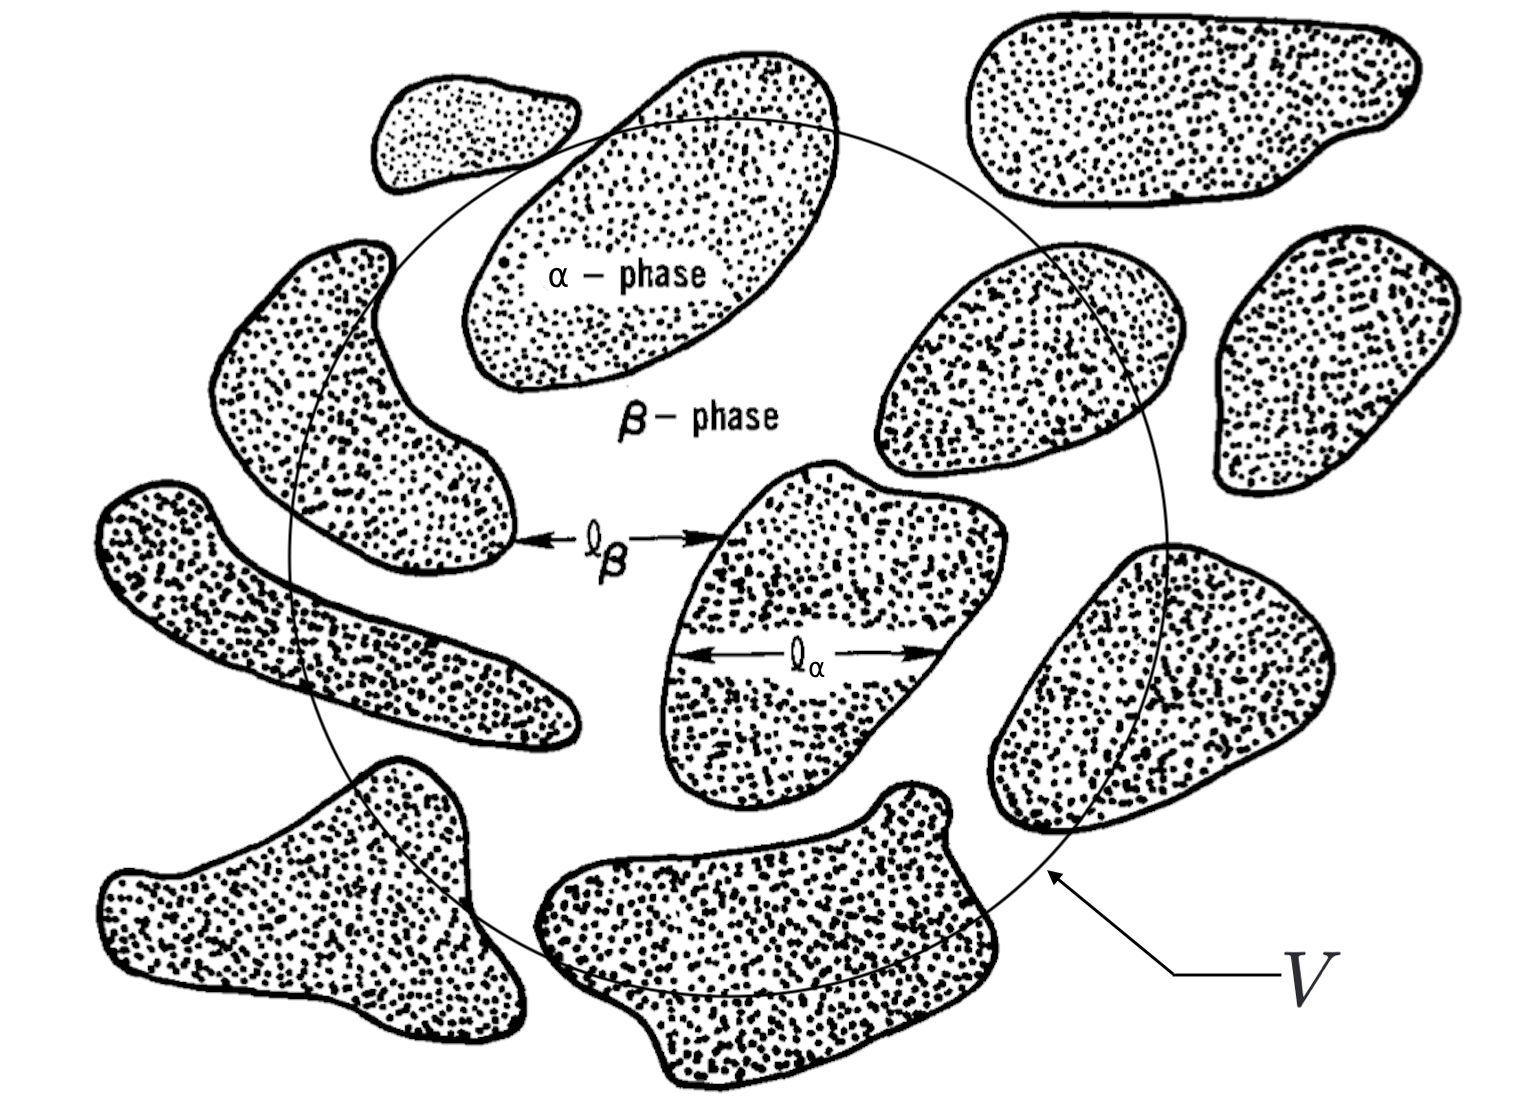
\includegraphics[width=0.6\textwidth]{figures/rev.png}
    \caption[A diagram of the REV]{A diagram of a representative elementary volume (REV), as provided by Whitaker in \cite{whitakerdarcy}}
    \label{fig:rev}
\end{figure}

One advantage of using such a method is that the region over which we solve the continuity and Navier-Stokes equations is smaller, so this is much faster computationally. 
% we can solve the continuity and Navier-Stokes equations for a representative volume macroscopically, instead of solving these equations for each pore in the medium microscopically. Since we do not have to solve for each pore explicitly, it is much faster computationally. 
However, we no longer have information for the velocity $\mathbf{u}$ or pressure $p$ on each pore, and therefore, the real geometry of the porous medium is not modelled exactly.

As shown in Figure \ref{fig:rev}, we consider the porous medium to consist of a single-phase fluid, known as the $\bm{\beta}$\textbf{-phase}, and a solid structure, known as the $\bm{\alpha}$\textbf{-phase}. Associated quantities with each phase will have a subscript $\alpha$ or $\beta$ for the $\alpha$-phase and $\beta$-phase respectively. 

For the fluid, we will also assume that it is incompressible and Newtonian, and that the porous medium is isotropic and homogeneous. 

% \section{Method}
% We will use the following method to write the microscopic conservation equations macroscopically.
% \begin{enumerate}
% 	\item Assume the conservation equations hold true on a \emph{microscopic} level.
% 	\item Use the spatial averaging theorems to express the conservation equations in terms of their phase averages.
% 	% \item Consider the fluctuations from the averages and form a closure model.
% \end{enumerate}

% \section{Implementation}
\section{Definitions}
% Consider a representative elementary volume $V$ in a porous medium consisting of a fluid phase and a solid phase, denoted by $f$ and $s$ respectively. 
Here, we use the definitions given in Section 2 of \cite{whitakerdarcy}. For a quantity $\psi_\beta$ associated with the $\beta$-phase, we define the \textbf{superficial phase average} as
\begin{equation}
\langle\psi_\beta\rangle = \frac{1}{V} \int_{V_\beta} \! \psi_\beta \, \mathrm{d}V, \label{eq:2.1}
\end{equation}
where $V$ is the volume of the REV. We also define the \textbf{intrinsic phase average} as
\begin{equation}
\langle\psi_\beta\rangle^\beta = \frac{1}{V_\beta} \int_{V_\beta} \! \psi_\beta \, \mathrm{d}V, \label{eq:2.2}
\end{equation}
where $V_\beta$ is the volume occupied by the $\beta$-phase in $V$. Note that $\psi_\beta$ can be both a vector and scalar quantity.

We can then define the \textbf{porosity} $\varepsilon_\beta$ as 
\begin{equation}
    \varepsilon_\beta = \frac{V_\beta}{V}, \label{eq:2.3}
\end{equation}
where a \textit{pure fluid} with no solid structure will have $\varepsilon_\beta = 1$ and a \textit{pure solid} will have $\varepsilon_\beta = 0$. From the above equations, we can also see that $\langle\psi_\beta\rangle = \varepsilon_\beta \langle\psi_\beta\rangle^\beta$.

% RELABEL CHAPTER 2 EQUATIONS FROM THIS POINT

\section{Theorems} \label{sec:2.2}
To describe the macroscopic conservation equations from the microscopic conservation equations, we need to use the following theorems \cite{hsu+cheng, whitakerforchheimer}:
\begin{subequations}
\begin{enumerate}
	
	\item Time differentiation
	\begin{equation}
	\left\langle\frac{\partial\psi_\beta}{\partial t}\right\rangle = \frac{1}{V} \int_{V_\beta} \! \frac{\partial}{\partial t}(\psi_\beta) \, \mathrm{d}V = \frac{\partial}{\partial t} \left( \frac{1}{V} \int_{V_\beta} \! \psi_\beta \, \mathrm{d}V \right) = \frac{\partial}{\partial t}\langle\psi_\beta\rangle. \label{eq:2.4a}
	\end{equation}
	
	\item Gradient theorem
	\begin{equation}
	\langle\nabla\psi_\beta\rangle = \nabla\langle\psi_\beta\rangle + \frac{1}{V} \int_{A_{\alpha,\beta}} \! \psi_\beta \hat{\mathbf{n}} \, \mathrm{d}A. \label{eq:2.4b}
	\end{equation}
 
	\item Divergence theorem
	\begin{equation}
	\langle\nabla\cdot\bm{\psi}_\beta\rangle = \nabla\cdot\langle\bm{\psi}_\beta\rangle +\frac{1}{V} \int_{A_{\alpha,\beta}} \! \bm{\psi}_\beta \cdot \hat{\mathbf{n}} \, \mathrm{d}A. \label{eq:2.4c}
	\end{equation}
 
\end{enumerate}
\end{subequations}
Here, $A_{\alpha,\beta}$ is the area of the surface between the $\alpha$-phase and $\beta$-phase, and $\hat{\mathbf{n}}$ is the unit normal vector at the surface between the 2 phases. 

Equations (\ref{eq:2.4b}) and (\ref{eq:2.4c}) are known as the \textbf{spatial averaging theorems} and a proof of these theorems is provided by Whitaker in \cite{spatialavethm} but will be omitted from this report.

We assume that the porous medium is rigid and stationary, and require the no-slip boundary condition to be satisfied:
\begin{equation}
	\mathbf{u}_{\beta} =\mathbf{0} \quad \text{on} \quad A_{\alpha,\beta}. \label{eq:2.5} % \quad adds a space
\end{equation}
Therefore, when $\bm{\psi}_\beta = \mathbf{u}_{\beta}$, the boundary terms in the above theorems vanish.

\section{Continuity Equation}
With these definitions and theorems, we are now ready to give a macroscopic description of the fluid equations. We begin with the microscopic continuity equation, given by

\begin{equation}
    \frac{\partial\rho_{\beta}}{\partial t} + \nabla \cdot (\rho_{\beta} \mathbf{u}_{\beta}) = 0, \label{eq:2.6}
\end{equation}
where $\rho_\beta$ is the density of the fluid. As we assume the fluid is incompressible, we can therefore ignore the variations of $\rho$ in the REV. Thus, $\rho = \rho_{\beta}$ and $\frac{\partial\rho}{\partial t} = 0$. 
% Here, we assume the fluid properties are unchanged in the REV, i.e. $\rho = \rho_{\beta}$ and $\mu = \mu_{\beta}$, and we omit the subscript $\beta$ from these variables.
% We have assumed the fluid is incompressible and we can therefore ignore the variations of $\rho$ in the REV. Thus, $\rho = \rho_{\beta}$ and $\frac{\partial\rho}{\partial t} = 0$. 

Taking the phase average, we get
% \begin{equation*}
%     \left\langle\frac{\partial\rho}{\partial t}\right\rangle + \langle\nabla\cdot(\rho\mathbf{u}_{\beta})\rangle = 0.
% \end{equation*}

% Clearly, the first term vanishes as $\rho$ is unchanged in the REV, so we are left with 
\begin{equation*}
	\langle\nabla\cdot(\rho\mathbf{u}_{\beta})\rangle = 0. 
\end{equation*}

Using the volume averaging divergence theorem (\ref{eq:2.4c}) and the boundary condition (\ref{eq:2.5}), we obtain the equation:
\begin{equation*}
	\rho\nabla\cdot\langle\mathbf{u}_{\beta}\rangle + \cancel{\frac{1}{V} \int_{A_{\alpha,\beta}} \! \rho\mathbf{u}_{\beta} \cdot \hat{\mathbf{n}} \, \mathrm{d}A} = 0.
\end{equation*}

As the fluid has non-zero density, we therefore obtain the following equation \textbf{macroscopic continuity equation}:
\begin{equation}
    \boxed{\nabla\cdot\langle\mathbf{u}_{\beta}\rangle = 0.} \label{eq:2.7}
\end{equation}

This can also be rewritten in terms of the intrinsic phase average as
\begin{equation}
	\nabla\cdot(\varepsilon_\beta\langle\mathbf{u}_{\beta}\rangle^\beta) = 0. \label{eq:2.8}
\end{equation}

\section{Navier-Stokes Equations}
To describe the motion of a viscous fluid, we use equation (6.39) from \cite[Chapter~6]{fmnotes}:
% The Navier-Stokes equations that also govern the (microscopic) fluid flow can be written as
\begin{equation}
	\rho_{\beta}\left(\frac{\partial \mathbf{u}_{\beta}}{\partial t} + \mathbf{u}_{\beta} \cdot \nabla \mathbf{u}_{\beta} \right) = -\nabla p_{\beta} + \mu_{\beta} \nabla^2 \mathbf{u}_{\beta} + \rho_{\beta} \mathbf{g}, \label{eq:2.9}
\end{equation}
where $p_\beta$ and $\mu_\beta$ are the pressure and viscosity of the $\beta$-phase and $\mathbf{g}$ is an external body force different from the porous ones, such as the force due to gravitational acceleration. %For simplicity, we will neglect this ter
m.

As before, we will ignore the variations in $\rho_{\beta}$ due to the incompressibility condition. We will also ignore the variations in $\mu_{\beta}$ within the averaging volume. %assume the density $\rho_{\beta}$ and kinematic viscosity $\mu_{\beta}$ are unchanged in the REV and omit the subscript $\beta$ from these variables.

Taking the phase average of the equation (\ref{eq:2.9}), we get
\begin{equation}
	\rho\left\langle\frac{\partial\mathbf{u}_{\beta}}{\partial t}\right\rangle + \rho\langle\nabla\cdot(\mathbf{u}_{\beta}\mathbf{u}_{\beta})\rangle = -\langle\nabla p_{\beta}\rangle + \mu\langle\nabla\cdot\nabla\mathbf{u}_{\beta}\rangle +  \rho\langle\mathbf{g}\rangle, \label{eq:2.10} % \rho\langle\mathbf{g}\rangle
\end{equation}
where we have also rewritten $\nabla^2\mathbf{u}_{\beta}=\nabla\cdot\nabla\mathbf{u}_{\beta}$, and $\mathbf{u}_{\beta} \cdot \nabla \mathbf{u}_{\beta}=\nabla \cdot (\mathbf{u}_{\beta}\mathbf{u}_{\beta})$. The latter equality can be shown using Einstein summation convention and the incompressibility assumption:
\begin{equation}
    \nabla \cdot (\mathbf{u}\mathbf{u}) = \frac{\partial}{\partial x_j}(u_iu_j) = u_i\frac{\partial}{\partial x_j}(u_j) + u_j\frac{\partial}{\partial x_j}(u_i) = \cancel{\mathbf{u}(\nabla \cdot \mathbf{u})} + \mathbf{u} \cdot \nabla \mathbf{u}. \label{eq:2.11}
\end{equation}

As $\mathbf{g}$ is an external body force, we can assume that it does not vary within the averaging volume and we therefore have $\langle\mathbf{g}\rangle = \mathbf{g}\langle 1\rangle$, where $\langle 1\rangle = \frac{V_\beta}{V} = \varepsilon_\beta$ using definition (\ref{eq:2.1}).

Using the spatial averaging theorems in Section \ref{sec:2.2} and the no-slip boundary condition (\ref{eq:2.5}), (\ref{eq:2.10}) becomes
\begin{align*}
	&\rho\frac{\partial}{\partial t}\langle\mathbf{u}_{\beta}\rangle + \rho\nabla\cdot\langle\mathbf{u}_{\beta}\mathbf{u}_{\beta}\rangle + \cancel{\frac{1}{V} \int_{A_{\alpha,\beta}} \! \rho\mathbf{u}_{\beta}\mathbf{u}_{\beta} \hat{\mathbf{n}} \, \mathrm{d}A} \\ &= -\nabla\langle p_{\beta}\rangle - \frac{1}{V}\int_{A_{\alpha,\beta}} \! p_{\beta} \hat{\mathbf{n}} \, \mathrm{d}A + \mu\nabla\cdot\langle\nabla\mathbf{u}_{\beta}\rangle + \frac{1}{V}\int_{A_{\alpha,\beta}} \! \mu\nabla\mathbf{u}_{\beta}\cdot \hat{\mathbf{n}} \, \mathrm{d}A + \rho\varepsilon_\beta\mathbf{g}\\ &= -\nabla\langle p_{\beta}\rangle + \mu\nabla^2\langle\mathbf{u}_{\beta}\rangle + \cancel{\frac{\mu}{V}\nabla\cdot \int_{A_{\alpha,\beta}} \! \mathbf{u}_{\beta} \cdot \hat{\mathbf{n}} \, \mathrm{d}A} + \frac{1}{V}\int_{A_{\alpha,\beta}} \! (-p_{\beta}\mathbf{I} + \mu\nabla\mathbf{u}_{\beta})\cdot \hat{\mathbf{n}} \, \mathrm{d}A + \rho\varepsilon_\beta\mathbf{g},
\end{align*}
where $\mathbf{I}$ is the identity matrix. Writing this out gives
\begin{equation}
    \boxed{\rho\frac{\partial}{\partial t}\langle\mathbf{u}_{\beta}\rangle + \rho\nabla\cdot\langle\mathbf{u}_{\beta}\mathbf{u}_{\beta}\rangle = -\nabla\langle p_{\beta}\rangle + \mu\nabla^2\langle\mathbf{u}_{\beta}\rangle + \rho\varepsilon_\beta\mathbf{g} + \mathbf{B},} \label{eq:2.12}
\end{equation}
where we define
% Applying the volume-averaged gradient theorem again on the third term of the RHS gives
% \begin{equation}
% 	\rho\frac{\partial}{\partial t}\langle\mathbf{u}_{\beta}\rangle  + \rho\nabla\cdot\langle\mathbf{u}_{\beta}\mathbf{u}_{\beta}\rangle = -\nabla\langle p_{\beta}\rangle + \mu\nabla^2\langle\mathbf{u}_{\beta}\rangle + \cancel{\frac{\mu}{V}\nabla\cdot \int_{A_{\alpha,\beta}} \! \mathbf{u}_{\beta} \cdot \hat{\mathbf{n}} \, \mathrm{d}A} + \mathbf{B}, \label{eq:2.10}
% \end{equation}
% where $\mathbf{I}$ is the identity matrix and
\begin{equation}
	\mathbf{B} = \frac{1}{V}\int_{A_{\alpha,\beta}} \! (-p_{\beta}\mathbf{I} + \mu\nabla\mathbf{u}_{\beta})\cdot \hat{\mathbf{n}} \, \mathrm{d}A \label{eq:2.13}
\end{equation}
as the total drag force per unit volume due to the presence of solid particles, consisting of a pressure term and a viscous term.

Notice that in (\ref{eq:2.12}), we have the average of a product ($\langle\mathbf{u}_\beta\mathbf{u}_\beta\rangle$ which we want to eliminate. To eliminate the average of a product $\langle\psi_{\beta}\xi_{\beta}\rangle$, we make use of the velocity decomposition as given by Gray \cite{gray}:
\begin{subequations}
\begin{align}
	\psi_\beta &= \langle\psi_\beta\rangle^\beta + \psi_\beta', \label{eq:2.14a} \\
	\xi_\beta &= \langle\xi_\beta\rangle^\beta + \xi_\beta', \label{eq:2.14b}
\end{align}
where we decompose each quantity into the sum of the intrinsic $\beta$-phase average and a fluctuating component. We also assume the associated $\alpha$-phase quantities are zero:
\begin{equation}
	\psi_\alpha = \psi_\alpha' = 0 \quad \text{and} \quad \xi_\alpha = \xi_\alpha' = 0. \label{eq:2.14c}
\end{equation}
Assuming the averages of $\psi_\beta$ and $\xi_\beta$ are well-behaved, we have that the averages of the fluctuations vanish:
\begin{equation}
	\langle\psi_\beta'\rangle = \langle\psi_\beta'\rangle^\beta = 0 \quad \text{and} \quad \langle\xi_\beta'\rangle = \langle\xi_\beta'\rangle^\beta = 0,\label{eq:2.14d}
\end{equation}
and the variation of an average quantity is the average quantity itself:
\begin{equation}
	\langle\langle\psi_\beta\rangle^\beta\rangle = \langle\langle\psi_\beta\rangle^\beta\rangle^\beta = \langle\psi_\beta\rangle^\beta \quad \text{and} \quad \langle\langle\psi_\beta\rangle\rangle = \langle\langle\psi_\beta\rangle\rangle^\beta = \langle\psi_\beta\rangle.\label{eq:2.14e}
 \end{equation}
\end{subequations} \label{eq:2.14}
Then
\begin{align}
	\langle\psi_\beta\xi_\beta\rangle &= \varepsilon_\beta\langle\psi_\beta\xi_\beta\rangle^\beta \nonumber \\
	&= \varepsilon_\beta \left[\langle\langle\psi_\beta\rangle^\beta\langle\xi_\beta\rangle^\beta\rangle^\beta + \langle\psi_\beta'\langle\xi_\beta\rangle^\beta\rangle^\beta + \langle\langle\psi_\beta\rangle^\beta\xi_\beta'\rangle^\beta+\langle\psi_\beta'\xi_\beta'\rangle^\beta\right]. \label{eq:2.15}
\end{align}
Assuming $\langle\psi_\beta\rangle^\beta$ and $\langle\xi_\beta\rangle^\beta$ are constant in REV and using (\ref{eq:2.14d}), we get
\begin{align*}
	&\langle\langle\psi_\beta\rangle^\beta\langle\xi_\beta\rangle^\beta\rangle^\beta = \langle\psi_\beta\rangle^\beta\cdot\langle\xi_\beta\rangle^\beta, \\
    &\langle\psi_\beta'\langle\xi_\beta\rangle^\beta\rangle^\beta = \langle\psi_\beta'\rangle^\beta\cdot\langle\xi_\beta\rangle^\beta = 0, \\
    &\langle\langle\psi_\beta\rangle^\beta\xi_\beta'\rangle^\beta = \langle\psi_\beta\rangle^\beta\cdot\langle\xi_\beta'\rangle^\beta = 0.
\end{align*}
Finally, assuming $\psi_\beta' \ll \langle\psi_\beta\rangle^\beta$ and $\xi_\beta' \ll \langle\xi_\beta\rangle^\beta$, $\langle\psi_\beta'\xi_\beta'\rangle^\beta$ must be negligible and can therefore be taken as 0, giving
\begin{equation}
	\boxed{\langle\psi_\beta\xi_\beta\rangle = \varepsilon_\beta\langle\psi_\beta\rangle^\beta\langle\xi_\beta\rangle^\beta.} \label{eq:2.16}
\end{equation}

Using (\ref{eq:2.16}) in (\ref{eq:2.12}), we get
\begin{equation}
    \rho\frac{\partial}{\partial t}\langle\mathbf{u}_{\beta}\rangle + \rho\nabla\cdot(\varepsilon_\beta\langle\mathbf{u}_{\beta}\rangle^\beta\langle\mathbf{u}_{\beta}\rangle^\beta) = -\nabla\langle p_{\beta}\rangle + \mu\nabla^2\langle\mathbf{u}_{\beta}\rangle + \rho\varepsilon_\beta\mathbf{g} + \mathbf{B}. \label{eq:2.17}
\end{equation}
Rewriting the second term in terms of the superficial phase average and dividing by $\rho$, we get
% Returning to the superficial phase average and dividing by $\rho$, we get
\begin{equation}
    \boxed{\frac{\partial}{\partial t}\langle\mathbf{u}_{\beta}\rangle + \nabla\cdot\left(\frac{\langle\mathbf{u}_{\beta}\rangle\langle\mathbf{u}_{\beta}\rangle}{\varepsilon_\beta}\right) = -\frac{1}{\rho}\nabla\langle p_{\beta}\rangle + \nu\nabla^2\langle\mathbf{u}_{\beta}\rangle + \varepsilon_\beta\mathbf{g} + \frac{1}{\rho}\mathbf{B},} \label{eq:2.18}
\end{equation}
where $\nu = \frac{\mu}{\rho}$ is the \textbf{kinematic viscosity}.


\section{Closure Modelling for the Drag Force due to the Porous Medium} \label{sec:2.5}
% \todo[inline, color=green!40]{discuss closure, see \cite{hsu+cheng}, mention the darcy/forchheimer terms}
% \textcolor{blue}{ See \cite{whitakerforchheimer, whitakerdarcy, hsu+cheng} }

To obtain closure for the body force term $\mathbf{B}$ given by (\ref{eq:2.13}), we use the model presented by Hsu \& Cheng in \cite{hsu+cheng}, where we consider the porous medium to be a dilute random array of spheres of diameter $d_p$ that do not interact within the medium. It can then be shown that $\mathbf{B}$ reduces to Ergun's expression \cite{ergun}:

\begin{equation}
    \mathbf{B} = -\left[\frac{\mu\varepsilon_\beta}{K}\langle\mathbf{u}_\beta\rangle + \rho\frac{F_\varepsilon\varepsilon_\beta}{\sqrt{K}}\langle\mathbf{u}_\beta\rangle\left|\langle\mathbf{u}_\beta\rangle\right|\right], \label{eq:2.19}
\end{equation}
where the \textbf{permeability} $K$ is related to the porosity by
\begin{equation}
    K = \frac{\varepsilon_\beta^3 d_p^2}{150(1-\varepsilon_\beta)^2}, \label{eq:2.20}
\end{equation}
and is a property of a material that describes how easily a fluid can flow through it. $F_\varepsilon$ is the \textbf{Forchheimer coefficient}, a geometric function of the porous medium given by
\begin{equation}
    F_\varepsilon = \frac{1.75}{\sqrt{150\varepsilon_\beta^3}}. \label{eq:2.21}
\end{equation}
The equation (\ref{eq:2.19}) consists of a linear term and a non-linear term, which correspond to the viscous (Darcy) drag term and the inertial (Forchheimer) drag term respectively. 


Therefore the \textbf{macroscopic momentum equation} for an incompressible flow in a constant porosity medium is
\begin{subequations} \label{eq:2.22}
\begin{equation}
    \boxed{\frac{\partial}{\partial t}\langle\mathbf{u}_{\beta}\rangle + \nabla\cdot\left(\frac{\langle\mathbf{u}_{\beta}\rangle\langle\mathbf{u}_{\beta}\rangle}{\varepsilon_\beta}\right) = -\frac{1}{\rho}\nabla\langle p_{\beta}\rangle + \nu\nabla^2\langle\mathbf{u}_{\beta}\rangle + \mathbf{F}} \label{eq:2.22a}
\end{equation}
with
\begin{equation}
    \boxed{\mathbf{F} = \varepsilon_\beta\mathbf{g} - \left[\frac{\nu\varepsilon_\beta}{K}\langle\mathbf{u}_\beta\rangle + \frac{F_\varepsilon\varepsilon_\beta}{\sqrt{K}}\langle\mathbf{u}_\beta\rangle\left|\langle\mathbf{u}_\beta\rangle\right|\right].} \label{eq:2.22b}
\end{equation}
\end{subequations}
In terms of the intrinsic phase average, the above equations are
\begin{subequations}
\begin{equation}
    \frac{\partial}{\partial t}\langle\mathbf{u}_\beta\rangle^\beta + \nabla\cdot\left(\langle\mathbf{u}_\beta\rangle^\beta\langle\mathbf{u}_\beta\rangle^\beta\right) = -\frac{1}{\rho}\nabla\langle p_\beta\rangle^\beta + \nu\nabla^2\langle\mathbf{u}_\beta\rangle^\beta + \mathbf{\tilde{F}} \label{eq:2.23a}
\end{equation}
with
\begin{equation}
    \mathbf{\tilde{F}} = \mathbf{g} - \left[\frac{\nu\varepsilon_\beta}{K}\langle\mathbf{u}_\beta\rangle^\beta + \frac{F_\varepsilon\varepsilon_\beta^2}{\sqrt{K}}\langle\mathbf{u}_\beta\rangle^\beta|\langle\mathbf{u}_\beta\rangle^\beta|\right]. \label{eq:2.23b}
\end{equation}
\end{subequations} \label{eq:2.23}

% \section{Dimensionless numbers}

%--------------------------------------------------------------------------------------
%	LATTICE BOLTZMANN METHOD
%--------------------------------------------------------------------------------------

\chapter{The Lattice Boltzmann Method} \label{chap:3}
% \todo[inline, color=blue!20]{insert motivation behind lbm, some history}
% \todo[inline, color=blue!20]{advantages and limitations}
% \textcolor{blue}{ Lattice Boltzmann Textbook for sections 3.1, 3.2 }
% \todo[inline, color=blue!20]{rewrite ch introduction}
The lattice Boltzmann method (LBM) is a computational fluid dynamics method developed from lattice gas models \cite[Chapter~2]{lbtextbook}. It is based on \emph{mesoscopic} kinetic theory, describing the behaviour of a collection of particles, instead of the motion of individual particles, as described by Viggen in \cite[Chapter~1]{lbfund} and Kr{\"u}ger et al. in \cite[Section~1.3]{lbtextbook}. %Time, space and velocity are discretised to give the discretised Boltzmann equation. 

% making LBM easier to implement, as described in \cite{lbch3}. LBM is also well-suited to simulate complex geometries, such as those in porous media, making it our method of choice in this project. Conventional numerical methods, such as the finite difference (FD) method, often have to discretise the non-linear advection term $\mathbf{u}\cdot\nabla\mathbf{u}$ and consider the non-linear interaction between lattice nodes, increasing the complexity of the computations. Comparatively, interactions between nodes in LBM are linear, as the detail lies within the nodes themselves, with the heaviest computations being local. 

% The Boltzmann equation, which LBM is based off of, is discretised, making use


% Specifically, it is a discretisation of the Boltzmann equation, making use of the fact that time, space and velocity are discretised. Fundamentally, the lattice Boltzmann method involves sending and receiving information to and from the neighbouring lattice nodes in the direction of the discrete velocities.

% from a lattice node is sent to the neighbouring nodes in the direction of the discrete velocities as part of a process known as \emph{streaming}.

% This chapter discusses the force-free lattice Boltzmann method applied first to a pure fluid, and then to a flow through porous media. Various boundary condition schemes are discussed, as well as their implementation, before considering the forces from the porous medium. 

% This chapter develops and applies the method first to a pure fluid, and then to fluid flow through porous media. Various boundary condition schemes are discussed, be %see how the LBM is used to model blood flow through an aneurysm.

% LBM was developed from lattice gas models \cite[Chapter~2]{lbtextbook}, and is based on \emph{mesoscopic} kinetic theory, describing the behaviour of a collection of particles, instead of the motion of individual particles \cite[Chapter~1]{lbtextbook}. 

% \todo[inline, color=blue!20]{need basic desc of lbm?}

As described in \cite[Chapter~3]{lbtextbook}, the LBM is well-suited to simulating complex geometries, such as those in porous media, and is simpler to implement compared to other numerical methods as it is based on the Boltzmann equation. Conventional numerical methods, such as the finite difference method (detailed in Section 2.1.1 of \cite{lbtextbook}), often have to discretise the non-linear advection term $\mathbf{u}\cdot\nabla\mathbf{u}$ (as seen in equation (\ref{eq:2.9})) and consider the non-linear interaction between lattice nodes, increasing the complexity of the computations. Comparatively, interactions between nodes in LBM are linear with the heaviest computations being local, as the detail lies within the nodes themselves. 

In this chapter, we will first give a basic introduction to kinetic theory in Section \ref{sec:3.1}, before outlining the LBM in Section \ref{sec:3.2} for pure fluids and fluid flows through porous media without forces. Section \ref{sec:3.3} explains how several boundary conditions work and how they can be implemented and finally, Section \ref{sec:3.4} discusses how we can implement the forces discussed in Section \ref{sec:2.5}.

\section{Kinetic Theory} \label{sec:3.1}
\textbf{Mesoscopic kinetic theory} is a theory between macroscopic and microscopic viewpoints that describes the distribution of particles in a fluid. It is typically applied to dilute monatomic gases, where molecules spend very little time colliding and almost always collide 1-on-1. This does not hold true for dense gases or liquids, but it is possible to formulate a kinetic theory for these fluids, which we will not discuss. More details about this can be seen in \cite{liquidkin}. We will also assume that the behaviour of polyatomic and monatomic gases is the same.

A \textbf{particle distribution function} $f(\mathbf{x},\bm{\xi},t)$ is used to describe the probability of a group of particles being at position $\mathbf{x}$ with velocity $\bm{\xi}$ at time $t$. We consider $f$ to be a generalisation of the density $\rho$ that takes the microscopic particle velocity $\bm{\xi}$ into account.
\newpage
From its \textbf{moments}, which are integrals of $f$ weighted with some function of $\bm{\xi}$ over the entire velocity space, we can connect the distribution function $f$ to the macroscopic \textbf{mass density} $\rho$ and the macroscopic \textbf{momentum density} $\rho\mathbf{u}$ through the following equations:
\begin{subequations}
\begin{align}
	\rho(\mathbf{x},t) &= \int \! f(\mathbf{x},\bm{\xi},t) \, \mathrm{d}^n\xi, \label{eq:3.1a} \\
	\rho(\mathbf{x},t)\mathbf{u}(\mathbf{x},t) &= \int \! \bm{\xi}f(\mathbf{x},\bm{\xi},t) \, \mathrm{d}^n\xi, \label{eq:3.1b}
\end{align}
where $n$ is the number of dimensions.
\end{subequations} \label{eq:3.1}

To describe how $f$ evolves in time, we consider its total time derivative
\begin{equation}
    \frac{\mathrm{d}f}{\mathrm{d}t} = \left( \frac{\partial f}{\partial t} \right) \frac{\mathrm{d}t}{\mathrm{d}t} + \left( \frac{\partial f}{\partial x_\mu}\right) \frac{\mathrm{d}x_\mu}{\mathrm{d}t} + \left( \frac{\partial f}{\partial \xi_\mu} \right) \frac{\mathrm{d} \xi_\mu}{\mathrm{d} t}, \label{eq:3.2}
\end{equation}
where we use Einstein summation convention to indicate that $f$ is differentiated over each term in $\mathbf{x}$ and $\bm{\xi}$, with $\mu=1,\dots,\text{ }n$. To simplify this further, we use the fact that $\frac{\mathrm{d}t}{\mathrm{d}t} = 1$ and we define the particle velocity as $\xi_\mu=\frac{\mathrm{d}x_\mu}{\mathrm{d}t}$. Further, using Newton's second law $\mathbf{F} = \rho\frac{\mathrm{d} \bm{\xi}}{\mathrm{d} t}$, we notice that $\frac{\mathrm{d} \xi_\mu}{\mathrm{d} t}$ can be rewritten as $\frac{F_\mu}{\rho}$, where $\mathbf{F}$ is the specific body force. This gives
\begin{equation}
    \frac{\mathrm{d}f}{\mathrm{d}t} = \frac{\partial f}{\partial t} + \xi_\mu\frac{\partial f}{\partial x_\mu} + \frac{F_\mu}{\rho} \frac{\partial f}{\partial \xi_\mu}. \label{eq:3.3}
\end{equation}

% When a fluid has been left alone for a sufficient amount of time, we assume that it reaches a state of equilibrium, denoted by an \textbf{equilibrium function} $f^{\mathrm{eq}}(\mathbf{x},\bm{\xi},t)$, which has the same moments of density as $f$. It is also known as the \textbf{Maxwell-Boltzmann distribution}, which is given by
% \begin{equation}
%     f^{\mathrm{eq}}(\mathbf{x}, |\mathbf{v}|,t) = \rho\left(\frac{\rho}{2\pi p}\right)^{d/2}e^{-p|\bm{\xi}-\mathbf{u}|^2/(2\rho)}, \label{eq:3.4}
% \end{equation}
% for some mean velocity $\mathbf{u}$.

A common notation to use is $\Omega(f) = \frac{\mathrm{d}f}{\mathrm{d}t}$ for the total derivative, which is a source term known as the \textbf{collision operator}. It represents the local redistribution of $f$ due to collisions. Overall, we can rewrite (\ref{eq:3.2}) as
\begin{equation}
     \frac{\partial f}{\partial t} + \xi_\mu\frac{\partial f}{\partial x_\mu} + \frac{F_\mu}{\rho} \frac{\partial f}{\partial \xi_\mu} = \Omega(f). \label{eq:3.4}
\end{equation}
Equation (\ref{eq:3.3}) is also known as the \textbf{Boltzmann equation}, with the first two terms on the RHS representing the advection of the distribution function $f$ with velocity $\bm{\xi}$, and the third term representing the forces affecting the velocity $\bm{\xi}$. 

As we know, collisions conserve mass, momentum and also energy, which means that the 0th, 1st and 2nd moments of the collision operator are equal to 0, as given in equations (1.48a) - (1.48c) in \cite{lbtextbook}:
\begin{subequations} \label{eq:3.5}
\begin{align}
    \int \! \Omega(f) \, \mathrm{d}^n\xi = 0, \label{eq:3.5a} \\
    \int \! \bm{\xi} \Omega(f) \, \mathrm{d}^n\xi = 0, \label{eq:3.5b} \\
    \int \! |\bm{\xi}|^2 \Omega(f) \, \mathrm{d}^n\xi = 0. \label{eq:3.5c}
\end{align}
\end{subequations}
According to Kr{\"u}ger et al. in \cite[Section 1.3.4]{lbtextbook}, Boltzmann's original form of $\Omega(f)$ is complicated, making it difficult to implement in LBM. Instead, the simplest collision operator used in LBM that satisfies (\ref{eq:3.5}), i.e. conserves mass, momentum and energy, is the \textbf{BGK (Bhatnagar-Gross-Krook) collision operator}, given by:
\begin{equation}
    \Omega(f) = -\frac{1}{\tau}(f - f^{\mathrm{eq}}), \label{eq:3.6}
\end{equation}
where $\tau$ is the \textbf{relaxation time}, or the time taken for $f$ to approach $f^{\mathrm{eq}}$. The \textbf{equilibrium distribution function}, denoted by $f^{\mathrm{eq}}$ describes the state of equilibrium that the fluid reaches when it has been left alone for a sufficient amount of time. It is also known as the \textbf{Maxwell-Boltzmann distribution}, which is given by equation (1.45) in \cite{lbtextbook}:
\begin{equation}
    f^{\mathrm{eq}}(\mathbf{x}, |\bm{\xi}-\mathbf{u}|,t) = \rho\left(\frac{\rho}{2\pi p}\right)^{n/2}e^{-p|\bm{\xi}-\mathbf{u}|^2/(2\rho)}, \label{eq:3.7}
\end{equation}
for some mean velocity $\mathbf{u}$.

Another popular choice of collision operator is the multiple-relaxation-time (MRT) operator, which is known to be more accurate and stable than the BGK operator \cite{mrt}, but is also more difficult to implement, requiring more resources if not coded efficiently \cite[Section 10.7.3]{lbtextbook}. As we are using the BGK operator in this project, the MRT operator will not be discussed further, but \cite{mrt} will provide more information on this operator.

\section{The Force-Free Lattice Boltzmann Equations} \label{sec:3.2}
% \todo[inline, color=blue!20]{reorder this section to make it read easier}
We first consider the force-free lattice Boltzmann equations, taking $\mathbf{F} = \mathbf{0}$. The Boltzmann BGK equation ((\ref{eq:3.4}) with (\ref{eq:3.6})) therefore becomes
\begin{equation}
    \frac{\partial f}{\partial t} + \xi_\beta\frac{\partial f}{\partial x_\beta} = -\frac{1}{\tau}(f - f^{\mathrm{eq}}). \label{eq:3.8}
\end{equation}
In order to solve this numerically, we need to discretise time $t$, space $\mathbf{x}$, as well as the velocity space $\bm{\xi}$, which we refer to as $\mathbf{c}_k$ in the discrete space \cite[Sections 3.4-3.5]{lbtextbook}. 

Our main object of interest is the \textbf{discrete-velocity distribution function} $f_k(\mathbf{x},t)$, which describes the probability of a group of particles being at position $\mathbf{x}$ with velocity $\mathbf{c}_k$ at time $t$. We take the discrete versions of (\ref{eq:3.1}) to find the moments of $f_k$, obtaining the following equations:
\begin{subequations} \label{eq:3.9}
\begin{align}
    \rho(\mathbf{x},t) &= \sum_k f_k(\mathbf{x},t), \label{eq:3.9a} \\
    \rho\mathbf{u}(\mathbf{x},t) &= \sum_k \mathbf{c}_k f_k(\mathbf{x},t). \label{eq:3.9b}
\end{align}
\end{subequations}
Here, $\mathbf{x}$ refers to a discrete set of points in a square lattice in space with lattice spacing $\Delta x$, and $\mathbf{c}_k$ is a discrete velocity. Since time is also discrete, $f_k$ is only defined at certain times $t$ with time-step $\Delta t$. For numerical simulations, we will use \textbf{lattice units}, which are an artificial set of units scaled by $\Delta x = 1$ and $\Delta t = 1$. This allows us to use the \textbf{law of similarity} \cite[Section~1.2]{lbtextbook}, which states that fluid flows that share the same dimensionless numbers exhibit the same physics, to compare systems without having to convert units. 

% \begin{figure}[!hbt]
% \centering
% \begin{tikzpicture}[thick,scale=1, every node/.style={scale=1}, >={Latex[length=3mm, width=2mm]}]
    \draw[gray, dashed, thin] (0, 0) rectangle (4,4);
    \node at (-0.3, -0.3) {$\mathbf{c}_7$};
    \node at (-0.35, 2) {$\mathbf{c}_2$};
    \node at (-0.3, 4.3) {$\mathbf{c}_6$};
    \node at (2, -0.3) {$\mathbf{c}_4$};
    \node at (2.6, 2.2) {$\mathbf{c}_0$};
    \node at (2, 4.3) {$\mathbf{c}_3$};
    \node at (4.3, -0.3) {$\mathbf{c}_8$};
    \node at (4.35, 2) {$\mathbf{c}_1$};
    \node at (4.3, 4.3) {$\mathbf{c}_5$};
    \foreach \n in {0, 1, 2}
    \foreach \m in {0, 1, 2}{
    \filldraw[black] (2*\n, 2*\m) circle (2pt);
    }
    \draw[black, ->, thin] (2, 2) -- (0, 0);
    \draw[black, ->, thin] (2, 2) -- (0, 2);
    \draw[black, ->, thin] (2, 2) -- (0, 4);
    \draw[black, ->, thin] (2, 2) -- (2, 0);
    \draw[black, ->, thin] (2, 2) -- (2, 4);
    \draw[black, ->, thin] (2, 2) -- (4, 0);
    \draw[black, ->, thin] (2, 2) -- (4, 2);
    \draw[black, ->, thin] (2, 2) -- (4, 4);
\end{tikzpicture}
% \caption{The D2Q9 lattice arrangement.} \label{fig:d2q9}
% \end{figure}

The discrete velocities $\textbf{c}_k$, together with the weighting coefficients $w_k$, form \textbf{velocity sets}. These are usually denoted D$n$Q$m$, where $n$ is the number of spatial directions and $m$ is the number of velocities. In this project, we use the D2Q9 configuration shown in Figure \ref{fig:d2q9}, with the explicit velocities and weighting coefficients given in Table \ref{table:d2q9}.

% \begin{table} [!htb]
% \centering
%     \begin{tabular}{c||c|c|c|c|c|c|c|c|c}
%     \hline
%     $k$ & 0 & 1 & 2 & 3 & 4 & 5 & 6 & 7 & 8  \\
%     \hline
%     & & & & & & & & &\\ [-2ex]
%     $w_k$ & $\frac{4}{9}$ & $\frac{1}{9}$ & $\frac{1}{9}$ & $\frac{1}{9}$ & $\frac{1}{9}$ & $\frac{1}{36}$ & $\frac{1}{36}$ & $\frac{1}{36}$ & $\frac{1}{36}$ \\ [1ex]
%     \hline
%     $c_{kx}$ & 0 & +1 & -1 & 0 & 0 & +1 & -1 & -1 & +1 \\
%     \hline
%     $c_{ky}$ & 0 & 0 & 0 & +1 & -1 & +1 & +1 & -1 & -1 \\
%     \hline
%     $k'$ & 0 & 2 & 1 & 4 & 3 & 7 & 8 & 5 & 6 \\
%     \hline
%     \end{tabular}
%     \caption{D2Q9 lattice arrangement with the velocities and weighting coefficients shown explicitly. $k'$ indicates the direction opposite $k$.}
%     \label{table:d2q9}
% \end{table}

\begin{figure}[!hbt]
\centering
\begin{tikzpicture}[thick,scale=1, every node/.style={scale=1}, >={Latex[length=3mm, width=2mm]}]
    \draw[gray, dashed, thin] (0, 0) rectangle (4,4);
    \node at (-0.3, -0.3) {$\mathbf{c}_7$};
    \node at (-0.35, 2) {$\mathbf{c}_2$};
    \node at (-0.3, 4.3) {$\mathbf{c}_6$};
    \node at (2, -0.3) {$\mathbf{c}_4$};
    \node at (2.6, 2.2) {$\mathbf{c}_0$};
    \node at (2, 4.3) {$\mathbf{c}_3$};
    \node at (4.3, -0.3) {$\mathbf{c}_8$};
    \node at (4.35, 2) {$\mathbf{c}_1$};
    \node at (4.3, 4.3) {$\mathbf{c}_5$};
    \foreach \n in {0, 1, 2}
    \foreach \m in {0, 1, 2}{
    \filldraw[black] (2*\n, 2*\m) circle (2pt);
    }
    \draw[black, ->, thin] (2, 2) -- (0, 0);
    \draw[black, ->, thin] (2, 2) -- (0, 2);
    \draw[black, ->, thin] (2, 2) -- (0, 4);
    \draw[black, ->, thin] (2, 2) -- (2, 0);
    \draw[black, ->, thin] (2, 2) -- (2, 4);
    \draw[black, ->, thin] (2, 2) -- (4, 0);
    \draw[black, ->, thin] (2, 2) -- (4, 2);
    \draw[black, ->, thin] (2, 2) -- (4, 4);
\end{tikzpicture}
\caption{The D2Q9 lattice arrangement.} \label{fig:d2q9}
\end{figure}

\begin{table} [!htb]
\centering
    \begin{tabular}{c||c|c|c|c|c|c|c|c|c}
    \hline
    $k$ & 0 & 1 & 2 & 3 & 4 & 5 & 6 & 7 & 8  \\
    \hline
    & & & & & & & & &\\ [-2ex]
    $w_k$ & $\frac{4}{9}$ & $\frac{1}{9}$ & $\frac{1}{9}$ & $\frac{1}{9}$ & $\frac{1}{9}$ & $\frac{1}{36}$ & $\frac{1}{36}$ & $\frac{1}{36}$ & $\frac{1}{36}$ \\ [1ex]
    \hline
    $c_{kx}$ & 0 & +1 & -1 & 0 & 0 & +1 & -1 & -1 & +1 \\
    \hline
    $c_{ky}$ & 0 & 0 & 0 & +1 & -1 & +1 & +1 & -1 & -1 \\
    \hline
    $k'$ & 0 & 2 & 1 & 4 & 3 & 7 & 8 & 5 & 6 \\
    \hline
    \end{tabular}
    \caption{D2Q9 lattice arrangement with the velocities and weighting coefficients shown explicitly. $k'$ indicates the direction opposite $k$.}
    \label{table:d2q9}
\end{table}
\newpage
Discretising the force-free Boltzmann equation gives
\begin{equation}
    f_k(\mathbf{x} + \mathbf{c}_k\Delta t, t + \Delta t) = f_k(\mathbf{x}, t) + \Omega_k(\mathbf{x}, t), \label{eq:3.10} 
\end{equation}
where particles $f_k(\mathbf{x},t)$ move to a neighbouring point $\mathbf{x} + \mathbf{c}_k\Delta t$ at the next time step $t + \Delta t$, as shown in Figure \ref{fig:stream}.

\begin{figure}[!htb]
\centering
\begin{tikzpicture}[thick,scale=0.85, every node/.style={scale=0.9}, >={Latex[length=1.5mm, width=1mm]}]
    \draw[gray, dashed, thin] (6, -1.25) -- (6, 4.25);
    \foreach \m in {0, 1, 2}
    \foreach \n in {0, 1, 2, 4, 5, 6}{
    \filldraw[gray] (2*\n, 2*\m) circle (2pt);
    }
    \draw[blue, ->] (2.1, 2) -- (2.8, 2);
    \draw[blue, ->] (2.0707, 2.0707) -- (2.566, 2.566);
    \draw[blue, ->] (2, 2.1) -- (2, 2.8);
    \draw[blue, ->] (1.9293, 2.0707) -- (1.434, 2.566);
    \draw[blue, ->] (1.9, 2) -- (1.2, 2);
    \draw[blue, ->] (1.9293, 1.9293) -- (1.434, 1.434);
    \draw[blue, ->] (2, 1.9) -- (2, 1.2);
    \draw[blue, ->] (2.0707, 1.9293) -- (2.566, 1.434);
    
    \draw[red, ->] (0.0707, 0.0707) -- (0.566, 0.566);
    \draw[red, ->] (2, 0.1) -- (2, 0.8);
    \draw[red, ->] (3.9293, 0.0707) -- (3.434, 0.566);
    \draw[red, ->] (0.1, 2) -- (0.8, 2);
    \draw[red, ->] (0.0707, 3.9293) -- (0.566, 3.434);
    \draw[red, ->] (2, 3.9) -- (2, 3.2);
    \draw[red, ->] (3.9293, 3.9293) -- (3.434, 3.434);
    \draw[red, ->] (3.9, 2) -- (3.2, 2);
    
    \draw[red, <-] (10.1, 2) -- (10.8, 2);
    \draw[red, <-] (10.0707, 2.0707) -- (10.566, 2.566);
    \draw[red, <-] (10, 2.1) -- (10, 2.8);
    \draw[red, <-] (9.9293, 2.0707) -- (9.434, 2.566);
    \draw[red, <-] (9.9, 2) -- (9.2, 2);
    \draw[red, <-] (9.9293, 1.9283) -- (9.434, 1.434);
    \draw[red, <-] (10, 1.9) -- (10, 1.2);
    \draw[red, <-] (10.0707, 1.9293) -- (10.566, 1.434);

    \draw[blue, <-] (8.0707, 0.0707) -- (8.566, 0.566);
    \draw[blue, <-] (10, 0.1) -- (10, 0.8);
    \draw[blue, <-] (11.9293, 0.0707) -- (11.434, 0.566);
    \draw[blue, <-] (8.1, 2) -- (8.8, 2);
    \draw[blue, <-] (8.0707, 3.9293) -- (8.566, 3.434);
    \draw[blue, <-] (10, 3.9) -- (10, 3.2);
    \draw[blue, <-] (11.9293, 3.9293) -- (11.434, 3.434);
    \draw[blue, <-] (11.9, 2) -- (11.2, 2);

    \draw[black, ->, >={Straight Barb[length=3mm, width=5mm]}, line width=0.5mm] (5, 2) -- (7, 2);
    \node at (5.9, 2.5) {Streaming};
    
    % \draw[blue, ->] (8, 0) -- (7.434, -0.566);
    % \draw[blue, ->] (10, 0) -- (10, -0.8);
    % \draw[blue, ->] (12, 0) -- (12.566, -0.566);
    % \draw[blue, ->] (8, 2) -- (7.2, 2);
    % \draw[blue, ->] (8, 4) -- (7.434, 4.566);
    % \draw[blue, ->] (10, 4) -- (10, 4.8);
    % \draw[blue, ->] (12, 4) -- (12.566, 4.566);
    % \draw[blue, ->] (12, 2) -- (12.8, 2);

    \node at (2, -1) {$t$};
    \node at (10, -1) {$t+\Delta t$};

\end{tikzpicture}
\caption[Sketch of the streaming process]{Sketch of the streaming process. Particles (\textcolor{red}{red}) streaming from the central node to its neighbours, from which particles (\textcolor{blue}{blue}) are streamed back.}
\label{fig:stream}
\end{figure}

The collision operator $\Omega_k(\mathbf{x},t)$ is the discrete form of equation (\ref{eq:3.6}), given by
\begin{equation}
    \Omega_k(f) = -\frac{f_k - f_k^{\mathrm{eq}}}{\tau}\Delta t, \label{eq:3.11}
\end{equation}
with $f_k^{\mathrm{eq}}$ given by equation (3.4) in \cite{lbtextbook}:
\begin{equation}
    f_k^{\mathrm{eq}}(\mathbf{x},t) = w_k\rho \left( 1 + \frac{\mathbf{u}\cdot\mathbf{c}_k}{c_s^2} + \frac{(\mathbf{u}\cdot\mathbf{c}_k)^2}{2c_s^4} - \frac{\mathbf{u}\cdot\mathbf{u}}{2c_s^2}\right), \label{eq:3.12}
\end{equation}
where $\mathbf{u}$ is the fluid velocity that can be found when dividing (\ref{eq:3.9b}) by (\ref{eq:3.9a}) and $c_s$ is the \textbf{sound speed} defined as $c_s^2 = \frac{1}{3}\frac{(\Delta x)^2}{(\Delta t)^2} = \frac{1}{3}$, with the final equality holding true when we work in lattice units. $c_s$ also satisfies the equation of state $p = c_s^2\rho$. 

Combining (\ref{eq:3.10}) and (\ref{eq:3.11}), we get
\begin{equation}
    f_k(\mathbf{x} + \mathbf{c}_k\Delta t, t + \Delta t) = f_k(\mathbf{x}, t) -\frac{f_k - f_k^{\mathrm{eq}}}{\tau}\Delta t, \label{eq:3.13}
\end{equation}
which can be decomposed into 2 parts.

\begin{enumerate}
    \item \textbf{Collision} (or relaxation), is where a \emph{local} algebraic operation is completed, given by
    \begin{equation}
        f_k^*(\mathbf{x},t) = f_k(\mathbf{x}, t) -\frac{f_k - f_k^{\mathrm{eq}}}{\tau}\Delta t. \label{eq:3.14}
    \end{equation}
    Here, $f_k^*$ represents the distribution function \emph{after} collisions, and we calculate $f_k^{\mathrm{eq}}$ using (\ref{eq:3.12}). For convenience, we will typically compute
    \begin{equation}
        f_k^*(\mathbf{x},t) = \left(1-\frac{\Delta t}{\tau}\right)f_k(\mathbf{x}, t) + \frac{\Delta t}{\tau}f_k^{\mathrm{eq}}(\mathbf{x},t). \label{eq:3.15}
    \end{equation}
    \item \textbf{Streaming} (or propagation) is shown in Figure \ref{fig:stream}, where we stream the resulting distribution $f_k^*$ to the neighbouring nodes:
    \begin{equation}
        f_k(\mathbf{x} + \mathbf{c}_k\Delta t, t + \Delta t) = f_k^*(\mathbf{x},t). \label{eq:3.16}
    \end{equation}
\end{enumerate}

\subsection{Implementation}
\subsubsection{Initialisation}
To initialise, we set the initial values of the density and velocity fields $\rho(\mathbf{x},t=0)$ and $\mathbf{u}(\mathbf{x},t=0)$ and allocate these to two-dimensional arrays of size $(n_x, n_y)$. Here, $n_x$ and $n_y$ are the number of lattice nodes in the $x$- and $y$- directions. Then we compute the equilibrium distribution function $$f_k^{\mathrm{eq}}(\mathbf{x},t=0) = f_k^{\mathrm{eq}}\left(\rho(\mathbf{x},t=0),\mathbf{u}(\mathbf{x},t=0)\right)$$ using the initial values of $\rho(\mathbf{x},t=0)$ and $\mathbf{u}(\mathbf{x},t=0)$ in (\ref{eq:3.12}). We also set the particle distribution function $f_k(\mathbf{x},t=0)$ to be initially equal to $f_k^{\mathrm{eq}}(\mathbf{x},t=0)$. Computationally, we set $f$ and $f^{\mathrm{eq}}$ to be arrays of size $(9, n_x, n_y)$ to account for the 9 directions in the D2Q9 lattice arrangement.   
\subsubsection{Algorithm}
The core LBM algorithm is a cyclic sequence of substeps, with each cycle corresponding to one time step. Figure \ref{fig:ffalgo} shows these substeps visually.
\begin{enumerate}
    \item Perform collision (relaxation) using (\ref{eq:3.15}). \par To avoid computing the terms $\left(1-\frac{\Delta t}{\tau}\right)$ and $\frac{\Delta t}{\tau}$ multiple times for each time step, we can define $\omega = \frac{\Delta t}{\tau}$ as part of the initialisation. Thus, we can remove the computationally expensive numerical division from the collision operation to give
    \begin{equation}
        f_k^*(\mathbf{x},t) = (1-\omega)f_k(\mathbf{x},t) + \omega f_k^{\mathrm{eq}}(\mathbf{x},t). \label{eq:3.17}
    \end{equation}
    \item Perform streaming (propagation) using (\ref{eq:3.16}). \par We need to make sure the streamed populations do not overwrite the unstreamed populations. This can be done by sweeping through the memory in a different direction for each discrete velocity. Figure \ref{fig:streamexp} gives the code that does this explicitly. However, the {\fontfamily{cmtt}\selectfont\textcolor{black}{numpy.roll}} Python function does this more efficiently and we will be using this function in our simulations.
    \begin{figure}[!htb]{\small
    \begin{mdframed}[backgroundcolor=red!10, linecolor=red!10]
    \begin{minted}{python}
        for k in range(ndir):
            for i in range(nx):
                for j in range(ny):
                    xstreamed = (i + cx[k] + nx)%nx
                    ystreamed = (j + cy[k] + ny)%ny
                    fold[k, xstreamed, ystreamed] = f[k, i, j]
    \end{minted}
    \end{mdframed}
    }
    \caption[The streaming process written explicitly in Python]{The streaming process written explicitly in Python, noting that {\fontfamily{cmtt}\selectfont\textcolor{black}{fold}} represents $f_k$ and {\fontfamily{cmtt}\selectfont\textcolor{black}{f}} represents $f_k^*$.} \label{fig:streamexp}
    \end{figure}

    \item Compute the macroscopic moments $\rho(\mathbf{x},t)$ and $\mathbf{u}(\mathbf{x},t)$. \par We can do this from $f_k(\mathbf{x},t)$ using the moments of $f_k$ given by (\ref{eq:3.9}), as well as the explicit velocities given by Table \ref{table:d2q9}. This gives
    \begin{subequations}
        \begin{align}
            \rho &= f_0 + f_1 + f_2 + f_3 + f_4 + f_5 + f_6 + f_7 + f_8, \label{eq:3.18a}\\
            u_x &= \frac{1}{\rho}\left[f_1 + f_5 + f_8 - (f_2 + f_6 + f_7)\right], \label{eq:3.18b}\\
            u_y &= \frac{1}{\rho}\left[f_3 + f_5 + f_6 - (f_4 + f_7 + f_8)\right]. \label{eq:3.18c}
        \end{align}
    \end{subequations}
    \item Obtain the equilibrium distribution from (\ref{eq:3.12}). \par Similarly to Step 1, we can define a variable to compute $\frac{1}{c_s^2}$ and $\frac{1}{c_s^4}$ to avoid the computationally expensive numerical division that will be computed every time step. 
    \item Increase the time step, setting $t$ to $t+\Delta t$, returning to step 1 until the last time step or convergence has been reached. 
\end{enumerate}

\begin{figure}[!htb]
\centering
\tikzstyle{main} = [rectangle, rounded corners, 
minimum width=3cm, 
minimum height=1cm,
text centered, 
text width=3cm,
draw=black, 
fill=red!30]

\tikzstyle{output} = [rectangle, rounded corners, 
minimum width=3cm, 
minimum height=1cm,
text centered, 
text width=3cm,
draw=black, 
fill=red!60]

\tikzstyle{pale} = [rectangle, rounded corners, 
minimum width=3cm, 
minimum height=1cm,
text centered, 
text width=3cm,
draw=black, 
fill=red!10]

\begin{tikzpicture}[node distance=2cm]
% \node (moment) [main] {moment update
% $f_k \rightarrow \rho,\mathbf{u}$};
% \node (eqbm) [main, right of=moment, xshift=2cm] {equilibrium \par $\rho,\mathbf{u} \rightarrow f_k^{\mathrm{eq}}$};
% % \node (otpt) [pale, right of=eqbm, xshift=2cm] {output \par $\rho,\mathbf{u} \rightarrow$ disk};
% \node (stream) [main, below of=eqbm] {streaming \par $f_k^* \rightarrow f_k$};
% \node (col) [main, right of=stream] {collision \par $f_k, f_k^{\mathrm{eq}} \rightarrow f_k^*$};
% % \node (bcs) [pale, left of=stream, xshift=-2cm] {apply boundary conditions};
% \node (new time) [main, left of=stream, xshift=-2cm] {new time step \par $t + \Delta t \rightarrow t$};
% \node (force) [pale, below of=moment] {force computation};

\node (ini) [pale] {initialisation \par $\rho, \mathbf{u} \rightarrow f_k, f_k^{\mathrm{eq}}$};
\node (col) [main, right of=ini, xshift=2cm] {collision \par $f_k, f_k^{\mathrm{eq}} \rightarrow f_k^*$};
\node (stream) [main, right of=col, xshift=2cm] {streaming \par $f_k^* \rightarrow f_k$};
\node (eqbm) [main, below of=stream, xshift=0cm] {equilibrium \par $\rho,\mathbf{u} \rightarrow f_k^{\mathrm{eq}}$};
\node (moment) [main, right of=eqbm, xshift=2cm] {moment update \par $f_k \rightarrow \rho,\mathbf{u}$};
\node (new time) [main, left of=eqbm, xshift=-2cm] {new time step \par $t + \Delta t \rightarrow t$};

% \draw [->] (moment) -- (eqbm); 
% \draw [->] (eqbm) -- (otpt); 
% \draw [->] (otpt) -- (col); 
% \draw [->] (col) -- (stream); 
% % \draw [->] (stream) -- (bcs); 
% \draw [->] (stream) -- (new time); 
% \draw [->] (new time) -- (moment); 
% % \draw [->] (force) -- (moment); 

\draw [->] (ini) -- (col);
\draw [->] (col) -- (stream); 
\draw [->] (stream) -| (moment); 
\draw [->] (moment) -- (eqbm); 
\draw [->] (eqbm) -- (new time);
\draw [->] (new time) -- (col); 
\end{tikzpicture}

\caption{An overview of a cycle of the force-free LB algorithm} \label{fig:ffalgo}
\end{figure}
\newpage
\subsubsection{Chapman-Enskog Analysis}
% \todo[inline, color=blue!20]{finish writing this out}
To connect back to the continuity and Navier-Stokes equations for (pure) fluid flows, Chapman-Enskog analysis is used. We follow the work in Section 4.1 of \cite{lbtextbook}, where we have added the details ourselves.

% An outline of the procedure is given by \cite{guo+zhao}, and I have given the details below using \cite{lbtextbook,mp}. For ease of notation, I will be omitting the angled brackets in this analysis for the velocity, equilibrium distribution function and distribution function. I will also omit the subscript $\beta$ from the fluid velocity associated with the $\beta$-phase to avoid confusion with the Greek letters used to indicate the Cartesian indices.

First we express the moments of $f_k^{\mathrm{eq}}$, as given by equation (3.66) in \cite{lbtextbook}:
\begin{subequations} \label{eq:3.19}
\begin{align}
    &\sum_k f_k^{\mathrm{eq}} = \rho, \label{eq:3.19a}\\
    &\sum_k c_{k\alpha} f_k^{\mathrm{eq}} = \rho u_\alpha, \label{eq:3.19b}\\
    &\sum_k c_{k\alpha} c_{k\gamma} f_k^{\mathrm{eq}} = c_s^2\rho\delta_{\alpha\gamma} +  \rho u_\alpha u_\gamma, \label{eq:3.19c}\\
    &\sum_k c_{k\alpha} c_{k\gamma} c_{k\mu} f_k^{\mathrm{eq}} = c_s^2\rho \left(u_\alpha\delta_{\gamma\mu} + u_\gamma\delta_{\alpha\mu} + u_\mu\delta_{\alpha\gamma}\right),\label{eq:3.19d}
\end{align}
\end{subequations}
where the Greek letters run from 1 to $n$, with $n$ being the number of dimensions. Our derivation is based on (\ref{eq:3.13}), and we first consider the Taylor expansion of the LHS of (\ref{eq:3.13}):
\begin{align}
    f_k(\mathbf{x} + \mathbf{c}_k\Delta t, t + \Delta t) =& \text{ } f_k(\mathbf{x},t) + \Delta t\left(\frac{\partial}{\partial t} + \mathbf{c}_k\cdot\nabla\right)f_k(\mathbf{x},t) \nonumber \\
    &+ \frac{1}{2}(\Delta t)^2\left(\frac{\partial}{\partial t} + \mathbf{c}_k\cdot\nabla\right)^2 f_k(\mathbf{x},t) + O((\Delta t)^3). \label{eq:3.20}
\end{align}
Substituting this back into (\ref{eq:3.13}), we get
\begin{equation}
    \Delta t \left(\frac{\partial}{\partial t} + \mathbf{c}_k\cdot\nabla\right)f_k + \frac{1}{2}(\Delta t)^2\left(\frac{\partial}{\partial t} + \mathbf{c}_k\cdot\nabla\right)^2 f_k + O((\Delta t)^3) = -\frac{\Delta t}{\tau}(f_k - f_k^{\mathrm{eq}}). \label{eq:3.21}
\end{equation}
If we multiply (\ref{eq:3.21}) by $\frac{1}{2}\Delta t \left(\frac{\partial}{\partial t} + \mathbf{c}_k\cdot\nabla\right)$ and subtract it from (\ref{eq:3.21}), we have
\begin{equation}
    \Delta t \left(\frac{\partial}{\partial t} + \mathbf{c}_k\cdot\nabla\right)f_k = -\frac{\Delta t}{\tau}(f_k-f_k^{\mathrm{eq}}) + \frac{(\Delta t)^2}{2\tau}\left(\frac{\partial}{\partial t} + \mathbf{c}_k\cdot\nabla\right)(f_k-f_k^{\mathrm{eq}}). \label{eq:3.22}
\end{equation}

At its core, Chapman-Enskog analysis is a multi-scale expansion where $f_k$ is expressed as a perturbation expansion around the equilibrium distribution $f_k^{\mathrm{eq}}$:
\begin{equation}
    f_k = f_k^{\mathrm{eq}} + \lambda f_k^{(1)} + \lambda^2 f_k^{(2)} + O(\lambda^3), \label{eq:3.23}
\end{equation}
where $\lambda$ is a small parameter proportional to the ratio of the lattice spacing and a characteristic macroscopic length. Throughout this analysis, we will use the notation $f_k^{\mathrm{eq}} = f_k^{(0)}$ for consistency in the expansion. 

We also introduce the following expansions for the time and spatial derivatives:
\begin{equation}
    \frac{\partial}{\partial t} \rightarrow \lambda \frac{\partial}{\partial t^{(1)}} + \lambda ^2 \frac{\partial}{\partial t^{(2)}} \quad \text{and} \quad %\frac{\partial}{\partial x_\alpha} \rightarrow \lambda \frac{\partial}{\partial x_\alpha ^{(1)}},
    \mathbf{c}_k\cdot\nabla = c_{k\alpha}\frac{\partial}{\partial x_\alpha} \rightarrow \lambda\mathbf{c}_k\cdot\nabla^{(1)} = \lambda c_{k\alpha}\frac{\partial}{\partial x_\alpha^{(1)}}, \label{eq:3.24}
\end{equation}
where $t^{(1)}$ and $t^{(2)}$ are not considered time derivatives, but are terms of different orders of $\lambda$ that sum together to equal the time derivative. For notational simplicity, we will write $\partial_t^{(1)} = \frac{\partial}{\partial t^{(1)}}$, $\partial_t^{(2)} = \frac{\partial}{\partial t^{(2)}}$ and $\partial_\alpha^{(1)} = \frac{\partial}{\partial x_\alpha ^{(1)}}$.

Applying the expansions (\ref{eq:3.23}) and (\ref{eq:3.24}) to second order, (\ref{eq:3.22}) becomes
\begin{align}
    &\Delta t \left( \lambda \partial_t^{(1)} + \lambda ^2 \partial_t^{(2)} + \lambda \mathbf{c}_k \cdot \nabla^{(1)}\right)\left( f_k^{(0)} + \lambda f_k^{(1)} + \lambda^2 f_k^{(2)}\right) \nonumber \\
    &= -\frac{\Delta t}{\tau}\left(\lambda f_k^{(1)} + \lambda^2 f_k^{(2)}\right) + \frac{(\Delta t)^2}{2\tau}\left( \lambda \partial_t^{(1)} + \lambda ^2 \partial_t^{(2)} + \lambda \mathbf{c}_k \cdot \nabla^{(1)}\right)\left(\lambda f_k^{(1)} + \lambda^2 f_k^{(2)}\right). \label{eq:3.25}
\end{align}
Collecting terms of different order in $\lambda$, we find
\begin{subequations}
\begin{align}
&O(\lambda^1): &\left(\partial_t^{(1)} + \mathbf{c}_k\cdot\nabla^{(1)}\right)f_k^{(0)} = -\frac{1}{\tau}f_k^{(1)},& \label{eq:3.26a}\\
&O(\lambda^2): &\partial_t^{(2)}f_k^{(0)} + \left(1-\frac{\Delta t}{2\tau}\right)\left(\partial_t^{(1)} + \mathbf{c}_k\cdot\nabla^{(1)}\right)f_k^{(1)} = -\frac{1}{\tau}f_k^{(2)}. \label{eq:3.26b}&
\end{align}
\end{subequations}\label{eq:3.26}
From (\ref{eq:3.9}), (\ref{eq:3.19}) and using the expansion (\ref{eq:3.23}), we can see that
\begin{subequations} \label{eq:3.27}
\begin{align}
    \sum_k f_k^{(j)} &= 0 \quad \forall j \geq 1, \label{eq:3.27a}\\
    \sum_k \mathbf{c}_k f_k^{(j)} &= \mathbf{0} \quad \forall j \geq 1. \label{eq:3.27b}
\end{align}
\end{subequations}
Next, we take the zeroth, first and second moments of (\ref{eq:3.26a}) to get
\begin{subequations}
\begin{align}
&0\text{th moment}: & \sum_k\left(\partial_t^{(1)} + \mathbf{c}_k\cdot\nabla^{(1)}\right)f_k^{(0)} &= {-\frac{1}{\tau}\sum_kf_k^{(1)}},& \label{eq:3.28a}\\
% &&\implies \partial_t^{(1)}\rho + \nabla^{(1)}\cdot(\rho\mathbf{u}) = 0,& \\
&1\text{st moment}: &\sum_k\mathbf{c}_k\left(\partial_t^{(1)} + \mathbf{c}_k\cdot\nabla^{(1)}\right)f_k^{(0)} &= {-\frac{1}{\tau}\sum_k\mathbf{c}_kf_k^{(1)}},& \label{eq:3.28b}\\
% &&\implies \partial_t^{(1)}(\rho\mathbf{u}) + \nabla^{(1)}\cdot(\rho\mathbf{u}\mathbf{u} + \rho c_s^2 \mathbf{I}) = 0,& \\
&2\text{nd moment}: &\sum_k\mathbf{c}_k\mathbf{c}_k\left(\partial_t^{(1)} + \mathbf{c}_k\cdot\nabla^{(1)}\right)f_k^{(0)} &= -\frac{1}{\tau}\sum_k\mathbf{c}_k\mathbf{c}_kf_k^{(1)}.& \label{eq:3.28c}
\end{align}
\end{subequations}
Using (\ref{eq:3.19}) and (\ref{eq:3.27}), we can simplify (\ref{eq:3.28a}) and (\ref{eq:3.28b}) to get
\begin{subequations} \label{eq:3.29}
\begin{align}
\frac{\partial}{\partial t^{(1)}}\rho + \nabla^{(1)}\cdot(\rho\mathbf{u}) &= 0, \label{eq:3.29a}\\
\frac{\partial}{\partial t^{(1)}}(\rho\mathbf{u}) + \nabla^{(1)}\cdot\left( \rho\mathbf{u}\mathbf{u} + \rho c_s^2 \mathbf{I}\right) &= 0. \label{eq:3.29b}
\end{align}
\end{subequations}
Here, (\ref{eq:3.29}) represent the $O(\lambda^1)$ continuity and momentum equations, where $\mathbf{I}$ is the identity matrix. We can see that the continuity equation is exact, but we can correct the $O(\lambda^1)$ momentum equation further using the zeroth and first moments of (\ref{eq:3.26b}), which are given by
\begin{subequations} \label{eq:3.30}
\begin{align}
&0\text{th moment}: & \sum_k\left[\partial_t^{(2)}f_k^{(0)} + \left(1-\frac{\Delta t}{2\tau}\right)\sum_k\left(\partial_t^{(1)} + \mathbf{c}_k\cdot\nabla^{(1)}\right)f_k^{(1)}\right] &= {-\frac{1}{\tau}\sum_kf_k^{(2)}},& \label{eq:3.30a} \\
% &&\implies \partial_t^{(2)}\rho = 0,& \\
&1\text{st moment}: &\sum_k\mathbf{c}_k\left[\partial_t^{(2)}f_k^{(0)} + \left(1-\frac{\Delta t}{2\tau}\right)\sum_k\left(\partial_t^{(1)} + \mathbf{c}_k\cdot\nabla^{(1)}\right)f_k^{(1)}\right] &= -\frac{1}{\tau}\sum_k\mathbf{c}_kf_k^{(2)}.& \label{eq:3.30b}
% &&\implies \partial_t^{(1)}(\rho\mathbf{u}) + \nabla^{(1)}\cdot(\rho\mathbf{u}\mathbf{u} + \rho c_s^2 \mathbf{I}) = 0,&
\end{align}
\end{subequations}
Again, we can simplify (\ref{eq:3.30}) using (\ref{eq:3.19}) and (\ref{eq:3.27}) to get
\begin{subequations} \label{eq:3.31}
\begin{align}
\frac{\partial}{\partial t^{(2)}}\rho &= 0, \label{eq:3.31a}\\
\frac{\partial}{\partial t^{(2)}}(\rho\mathbf{u}) + \left(1-\frac{\Delta t}{2\tau}\right)\nabla^{(1)}\cdot\sum_k\mathbf{c}_k\mathbf{c}_kf_k^{(1)} &= 0.\label{eq:3.31b}
\end{align}
\end{subequations}
Now, we combine (\ref{eq:3.29}) and (\ref{eq:3.31}) to find
\begin{subequations} \label{eq:3.32}
\begin{align}
\left(\lambda \partial_t^{(1)} + \lambda^2 \partial_t^{(2)}\right)\rho + \lambda\nabla^{(1)}\cdot(\rho\mathbf{u}) &= 0, \label{eq:3.32a}\\
\left(\lambda \partial_t^{(1)} + \lambda^2 \partial_t^{(2)}\right)(\rho\mathbf{u}) + \lambda\nabla^{(1)}\cdot\left( \rho\mathbf{u}\mathbf{u} + \rho c_s^2 \mathbf{I}\right) &= -\lambda^2\left(1-\frac{\Delta t}{2\tau}\right)\nabla^{(1)}\cdot\sum_k\mathbf{c}_k\mathbf{c}_kf_k^{(1)}. \label{eq:3.32b}
\end{align}
\end{subequations}
% \todo[inline, color=blue!20]{change indices to and make sure they match!}
When the expansion given by (\ref{eq:3.24}) is reversed, (\ref{eq:3.32a}) gives the mass continuity equation, but to show that (\ref{eq:3.32b}) gives the Navier-Stokes equation, we need to find an expression for the perturbation moment $\sum_k\mathbf{c}_k\mathbf{c}_kf_k^{(1)}$. To do this, we use the moments given by (\ref{eq:3.19}) and the 2nd moment of the $O(\lambda^1)$ equation given by (\ref{eq:3.28c}). Rearranging (\ref{eq:3.28c}) and using index notation, we have
\begin{equation}
    \sum_kc_{k\alpha}c_{k\gamma}f_k^{(1)} = -\tau\left[\partial_t^{(1)}\sum_kc_{k\alpha}c_{k\gamma}f_k^{(0)} + \partial_\mu^{(1)}\sum_kc_{k\alpha}c_{k\gamma}c_{k\mu}f_k^{(0)}\right]. \label{eq:3.33}
\end{equation}
As before, the Greek letters run from 1 to $n$. The second term on the RHS can be expressed using (\ref{eq:3.19d}) as
\begin{align}
    \partial_\mu^{(1)}\sum_kc_{k\alpha}c_{k\gamma}c_{k\mu}f_k^{(0)} &= \partial_\mu^{(1)}\left(\rho c_s^2\left[u_\alpha\delta_{\gamma\mu} + u_\gamma\delta_{\alpha\mu} + u_\mu\delta_{\alpha\gamma}\right]\right) \nonumber \\
    &= c_s^2\left[\partial_\gamma^{(1)}(\rho u_\alpha) + \partial_\alpha^{(1)}(\rho u_\gamma)\right] + c_s^2\delta_{\alpha\gamma}\partial_\mu^{(1)}(\rho u_\mu). \label{eq:3.34}
\end{align}
The first term, however, requires the elimination of the time derivatives, and we rewrite (\ref{eq:3.29}) in index notation to give
\begin{subequations} \label{eq:3.35}
\begin{align}
    \partial_t^{(1)}(\rho) &= -\partial_\mu^{(1)}(\rho u_\mu), \label{eq:3.35a} \\
    \partial_t^{(1)}(\rho u_\alpha) &= -\partial_\mu^{(1)}\left( \rho u_\alpha u_\mu + \rho c_s^2 \delta_{\alpha\mu}\right). \label{eq:3.35b}
\end{align}
\end{subequations}
Then we can use (\ref{eq:3.19c}) and the product rule to write the first term on the RHS of (\ref{eq:3.33}) as
\begin{subequations} \label{eq:3.36}
\begin{align}
    \partial_t^{(1)}\sum_kc_{k\alpha}c_{k\gamma}f_k^{(0)} =& \text{ }\partial_t^{(1)}\left( \rho u_\alpha u_\gamma + c_s^2\rho\delta_{\alpha\gamma}\right) \nonumber \\
    =&  \text{ }\left[\partial_t^{(1)}(\rho) u_\alpha u_\gamma + \rho \partial_t^{(1)}(u_\alpha) u_\gamma + \rho u_\alpha \partial_t^{(1)} (u_\gamma)\right] + c_s^2 \delta_{\alpha\gamma} \partial_t^{(1)}\rho \nonumber \\
    =& \text{ }\left[u_\alpha\left(\partial_t^{(1)}(\rho) u_\gamma + \rho \partial_t^{(1)} (u_\gamma)\right) + u_\gamma\left(\partial_t^{(1)}(\rho) u_\alpha + \rho \partial_t^{(1)}(u_\alpha)\right) - u_\alpha u_\gamma \partial_t^{(1)}\rho \right] \nonumber \\ 
    &+ c_s^2 \delta_{\alpha\gamma} \partial_t^{(1)}\rho \nonumber \\
    =&  \text{ }\left[u_\alpha \partial_t^{(1)}(\rho u_\gamma) + u_\gamma \partial_t^{(1)}(\rho u_\alpha) - u_\alpha u_\gamma \partial_t^{(1)}\rho \right] + c_s^2 \delta_{\alpha\gamma} \partial_t^{(1)}\rho. \label{eq:3.36a}
\end{align}
Substituting (\ref{eq:3.35}) into (\ref{eq:3.36a}), we get %and using the product rule, we can eliminate the time derivatives to get
\begin{align}
    % &\partial_t^{(1)}\sum_kc_{k\alpha}c_{k\gamma}f_k^{(0)} \nonumber \\
    \partial_t^{(1)}\sum_kc_{k\alpha}c_{k\gamma}f_k^{(0)} =& \text{ } \left[-u_\alpha \partial_\mu^{(1)}\left( \rho u_\gamma u_\mu + \rho c_s^2\delta_{\gamma\mu}\right) - u_\gamma \partial_\mu^{(1)}\left( \rho u_\alpha u_\mu + \rho c_s^2\delta_{\alpha\mu}\right) + u_\alpha u_\gamma \partial_\mu^{(1)}(\rho u_\mu) \right]\nonumber \\
    & - c_s^2\delta_{\alpha\gamma}\partial_\mu^{(1)}(\rho u_\mu). \label{eq:3.36c}
\end{align}
Using the product rule, notice that
\begin{align*}
    u_\alpha\partial_\mu^{(1)}\left(\rho u_\gamma u_\mu\right) + u_\gamma\partial_\mu^{(1)}\left(\rho u_\alpha u_\mu\right) =& \text{ } 2\partial_\mu^{(1)}(\rho)u_\alpha u_\gamma u_\mu + \rho\partial_\mu^{(1)}(u_\alpha)u_\gamma u_\mu \\
    &+ \rho\partial_\mu^{(1)}(u_\gamma)u_\alpha u_\mu + 2\rho\partial_\mu^{(1)}(u_\mu)u_\alpha u_\gamma \\
    % \implies u_\alpha\partial_\mu^{(1)}\left(\rho u_\gamma u_\mu\right) + u_\gamma\partial_\mu^{(1)}\left(\rho u_\alpha u_\mu\right) 
    =& \text{ } \partial_\mu^{(1)}(\rho u_\alpha u_\gamma u_\mu) + \partial_\mu^{(1)}(\rho) u_\alpha u_\gamma u_\mu + \rho\partial_\mu^{(1)}(u_\mu)u_\alpha u_\gamma. 
\end{align*}
We can use this in (\ref{eq:3.36c}) to get
\begin{align}
    \partial_t^{(1)}\sum_kc_{k\alpha}c_{k\gamma}f_k^{(0)}=& \text{ } -\partial_\mu^{(1)}(\rho u_\alpha u_\gamma u_\mu) - \partial_\mu^{(1)}(\rho)u_\alpha u_\gamma u_\mu - \partial_\mu^{(1)}(u_\mu)\rho u_\alpha u_\gamma + u_\alpha u_\gamma \partial_\mu^{(1)}(\rho u_\mu) \nonumber \\
    &- c_s^2\left[u_\alpha\partial_\gamma^{(1)}\rho + u_\gamma\partial_\alpha^{(1)}\rho\right] - c_s^2\delta_{\alpha\gamma}\partial_\mu^{(1)}(\rho u_\mu) \nonumber \\
    =& \text{ } -\partial_\mu^{(1)}(\rho u_\alpha u_\gamma u_\mu) - c_s^2\left[u_\alpha\partial_\gamma^{(1)}\rho + u_\gamma\partial_\alpha^{(1)}\rho\right] - c_s^2\delta_{\alpha\gamma}\partial_\mu^{(1)}(\rho u_\mu). \label{eq:3.36b}
\end{align}
\end{subequations}
Now we can substitute (\ref{eq:3.34}) and (\ref{eq:3.36b}) into (\ref{eq:3.33}) to get
\begin{align}
    \sum_kc_{k\alpha}c_{k\gamma}f_k^{(1)} =& \text{ } -\tau c_s^2\left[\partial_\gamma^{(1)}(\rho u_\alpha) + \partial_\alpha^{(1)}(\rho u_\gamma) + \delta_{\alpha\gamma}\partial_\mu^{(1)}(\rho u_\mu)\right] \nonumber \\
    & + \tau c_s^2 \left[\frac{1}{c_s^2}\partial_\mu^{(1)}(\rho u_\alpha u_\gamma u_\mu) + u_\alpha\partial_\gamma^{(1)}\rho + u_\gamma\partial_\alpha^{(1)}\rho + \delta_{\alpha\gamma}\partial_\mu^{(1)}(\rho u_\mu) \right] \nonumber \\
    =& \text{ } \tau\partial_\mu^{(1)}(\rho u_\alpha u_\gamma u_\mu) -\tau c_s^2 \left[\rho\partial_\alpha^{(1)}(u_\gamma) + \rho\partial_\gamma^{(1)}(u_\alpha) \right], \label{eq:3.37}\\
    \implies \sum_k \mathbf{c}_k \mathbf{c}_kf_k^{(1)} &= \tau\left(\nabla^{(1)}\cdot(\rho\mathbf{uuu})-\rho c_s^2\left[\nabla^{(1)}\mathbf{u} + (\nabla^{(1)}\mathbf{u})^\intercal\right]\right). \label{eq:3.38}
\end{align}
The term $\nabla^{(1)}\cdot(\rho\mathbf{uuu})$ is an error term which can be neglected, and therefore, substituting (\ref{eq:3.38}) into (\ref{eq:3.32b}), we get
\begin{equation}
    \left(\lambda \partial_t^{(1)} + \lambda^2 \partial_t^{(2)}\right)(\rho\mathbf{u}) + \lambda\nabla^{(1)}\cdot\left( \rho\mathbf{u}\mathbf{u} + \rho c_s^2 \mathbf{I}\right) = -\lambda^2\left(\tau-\frac{\Delta t}{2}\right)\nabla^{(1)}\cdot\rho c_s^2\left[\nabla^{(1)}\mathbf{u} + (\nabla^{(1)}\mathbf{u})^\intercal\right]. \label{eq:3.39}
\end{equation}
Reversing the expansion (\ref{eq:3.24}), using the equation of state $p=\rho c_s^2$ and assuming incompressibility ($\nabla\cdot\mathbf{u}=0$), (\ref{eq:3.39}) becomes
\begin{equation}
    \frac{\partial\mathbf{u}}{\partial t} + \mathbf{u}\cdot\nabla\mathbf{u} = -\frac{1}{\rho}\nabla p + \nu\nabla^2\mathbf{u}, \label{eq:3.40}
\end{equation}
where $\nu$ is given by
\begin{equation}
    \nu = c_s^2\left(\tau-\frac{\Delta t}{2}\right). \label{eq:3.41}
\end{equation}

\subsection{Adaptation to Porous Media}
In order to adapt the LBM for porous media, we use the model presented by Guo \& Zhao in \cite{guo+zhao}, where we introduce porosity into the equation for the equilibrium distribution $f^{\mathrm{eq}}$. We will temporarily neglect the effects of the linear and non-linear drags to only consider the force-free lattice Boltzmann equation for the volume-averaged distribution function $\langle f_k(\mathbf{x},t) \rangle$ and equilibrium distribution function $\langle f_k^{\mathrm{eq}}(\mathbf{x},t) \rangle$. Our lattice Boltzmann equation is therefore
\begin{equation}
    \langle f_k(\mathbf{x} + \mathbf{c}_k\Delta t,t + \Delta t) \rangle = \langle f_k(\mathbf{x},t) \rangle - \frac{\langle f_k(\mathbf{x},t) \rangle - \langle f_k^{\mathrm{eq}}(\mathbf{x},t) \rangle}{\tau}\Delta t, \label{eq:3.42}
\end{equation}
where $\langle f_k^{\mathrm{eq}}(\mathbf{x},t) \rangle$ is given by equation (10) in \cite{guo+zhao}:
\begin{equation}
    \langle f_k^{\mathrm{eq}}(\mathbf{x},t) \rangle = w_k\rho\left[1 + \frac{\mathbf{c}_k\cdot\langle\mathbf{u}_\beta\rangle}{c_s^2} + \frac{\left(\mathbf{c}_k\cdot\langle\mathbf{u}_\beta\rangle\right)^2}{2\varepsilon_\beta c_s^4} - \frac{\langle\mathbf{u}_\beta\rangle\cdot\langle\mathbf{u}_\beta\rangle}{2\varepsilon_\beta c_s^2}\right]. \label{eq:3.43}
\end{equation}

As in the standard LBM, the mass and momentum density can be found through the moments of $\langle f_k \rangle$:
\begin{subequations} \label{eq:3.44}
\begin{align}
    \rho = \sum_k\langle f_k\rangle, \label{eq:3.44a} \\
    \rho\langle\mathbf{u}_\beta\rangle = \sum_k\mathbf{c}_k\langle f_k\rangle. \label{eq:3.44b}
\end{align}
\end{subequations}


\section{Boundary and Initial Conditions} \label{sec:3.3}
% \todo[inline,color=blue!20]{talk about porous medium LBM before boundary conditions}
So far, we have stated that fluid flow through porous media is governed by (\ref{eq:2.7}) and (\ref{eq:2.22}), but our problem is ill-posed as we have only specified homogeneous initial conditions, without any boundary conditions. The specification of these conditions is essential to uniquely determine the solutions to the particular flows we are interested in.

To do this, we propagate the populations at the boundaries according to the local boundary conditions after the streaming step, as shown by Figure \ref{fig:bcalgo}.
% In order to uniquely determine the solutions to the flow we are interested in, we have to
% Hydrodynamics theory is governed by a set of partial differential equations (PDEs), as given by (\ref{eq:2.11}) and (2.35)\todo{the NSE, need to sort out the closure model bit), the solutions of which cannot be uniquely determined unless we have specified the boundary and initial conditions. Otherwise, our problem is incomplete as we do not have information about the particular flow that we are interested in. 

\begin{figure}[!htb]
\centering
\tikzstyle{main} = [rectangle, rounded corners, 
minimum width=3cm, 
minimum height=1cm,
text centered, 
text width=3cm,
draw=black, 
fill=red!30]

\tikzstyle{output} = [rectangle, rounded corners, 
minimum width=3cm, 
minimum height=1cm,
text centered, 
text width=3cm,
draw=black, 
fill=red!50]

\tikzstyle{pale} = [rectangle, rounded corners, 
minimum width=3cm, 
minimum height=1cm,
text centered, 
text width=3cm,
draw=black, 
fill=red!10]

\begin{tikzpicture}[node distance=2cm]
% \node (moment) [main] {moment update
% $f_k \rightarrow \rho,\mathbf{u}$};
% \node (eqbm) [main, right of=moment, xshift=2cm] {equilibrium \par $\rho,\mathbf{u} \rightarrow f_k^{\mathrm{eq}}$};
% % \node (otpt) [pale, right of=eqbm, xshift=2cm] {output \par $\rho,\mathbf{u} \rightarrow$ disk};
% \node (stream) [main, below of=eqbm] {streaming \par $f_k^* \rightarrow f_k$};
% \node (col) [main, right of=stream] {collision \par $f_k, f_k^{\mathrm{eq}} \rightarrow f_k^*$};
% % \node (bcs) [pale, left of=stream, xshift=-2cm] {apply boundary conditions};
% \node (new time) [main, left of=stream, xshift=-2cm] {new time step \par $t + \Delta t \rightarrow t$};
% \node (force) [pale, below of=moment] {force computation};

\node (ini) [pale] {initialisation \par $\rho, \mathbf{u} \rightarrow f_k,f_k^{\mathrm{eq}}$};
\node (col) [main, right of=ini, xshift=2cm] {collision \par $f_k, f_k^{\mathrm{eq}} \rightarrow f_k^*$};
\node (stream) [main, below of=col, xshift=-2cm] {streaming \par $f_k^* \rightarrow f_k$};
\node (bcs) [output, below of=ini, xshift=-2cm] {apply boundary conditions};
\node (moment) [main, left of=ini, xshift=-2cm] {moment update \par $f_k \rightarrow \rho,\mathbf{u}$};
\node (eqbm) [main, above of=ini, xshift=-2cm] {equilibrium \par $\rho,\mathbf{u} \rightarrow f_k^{\mathrm{eq}}$};
\node (new time) [main, right of=eqbm, xshift=2cm] {new time step \par $t + \Delta t \rightarrow t$};

% \draw [->] (moment) -- (eqbm); 
% \draw [->] (eqbm) -- (otpt); 
% \draw [->] (otpt) -- (col); 
% \draw [->] (col) -- (stream); 
% % \draw [->] (stream) -- (bcs); 
% \draw [->] (stream) -- (new time); 
% \draw [->] (new time) -- (moment); 
% % \draw [->] (force) -- (moment); 

\draw [->] (ini) -- (col);
\draw [->] (col) |- (stream); 
\draw [->] (stream) -- (bcs);
\draw [->] (bcs) -| (moment);
\draw [->] (moment) |- (eqbm); 
\draw [->] (eqbm) -- (new time);
\draw [->] (new time) -| (col); 
\end{tikzpicture}

\caption{An overview of a cycle of the force-free LB algorithm including boundary conditions} \label{fig:bcalgo}
\end{figure}

We also apply the boundary conditions to the mesoscopic populations $f_k$, rather than the macroscopic variables $\rho$ and $\mathbf{u}$. This also gives rise to a number of boundary schemes in which we can implement these boundary conditions. These schemes can be applied to pure fluid flows as well as flows through porous media. As such, we omit the angled brackets from the (equilibrium) distribution functions and velocities.

In this project, we will implement 
\begin{itemize}
    \item periodic boundary conditions,
    \item the \emph{half-way bounce-back scheme} corresponding to a no-slip boundary condition, and
    \item the Zou \& He boundary conditions corresponding to non-homogeneous Dirichlet boundary conditions. These are also known as the \emph{non-equilibrium bounce-back method}.
\end{itemize}
Other methods, such as the \emph{wet-node approach} are detailed in Section 5.3 of \cite{lbtextbook}.

\subsection{Initial Conditions}
To obtain a steady-state solution, we set the initial populations equal to the equilibrium population: $f_k(\mathbf{x},t=0) = f_k^{\mathrm{eq}}(\rho(\mathbf{x},t=0),\mathbf{u}(\mathbf{x},t=0))$. For homogeneous initial conditions, we will choose $\rho(\mathbf{x},t=0)=1$ and $\mathbf{u}(\mathbf{x},t=0)=\mathbf{0}$, both of which are given in lattice units, but we may also specify an initial velocity field $\mathbf{u}(\mathbf{x},t=0)=\mathbf{u}_0(\mathbf{x})$.
\newpage
\subsection{Periodic Boundary Conditions}
Periodic boundary conditions are one of the most common boundary conditions, which we can use to isolate a repeating flow pattern within the flow system. Essentially, fluid that leaves the domain on one side will instantaneously re-enter at the opposite side. 
\begin{figure}[!htb]
    \centering
    \begin{tikzpicture}[thick,scale=1.2, every node/.style={scale=0.9}, >={Latex[length=1.5mm, width=1mm]}]
    \draw[gray, dashed, thin] (0.25, 0) rectangle (4.25, 3);
    \draw[line width=0.5mm] (0.25,0) -- (4.25, 0);
    \draw[line width=0.5mm] (0.25,3) -- (4.25, 3);
    \draw[<-, line width=0.1mm] (0.25, -0.55) -- (2.05, -0.55);
    \draw[<-, line width=0.1mm] (4.25, -0.55) -- (2.45, -0.55);
    \node at (2.25, -0.55) {$L$};
    \draw[->] (-1, 0) -- (-0.5, 0);
    \draw[->] (-1, 0) -- (-1, 0.5);
    \node at (-0.3, 0) {$x$};
    \node at (-1, 0.7) {$y$};

    \foreach \n in {0, 1}
    \foreach \m in {1, 2, 3, 4, 5}{
    \filldraw[gray] (0.5*\n, 0.5*\m) circle (2pt);
    \filldraw[gray] (4+0.5*\n, 0.5*\m) circle (2pt);
    }
    % \node at (0.35, 1.66) {$f_0$};
    \node at (0.25, 3.5) {Inlet};
    % \node at (8.35, 1.66) {$f_0$};
    \node at (4.25, 3.5) {Outlet};
    \node at (0.1, -0.25) {$x_{n_x}$};
    \node at (0.5, -0.25) {$x_1$};
    \node at (4.1, -0.25) {$x_{n_x}$};
    \node at (4.5, -0.25) {$x_1$};
    
    \draw[red, ->] (0, 1) -- (0.53, 1);
    \node[red] at (0.707, 1) {$f_1$};
    \draw[red, ->] (0, 1) -- (0.53, 0.47);
    \node[red] at (0.707, 0.293) {$f_8$};
    \draw[red, ->] (0, 1) -- (0.53, 1.53);
    \node[red] at (0.707, 1.707) {$f_5$};
    % \draw[->] (0, 1.5) -- (0, 2.25);
    % \node at (0, 2.5) {$f_3$};
    % \draw[->] (0, 1.5) -- (0, 0.75);
    % \node at (0, 0.5) {$f_4$};
    \draw[blue, ->] (0.5, 2) -- (-0.03, 2);
    \node[blue] at (-0.207, 2) {$f_2$};
    \draw[blue, ->] (0.5, 2) -- (-0.03, 2.53);
    \node[blue] at (-0.207, 2.707) {$f_6$};
    \draw[blue, ->] (0.5, 2) -- (-0.03, 1.47);
    \node[blue] at (-0.207, 1.293) {$f_7$};
    
    \draw[blue, ->] (4.5, 2) -- (3.97, 2);
    \node[blue] at (3.793, 2) {$f_2$};
    \draw[blue, ->] (4.5, 2) -- (3.97, 2.53);
    \node[blue] at (3.793, 2.707) {$f_6$};
    \draw[blue, ->] (4.5, 2) -- (3.97, 1.47);
    \node[blue] at (3.793, 1.293) {$f_7$};
    % \draw[->] (8, 1.5) -- (8, 2.25);
    % \node at (8, 2.5) {$f_3$};
    % \draw[->] (8, 1.5) -- (8, 0.75);
    % \node at (8, 0.5) {$f_4$};
    \draw[red, ->] (4, 1) -- (4.53, 1);
    \node[red] at (4.707, 1) {$f_1$};
    \draw[red, ->] (4, 1) -- (4.53, 1.53);
    \node[red] at (4.707, 1.707) {$f_5$};
    \draw[red, ->] (4, 1) -- (4.53, 0.47);
    \node[red] at (4.707, 0.293) {$f_8$};
\end{tikzpicture}
\caption[Sketch of the periodic boundary condition]{Sketch of the periodic boundary condition (inspired by Figure 5.9 of \cite{lbtextbook}), where the \textcolor{red}{red} arrows show the boundary condition at the inlet and the \textcolor{blue}{blue} arrows show the boundary condition at the outlet} \label{fig:bbchannel}
\end{figure}

For a domain of length $L$ with the flow being periodic in the $x$-direction, this corresponds to the macroscopic boundary conditions:
\begin{equation}
    \rho(x, y, t) = \rho(x+L, y, t) \quad \text{and} \quad \mathbf{u}(x, y, t) = \mathbf{u}(x+L, y, t). \label{eq:3.45}
\end{equation}
These boundary conditions conserve mass and momentum at all times. Therefore, a flow can only survive over time if there is an external source of momentum, such as an external body force. 

During streaming, if we have a periodic flow condition along the $x$-axis for the 2D flow problem, the unknown incoming populations $f_k^*$ on one side are given by those leaving the domain on the opposite side. We can see this in Figure \ref{fig:bbchannel}. In particular, at the inlet, we have
% \begin{equation}
%     f_k^*(x,y,t) = f_k^*(x+L, y, t). 
% \end{equation}
\begin{subequations} \label{eq:3.46}
\begin{align}
    f_k^*(x,y,t) = f_k^*(x+L, y, t) \implies
    \begin{cases}
    f_1^*(x_1, y, t + \Delta t) = f_1^*(x_{n_x}, y, t), \\
    f_5^*(x_1, y, t + \Delta t) = f_5^*(x_{n_x}, y, t), \\
    f_8^*(x_1, y, t + \Delta t) = f_8^*(x_{n_x}, y, t),
    \end{cases} \label{eq:3.46a}
\end{align}
and at the outlet, we have
\begin{align}
    f_k^*(x+L,y,t) = f_k^*(x, y, t) \implies
    \begin{cases}
    f_2^*(x_{n_x}, y, t + \Delta t) = f_2^*(x_1, y, t), \\
    f_6^*(x_{n_x}, y, t + \Delta t) = f_6^*(x_1, y, t), \\
    f_7^*(x_{n_x}, y, t + \Delta t) = f_7^*(x_1, y, t).
    \end{cases} \label{eq:3.46b}
\end{align}
\end{subequations}
% where $n_x$ is the number of nodes in the $x$-direction. 
Here, we consider the opposite periodic edges of the flow domain to be attached together, and as a result, we can implement the boundary conditions as a step in the streaming process. Computationally, the {\fontfamily{cmtt}\selectfont\textcolor{black}{numpy.roll}} Python function implements the periodic boundary conditions by default.

From Figure \ref{fig:bbchannel}, we can also see that the edges of the simulated system lie half-way between the starting node of one period, and the end node of another, with $x_{\text{inlet}} = x_1 - \Delta x/2$ and $x_{\text{outlet}} = x_{n_x} + \Delta x/2$.

% We also define the ``virtual" nodes $x_0$ and $x_{n_x+1}$ to be $x_0 = x_1 - \Delta x$ and $x_{n_x+1} = x_{n_x} + \Delta x$. These are a layer of nodes before and after the periodic boundaries that are used for computational convenience rather than being part of the physical system. Then, the edges of the simulated system are actually half-way between the nodes of the physical system and these ``virtual" nodes at $x_{\text{inlet}} = x_1 - \Delta x/2$ and $x_{\text{outlet}} = x_{n_x} + \Delta x/2$.


\subsection{Half-way Bounce-back Method}
In fluid dynamics, the no-slip boundary condition assumes that a viscous fluid has zero velocity at the boundary \cite[Section 6.4]{fmnotes}. One of the most widely used schemes to model this is the bounce-back, adopted from earlier lattice gas models. This is a simple scheme to implement: fundamentally, populations hitting a rigid wall during the streaming process are reflected back to where they originally came from. This reverses the direction of the momentum of $f_k$ before and after its collision, which means the macroscopic velocity at the solid boundary is zero.

% The no-slip boundary condition is a popular choice 
% To model confined fluid flow and other problems involving solid boundaries, we implement the bounce-back method, which was adopted from earlier lattice gas models. Its simplicity of implementation makes it a popular scheme to use for implementing the no-slip velocity c
% In hydrodynamics, the most common fluid-solid interface condition is the no-slip velocity boundary condition, which is used to model confined fluid flow and other problems involving solid boundaries. The oldest LB boundary condition to model walls is the bounce-back method, which was adopted from the earlier lattice gas models. 

In this project, we use the half-way bounce-back scheme, which is a method of second-order accuracy in the expansion parameter $\lambda$, and which requires $\Delta t$ time to return the particle distribution's information back to the node. We also define the fluid nodes closest to the boundary as \textbf{boundary nodes}. As shown in Figure \ref{fig:hwbb}, the boundary wall is placed at a distance $\Delta y/2$ from the boundary nodes.

\begin{figure}[!htb]
    \centering
    \begin{tikzpicture}[thick,scale=0.85, every node/.style={scale=1}, >={Latex[length=1.5mm, width=1mm]}]
    \draw[gray, dashed, thin] (5, -2.25) -- (5, 2.25);
    \draw (-1, -1) -- (11, -1);
    \foreach \m in {0, 1}
    \foreach \n in {0, 1, 2, 3, 4, 5}{
    \filldraw[gray] (2*\n, 2*\m) circle (2pt);
    }
    \draw[<->] (0, -1) -- (0, 0);
    \node at (-0.5, -0.5) {$\frac{\Delta y}{2}$};
    \node at (11.25, 0) {$y_1$};
    \node at (11.25, 2) {$y_2$};

    \draw[green01270, ->] (2, 0) -- (2, -0.75);
    \draw[orange, ->] (2, 0) -- (1.47, -0.53);
    \draw[red, ->] (2, 0) -- (2.53, -0.53);
    \draw[->] (2, 0) -- (1.25, 0);
    \draw[->] (2, 0) -- (2.75, 0);
    \draw[->] (2, 0) -- (2, 0.75);
    \draw[->] (2, 0) -- (1.47, 0.53);
    \draw[->] (2, 0) -- (2.53, 0.53);

    \draw[blue, ->] (2, 2) -- (2, 1.25);
    \draw[blue, ->] (4, 2) -- (3.47, 1.47);
    \draw[blue, ->] (0, 2) -- (0.53, 1.47);
    \draw[blue, ->] (0, 0) -- (0.75, 0);
    \draw[blue, ->] (4, 0) -- (3.25, 0);

    \draw[->] (6, 2) -- (5.47, 2.53);
    \draw[->] (8, 2) -- (8, 2.75);
    \draw[->] (10, 2) -- (10.53, 2.53);
    \draw[->] (6, 0) -- (5.25, 0);
    \draw[->] (10, 0) -- (10.75, 0);

    \draw[blue, ->] (8, 0) -- (8.75, 0);
    \draw[orange, ->] (8, 0) -- (8.53, 0.53);
    \draw[green01270, ->] (8, 0) -- (8, 0.75);
    \draw[red, ->] (8, 0) -- (7.47, 0.53);
    \draw[blue, ->] (8, 0) -- (7.25, 0);
    \draw[blue, ->] (8, 0) -- (7.47, -0.53);
    \draw[blue, ->] (8, 0) -- (8, -0.75);
    \draw[blue, ->] (8, 0) -- (8.53, -0.53);
    
    \node at (2, -1.75) {$t$};
    \node at (8, -1.75) {$t+\Delta t$};

    % \draw[green01270, ->] (8, 0) -- (8, -0.75);
    % \draw[orange, ->] (8, 0) -- (7.47, -0.53);
    % \draw[red, ->] (8, 0) -- (8.53, -0.53);
    % \draw[->] (8, 0) -- (7.25, 0);
    % \draw[->] (8, 0) -- (8.75, 0);
    % \draw[->] (8, 0) -- (8, 0.75);
    % \draw[->] (8, 0) -- (7.47, 0.53);
    % \draw[->] (8, 0) -- (8.53, 0.53);

\end{tikzpicture}
\caption[Sketch of the half-way bounce-back scheme at the bottom wall]{Sketch of the half-way bounce-back scheme at the bottom wall inspired by Figure 3.5 in \cite{mp}, with the bounced particle distributions depicted with \textcolor{red}{red}, \textcolor{green01270}{green} and \textcolor{orange}{orange} arrows. The \textcolor{blue}{blue} and black arrows represent the streaming process.} \label{fig:hwbb}
\end{figure}

In the case of a stationary wall, populations that leave the boundary nodes at time $t$ meet the boundary wall at time $t+\frac{\Delta t}{2}$, where they are reflected back with a velocity $\mathbf{c}_{k'} = -\mathbf{c}_k$, arriving back at the same boundary node at time $t+\Delta t$. Mathematically, this is expressed as
\begin{equation}
    f_{k'}(\mathbf{x}_\mathrm{b}, t+\Delta t) = f_k^*(\mathbf{x}_\mathrm{b},t), \label{eq:3.47}
\end{equation}
where $\mathbf{x}_\mathrm{b}$ is a boundary node and $k'$ represents the direction that is opposite $k$-th direction. This equation replaces the streaming step for these populations. The opposite directions are given explicitly in Table \ref{table:d2q9}. 

\begin{figure}[!htb]
    \centering
    \begin{tikzpicture}[thick,scale=1, every node/.style={scale=0.75}, >={Latex[length=1.5mm, width=1mm]}]
    \draw[gray, dashed, thin] (0, 0) rectangle (8, 4);
    \filldraw[gray] (4, 0) circle (1pt);
    \node at (4.35, 0.16) {$f_0$};
    \node at (5.75, 0.3) {South};
    \filldraw[gray] (4, 4) circle (1pt);
    \node at (4.35, 4.16) {$f_0$};
    \node at (5.75, 4.3) {North};
    \filldraw[gray] (0, 2) circle (1pt);
    \node at (0.35, 2.16) {$f_0$};
    \node at (0, 3.5) {West};
    \filldraw[gray] (8, 2) circle (1pt);
    \node at (8.35, 2.16) {$f_0$};
    \node at (8, 3.5) {East};
    
    \draw[red, ->] (4, 0) -- (4, 0.75);
    \node[red] at (4, 1) {$f_3$};
    \draw[red, ->] (4, 0) -- (3.47, 0.53);
    \node[red] at (3.293, 0.707) {$f_6$};
    \draw[red, ->] (4, 0) -- (4.53, 0.53);
    \node[red] at (4.707, 0.707) {$f_5$};
    \draw[->] (4, 0) -- (3.25, 0);
    \node at (3, 0) {$f_2$};
    \draw[->] (4, 0) -- (4.75, 0);
    \node at (5, 0) {$f_1$};
    \draw[->] (4, 0) -- (4, -0.75);
    \node at (4, -1) {$f_4$};
    \draw[->] (4, 0) -- (3.47, -0.53);
    \node at (3.293, -0.707) {$f_7$};
    \draw[->] (4, 0) -- (4.53, -0.53);
    \node at (4.707, -0.707) {$f_8$};
    
    \draw[red, ->] (4, 4) -- (4, 3.25);
    \node[red] at (4, 3) {$f_4$};
    \draw[red, ->] (4, 4) -- (3.47, 3.47);
    \node[red] at (3.293, 3.293) {$f_7$};
    \draw[red, ->] (4, 4) -- (4.53, 3.47);
    \node[red] at (4.707, 3.293) {$f_8$};
    \draw[->] (4, 4) -- (3.25, 4);
    \node at (3, 4) {$f_2$};
    \draw[->] (4, 4) -- (4.75, 4);
    \node at (5, 4) {$f_1$};
    \draw[->] (4, 4) -- (4, 4.75);
    \node at (4, 5) {$f_3$};
    \draw[->] (4, 4) -- (3.47, 4.53);
    \node at (3.293, 4.707) {$f_6$};
    \draw[->] (4, 4) -- (4.53, 4.53);
    \node at (4.707, 4.707) {$f_5$};
    
    \draw[red, ->] (0, 2) -- (0.75, 2);
    \node[red] at (1, 2) {$f_1$};
    \draw[red, ->] (0, 2) -- (0.53, 1.47);
    \node[red] at (0.707, 1.293) {$f_8$};
    \draw[red, ->] (0, 2) -- (0.53, 2.53);
    \node[red] at (0.707, 2.707) {$f_5$};
    \draw[->] (0, 2) -- (0, 2.75);
    \node at (0, 3) {$f_3$};
    \draw[->] (0, 2) -- (0, 1.25);
    \node at (0, 1) {$f_4$};
    \draw[->] (0, 2) -- (-0.75, 2);
    \node at (-1, 2) {$f_2$};
    \draw[->] (0, 2) -- (-0.53, 2.53);
    \node at (-0.707, 2.707) {$f_6$};
    \draw[->] (0, 2) -- (-0.53, 1.47);
    \node at (-0.707, 1.293) {$f_7$};
    
    \draw[red, ->] (8, 2) -- (7.25, 2);
    \node[red] at (7, 2) {$f_2$};
    \draw[red, ->] (8, 2) -- (7.47, 2.53);
    \node[red] at (7.293, 2.707) {$f_6$};
    \draw[red, ->] (8, 2) -- (7.47, 1.47);
    \node[red] at (7.293, 1.293) {$f_7$};
    \draw[->] (8, 2) -- (8, 2.75);
    \node at (8, 3) {$f_3$};
    \draw[->] (8, 2) -- (8, 1.25);
    \node at (8, 1) {$f_4$};
    \draw[->] (8, 2) -- (8.75, 2);
    \node at (9, 2) {$f_1$};
    \draw[->] (8, 2) -- (8.53, 2.53);
    \node at (8.707, 2.707) {$f_5$};
    \draw[->] (8, 2) -- (8.53, 1.47);
    \node at (8.707, 1.293) {$f_8$};
\end{tikzpicture}
    \caption[Distribution functions on boundaries]{Distribution functions on boundaries - the black arrows indicate the known distribution functions and the \textcolor{red}{red} arrows indicate the unknown distribution functions that can be found using a boundary condition scheme \cite[Figure 3.6]{mp}.}
    \label{fig:nebb}
\end{figure}

We can also use Figure \ref{fig:nebb} to identify the unknown distribution functions on each wall, and therefore find the boundary conditions on $f_k$ for each wall. 
% \begin{figure}[!htb]
%     \centering
%     \begin{tikzpicture}[thick,scale=1, every node/.style={scale=0.75}, >={Latex[length=1.5mm, width=1mm]}]
    \draw[gray, dashed, thin] (0, 0) rectangle (8, 4);
    \filldraw[gray] (4, 0) circle (1pt);
    \node at (4.35, 0.16) {$f_0$};
    \node at (5.75, 0.3) {South};
    \filldraw[gray] (4, 4) circle (1pt);
    \node at (4.35, 4.16) {$f_0$};
    \node at (5.75, 4.3) {North};
    \filldraw[gray] (0, 2) circle (1pt);
    \node at (0.35, 2.16) {$f_0$};
    \node at (0, 3.5) {West};
    \filldraw[gray] (8, 2) circle (1pt);
    \node at (8.35, 2.16) {$f_0$};
    \node at (8, 3.5) {East};
    
    \draw[red, ->] (4, 0) -- (4, 0.75);
    \node[red] at (4, 1) {$f_3$};
    \draw[red, ->] (4, 0) -- (3.47, 0.53);
    \node[red] at (3.293, 0.707) {$f_6$};
    \draw[red, ->] (4, 0) -- (4.53, 0.53);
    \node[red] at (4.707, 0.707) {$f_5$};
    \draw[->] (4, 0) -- (3.25, 0);
    \node at (3, 0) {$f_2$};
    \draw[->] (4, 0) -- (4.75, 0);
    \node at (5, 0) {$f_1$};
    \draw[->] (4, 0) -- (4, -0.75);
    \node at (4, -1) {$f_4$};
    \draw[->] (4, 0) -- (3.47, -0.53);
    \node at (3.293, -0.707) {$f_7$};
    \draw[->] (4, 0) -- (4.53, -0.53);
    \node at (4.707, -0.707) {$f_8$};
    
    \draw[red, ->] (4, 4) -- (4, 3.25);
    \node[red] at (4, 3) {$f_4$};
    \draw[red, ->] (4, 4) -- (3.47, 3.47);
    \node[red] at (3.293, 3.293) {$f_7$};
    \draw[red, ->] (4, 4) -- (4.53, 3.47);
    \node[red] at (4.707, 3.293) {$f_8$};
    \draw[->] (4, 4) -- (3.25, 4);
    \node at (3, 4) {$f_2$};
    \draw[->] (4, 4) -- (4.75, 4);
    \node at (5, 4) {$f_1$};
    \draw[->] (4, 4) -- (4, 4.75);
    \node at (4, 5) {$f_3$};
    \draw[->] (4, 4) -- (3.47, 4.53);
    \node at (3.293, 4.707) {$f_6$};
    \draw[->] (4, 4) -- (4.53, 4.53);
    \node at (4.707, 4.707) {$f_5$};
    
    \draw[red, ->] (0, 2) -- (0.75, 2);
    \node[red] at (1, 2) {$f_1$};
    \draw[red, ->] (0, 2) -- (0.53, 1.47);
    \node[red] at (0.707, 1.293) {$f_8$};
    \draw[red, ->] (0, 2) -- (0.53, 2.53);
    \node[red] at (0.707, 2.707) {$f_5$};
    \draw[->] (0, 2) -- (0, 2.75);
    \node at (0, 3) {$f_3$};
    \draw[->] (0, 2) -- (0, 1.25);
    \node at (0, 1) {$f_4$};
    \draw[->] (0, 2) -- (-0.75, 2);
    \node at (-1, 2) {$f_2$};
    \draw[->] (0, 2) -- (-0.53, 2.53);
    \node at (-0.707, 2.707) {$f_6$};
    \draw[->] (0, 2) -- (-0.53, 1.47);
    \node at (-0.707, 1.293) {$f_7$};
    
    \draw[red, ->] (8, 2) -- (7.25, 2);
    \node[red] at (7, 2) {$f_2$};
    \draw[red, ->] (8, 2) -- (7.47, 2.53);
    \node[red] at (7.293, 2.707) {$f_6$};
    \draw[red, ->] (8, 2) -- (7.47, 1.47);
    \node[red] at (7.293, 1.293) {$f_7$};
    \draw[->] (8, 2) -- (8, 2.75);
    \node at (8, 3) {$f_3$};
    \draw[->] (8, 2) -- (8, 1.25);
    \node at (8, 1) {$f_4$};
    \draw[->] (8, 2) -- (8.75, 2);
    \node at (9, 2) {$f_1$};
    \draw[->] (8, 2) -- (8.53, 2.53);
    \node at (8.707, 2.707) {$f_5$};
    \draw[->] (8, 2) -- (8.53, 1.47);
    \node at (8.707, 1.293) {$f_8$};
\end{tikzpicture}
%     \caption[Distribution functions on boundaries]{Distribution functions on boundaries - the black arrows indicate the known distribution functions and the \textcolor{red}{red} arrows indicate the unknown distribution functions that can be found using a boundary condition scheme \cite[Figure 3.6]{mp}.}
%     \label{fig:nebb}
% \end{figure}
\begin{subequations} \label{eq:3.48}
\subsubsection*{Bottom Boundary}
\vspace{-5mm}
\begin{align}
    f_3(x, y_1, t+\Delta t) &= f_4^*(x, y_1, t), \nonumber \\
    f_5(x, y_1, t+\Delta t) &= f_7^*(x, y_1, t), \label{eq:3.48a}\\ 
    f_6(x, y_1, t+\Delta t) &= f_8^*(x, y_1, t), \nonumber
\end{align}
\subsubsection*{Top Boundary}
\vspace{-5mm}
\begin{align}
    f_4(x, y_{n_y}, t+\Delta t) &= f_3^*(x, y_{n_y}, t), \nonumber \\
    f_7(x, y_{n_y}, t+\Delta t) &= f_5^*(x, y_{n_y}, t), \label{eq:3.48b}\\
    f_8(x, y_{n_y}, t+\Delta t) &= f_6^*(x, y_{n_y}, t). \nonumber
\end{align}
\subsubsection*{Left Boundary}
\vspace{-5mm}
\begin{align}
    f_1(x_1, y, t+\Delta t) &= f_2^*(x_1, y, t), \nonumber \\
    f_5(x_1, y, t+\Delta t) &= f_7^*(x_1, y, t), \label{eq:3.48c}\\
    f_8(x_1, y, t+\Delta t) &= f_6^*(x_1, y, t). \nonumber
\end{align}
\subsubsection*{Right Boundary}
\vspace{-5mm}
\begin{align}
    f_2(x_{n_x}, y, t+\Delta t) &= f_1^*(x_{n_x}, y, t), \nonumber \\
    f_6(x_{n_x}, y, t+\Delta t) &= f_8^*(x_{n_x}, y, t), \label{eq:3.48d}\\
    f_7(x_{n_x}, y, t+\Delta t) &= f_5^*(x_{n_x}, y, t). \nonumber
\end{align}
\end{subequations}

\subsection{Zou \& He Velocity Boundary Conditions (Non-Equilibrium Bounce-back Method)}
To satisfy the macroscopic non-homogeneous Dirichlet boundary condition $\mathbf{u}(\mathbf{x}_\mathrm{b},t) = \mathbf{u}_\mathrm{b}$, we use a boundary condition developed by Zou \& He \cite{Zou_1997}. This method is formally third-order accurate, which is justified using Chapman-Enskog analysis, as given by Section 5.4.1.2 in \cite{lbtextbook}. In this subsection, we will derive the conditions for the bottom boundary following the method outlined in Section 3.3.3 in \cite{mp}, and a similar method can be used to derive the conditions for the other boundaries, as shown in Appendix \ref{appendix:a}.

We will first assume the fluid velocity is known on the bottom wall of the computation domain: $\mathbf{u}_{\mathrm{b,S}} = (u_{\mathrm{S},x}, u_{\mathrm{S},y})$. From Figure \ref{fig:nebb}, we can see that the unknown distribution functions are $f_3$, $f_5$ and $f_6$. We also need to determine the fluid density at the boundary. From equations (\ref{eq:3.9}), we have
\begin{subequations} \label{eq:3.49}
\begin{align}
    \rho(\mathbf{x},t) = \sum_k f_k(\mathbf{x},t) \implies &\rho_\mathrm{S} = f_0 + f_1 + f_2 + f_3 + f_4 + f_5 + f_6 + f_7 + f_8, \label{eq:3.49a} \\
    \rho u_x(\mathbf{x},t) = \sum_k \mathbf{c}_{k,x} f_k(\mathbf{x},t) \implies &\rho_\mathrm{S} u_{\mathrm{S},x} = f_1 - f_2 + f_5 - f_6 - f_7 + f_8, \label{eq:3.49b} \\
    \rho u_y(\mathbf{x},t) = \sum_k \mathbf{c}_{k,y} f_k(\mathbf{x},t) \implies &\rho_\mathrm{S} u_{\mathrm{S},y} = f_3 - f_4 + f_5 + f_6 - f_7 - f_8. \label{eq:3.49c}
\end{align}
\end{subequations}
% \newpage 
Clearly, this system is not closed as we have 3 equations for 4 unknowns, the 4th being the density at the wall. To provide values for the unknown populations, Zou \& He proposed enforcing a bounce-back rule on the non-equilibrium part normal to the boundary, that is:
\begin{equation}
    f_3 - f_3^{\mathrm{eq}} = f_4 - f_4^{\mathrm{eq}}. \label{eq:3.50}
\end{equation}
Using (\ref{eq:3.12}) and the explicit direction vectors given by Table \ref{table:d2q9}, we can write
\begin{subequations} \label{eq:3.51}
\begin{align}
    f_3^{\mathrm{eq}} &= \frac{1}{9}\rho_\mathrm{S} \left(1 + \frac{\mathbf{u}_{\mathrm{b,S}}\cdot\mathbf{c}_3}{c_s^2} + \frac{\left(\mathbf{u}_{\mathrm{b,S}}\cdot\mathbf{c}_3\right)^2}{2c_s^4} - \frac{\left(\mathbf{u}_{\mathrm{b,S}}\cdot\mathbf{u}_{\mathrm{b,S}}\right)^2}{2c_s^2}\right) \nonumber \\
    &= \frac{1}{9}\rho_\mathrm{S} \left( 1 + \frac{u_{\mathrm{S},y}}{c_s^2} + \frac{u_{\mathrm{S},y}^2}{2c_s^4} - \frac{u_{\mathrm{S},x}^2 + u_{\mathrm{S},y}^2}{2c_s^2} \right), \label{eq:3.51a}\\
    f_4^{\mathrm{eq}} &= \frac{1}{9}\rho_\mathrm{S} \left(1 + \frac{\mathbf{u}_{\mathrm{b,S}}\cdot\mathbf{c}_4}{c_s^2} + \frac{\left(\mathbf{u}_{\mathrm{b,S}}\cdot\mathbf{c}_4\right)^2}{2c_s^4} - \frac{\left(\mathbf{u}_{\mathrm{b,S}}\cdot\mathbf{u}_{\mathrm{b,S}}\right)^2}{2c_s^2}\right) \nonumber \\ 
    &= \frac{1}{9}\rho_\mathrm{S} \left( 1 - \frac{u_{\mathrm{S},y}}{c_s^2} + \frac{u_{\mathrm{S},y}^2}{2c_s^4} - \frac{u_{\mathrm{S},x}^2 + u_{\mathrm{S},y}^2}{2c_s^2} \right). \label{eq:3.51b}
\end{align}
\end{subequations}
Note that (\ref{eq:3.43}) could also have been used to write $f_k^{\mathrm{eq}}$ explicitly, as the term including the porosity $\varepsilon_\beta$ is cancelled when $f_4^{\mathrm{eq}}$ is subtracted from $f_3^{\mathrm{eq}}$. Substituting (\ref{eq:3.51}) back into (\ref{eq:3.49c}) gives
\begin{subequations} \label{eq:3.52}
\begin{align}
    f_3 &= f_4 + \frac{1}{9}\rho_\mathrm{S}\left(\frac{2u_{\mathrm{S},y}}{c_s^2}\right) \nonumber \\ 
    &= f_4 + \frac{2}{3}\rho_\mathrm{S}u_{\mathrm{S},y}, \label{eq:3.52a}
\end{align}
using $c_s^2 = 1/3$ in lattice units. We find the density by subtracting (\ref{eq:3.49c}) from (\ref{eq:3.49a}):
\begin{align}
    \rho_\mathrm{S} - \rho_\mathrm{S}u_{\mathrm{S},y} &= f_0 + f_1 + f_2 + 2(f_4 + f_7 + f_8), \nonumber \\
    \implies \rho_\mathrm{S} &= \frac{1}{1-u_{\mathrm{S},y}} \left[ f_0 + f_1 + f_2 + 2(f_4 + f_7 + f_8)\right]. \label{eq:3.52b}
\end{align}
We find $f_5$ by adding (\ref{eq:3.49b}) and (\ref{eq:3.49c}), and using (\ref{eq:3.52a}):
\begin{align}
    \rho_\mathrm{S}u_{\mathrm{S},x} + \rho_\mathrm{S}u_{\mathrm{S},y} &= f_1 - f_2 + f_3 - f_4 + 2f_5 - 2f_7, \nonumber \\
    &= f_1 - f_2 + \frac{2}{3}\rho_\mathrm{S}u_{\mathrm{S},y} + 2f_5 - 2f_7, \nonumber \\
    \implies f_5 &= f_7 - \frac{1}{2}(f_1-f_2) + \frac{1}{2}\rho_\mathrm{S}u_{\mathrm{S},x} + \frac{1}{6}\rho_\mathrm{S}u_{\mathrm{S},y}. \label{eq:3.52c}
\end{align}
If we instead subtract (\ref{eq:3.49b}) from (\ref{eq:3.49c}) and use (\ref{eq:3.52a}), we find $f_6$:
\begin{align}
    \rho_\mathrm{S}u_{\mathrm{S},y} - \rho_\mathrm{S}u_{\mathrm{S},x} &= -f_1 + f_2 + f_3 - f_4 + 2f_6 - 2f_8, \nonumber \\
    &= -f_1 + f_2 + \frac{2}{3}\rho_\mathrm{S}u_{\mathrm{S},y} + 2f_6 - 2f_8, \nonumber \\
    \implies f_6 &= f_8 + \frac{1}{2}(f_1-f_2) - \frac{1}{2}\rho_\mathrm{S}u_{\mathrm{S},x} + \frac{1}{6}\rho_\mathrm{S}u_{\mathrm{S},y}. \label{eq:3.52d}
\end{align}
\end{subequations}
\setcounter{equation}{51}
\newpage
Collecting this altogether, we have the following conditions for the bottom boundary:
\subsubsection*{Bottom Boundary ($f_3$, $f_5$, $f_6$)}
\vspace{-5mm}
\begin{subequations}
\begin{align}
    \rho_\mathrm{S} &= \frac{1}{1-u_{\mathrm{S},y}} \left[ f_0 + f_1 + f_2 + 2(f_4 + f_7 + f_8)\right], \\
    f_3 &= f_4 + \frac{2}{3}\rho_\mathrm{S}u_{\mathrm{S},y}, \\
    f_5 &= f_7 - \frac{1}{2}(f_1-f_2) + \frac{1}{2}\rho_\mathrm{S}u_{\mathrm{S},x} + \frac{1}{6}\rho_\mathrm{S}u_{\mathrm{S},y}, \\
    f_6 &= f_8 + \frac{1}{2}(f_1-f_2) - \frac{1}{2}\rho_\mathrm{S}u_{\mathrm{S},x} + \frac{1}{6}\rho_\mathrm{S}u_{\mathrm{S},y}.
\end{align}
\end{subequations}

A similar derivation, shown in Appendix \ref{appendix:a}, gives us the following conditions for the top, left and right boundary walls.

\subsubsection*{Top Boundary ($f_4$, $f_7$, $f_8$)}
\vspace{-5mm}
\begin{subequations} \label{eq:3.53}
\begin{align}
    \rho_\mathrm{N} &= \frac{1}{1+u_{\mathrm{N},y}} \left[ f_0 + f_1 + f_2 + 2(f_3 + f_5 + f_6)\right], \label{eq:3.53a}\\
    f_4 &= f_3 - \frac{2}{3}\rho_\mathrm{N}u_{\mathrm{N},y}, \label{eq:3.53b} \\
    f_7 &= f_5 + \frac{1}{2}(f_1-f_2) - \frac{1}{2}\rho_\mathrm{N}u_{\mathrm{N},x} + \frac{1}{6}\rho_\mathrm{N}u_{\mathrm{N},y}, \label{eq:3.53c}\\
    f_8 &= f_6 - \frac{1}{2}(f_1-f_2) + \frac{1}{2}\rho_\mathrm{N}u_{\mathrm{N},x} - \frac{1}{6}\rho_\mathrm{N}u_{\mathrm{N},y}.\label{eq:3.53d}
\end{align}
\end{subequations}

\subsubsection*{Left Boundary ($f_1$, $f_5$, $f_8$)}
\vspace{-5mm}
\begin{subequations} \label{eq:3.54}
\begin{align}
    \rho_\mathrm{W} &= \frac{1}{1-u_{\mathrm{W},x}} \left[ f_0 + f_3 + f_4 + 2(f_2 + f_6 + f_7)\right], \label{eq:3.54a}\\
    f_1 &= f_2 + \frac{2}{3}\rho_\mathrm{W}u_{\mathrm{W},x}, \label{eq:3.54b}\\
    f_5 &= f_7 - \frac{1}{2}(f_3-f_4) + \frac{1}{6}\rho_\mathrm{W}u_{\mathrm{W},x} + \frac{1}{2}\rho_\mathrm{W}u_{\mathrm{W},y}, \label{eq:3.54c}\\
    f_8 &= f_6 + \frac{1}{2}(f_3-f_4) + \frac{1}{6}\rho_\mathrm{W}u_{\mathrm{W},x} - \frac{1}{2}\rho_\mathrm{W}u_{\mathrm{W},y}. \label{eq:3.54d}
\end{align}
\end{subequations}

\subsubsection*{Right Boundary ($f_2$, $f_6$, $f_7$)}
\vspace{-5mm}
\begin{subequations} \label{eq:3.55}
\begin{align}
    \rho_\mathrm{E} &= \frac{1}{1+u_{\mathrm{E},x}} \left[ f_0 + f_3 + f_4 + 2(f_1 + f_5 + f_8)\right], \label{eq:3.55a}\\
    f_2 &= f_1 - \frac{2}{3}\rho_\mathrm{E}u_{\mathrm{E},x}, \label{eq:3.55b} \\
    f_6 &= f_8 - \frac{1}{2}(f_3-f_4) - \frac{1}{6}\rho_\mathrm{E}u_{\mathrm{E},x} + \frac{1}{2}\rho_\mathrm{E}u_{\mathrm{E},y} \label{eq:3.55c} \\
    f_7 &= f_5 + \frac{1}{2}(f_3-f_4) - \frac{1}{6}\rho_\mathrm{E}u_{\mathrm{E},x} + \frac{1}{2}\rho_\mathrm{E}u_{\mathrm{E},y}. \label{eq:3.55d}
\end{align}
\end{subequations}
\newpage
\section{The Forced Lattice Boltzmann Equations} \label{sec:3.4}
Thus far, we have dealt with the force-free lattice Boltzmann algorithm. We will now consider the effects of an external force $\mathbf{F}$ acting on a pure fluid before considering the effects of the drag force from the porous medium. 

% and have not assumed that $\mathbf{u}$ is averaged over the volume. In order to adapt the LBM for porous media, we first adapt LBM for an external force $\mathbf{F}$, before considering the effects of the porous medium, as given by \cite{guo+zhao}. %the volume-averaged velocity $\langle\mathbf{u}\rangle$, and introduce a force-term to account for the drag due to the porous medium. 

For a force $\mathbf{F} \neq \mathbf{0}$, the Boltzmann BGK equation becomes
\begin{equation}
    \frac{\partial f}{\partial t} + \xi_\beta\frac{\partial f}{\partial x_\beta} + \frac{F_\beta}{\rho} \frac{\partial f}{\partial \xi_\beta} = -\frac{1}{\tau}(f - f^{\mathrm{eq}}), \label{eq:3.56}
\end{equation}
with the forced lattice Boltzmann equation being
\begin{equation}
    f_k(\mathbf{x} + \mathbf{c}_k\Delta t, t + \Delta t) = f_k(\mathbf{x}, t) -\frac{f_k - f_k^{\mathrm{eq}}}{\tau}\Delta t + F_k\Delta t. \label{eq:3.57}
\end{equation}
Here, the general form of the discrete forcing term is given by equation (20) in \cite{guoetal}:
\begin{equation}
    F_k = w_k\left(1-\frac{1}{2\tau}\right)\left[\frac{\mathbf{c}_k\cdot\mathbf{F}}{c_s^2} + \frac{(\mathbf{u}\cdot\mathbf{c}_k)(\mathbf{F}\cdot\mathbf{c}_k)}{c_s^4} - \frac{\mathbf{u}\cdot\mathbf{F}}{c_s^2}\right]. \label{eq:3.58}
\end{equation}
The macroscopic fluid density and momentum density can then be computed by:
\begin{subequations} \label{eq:3.59}
\begin{align}
    \rho(\mathbf{x},t) &= \sum_k f_k(\mathbf{x},t), \label{eq:3.59a} \\
    \rho\mathbf{u}(\mathbf{x},t) &= \sum_k \mathbf{c}_k f_k(\mathbf{x},t) + \frac{\Delta t}{2}\rho\mathbf{F}. \label{eq:3.59b}
\end{align}
\end{subequations}
Figure \ref{fig:forcedalgo} shows the substeps of the forced lattice Boltzmann algorithm visually.

\begin{figure}[!htb]
\centering
\tikzstyle{main} = [rectangle, rounded corners, 
minimum width=3cm, 
minimum height=1cm,
text centered, 
text width=3cm,
draw=black, 
fill=red!30]

\tikzstyle{output} = [rectangle, rounded corners, 
minimum width=3cm, 
minimum height=1cm,
text centered, 
text width=3cm,
draw=black, 
fill=red!50]

\tikzstyle{pale} = [rectangle, rounded corners, 
minimum width=3cm, 
minimum height=1cm,
text centered, 
text width=3cm,
draw=black, 
fill=red!10]

\begin{tikzpicture}[node distance=2cm]
% \node (moment) [main] {moment update
% $f_k \rightarrow \rho,\mathbf{u}$};
% \node (eqbm) [main, right of=moment, xshift=2cm] {equilibrium \par $\rho,\mathbf{u} \rightarrow f_k^{\mathrm{eq}}$};
% % \node (otpt) [pale, right of=eqbm, xshift=2cm] {output \par $\rho,\mathbf{u} \rightarrow$ disk};
% \node (stream) [main, below of=eqbm] {streaming \par $f_k^* \rightarrow f_k$};
% \node (col) [main, right of=stream] {collision \par $f_k, f_k^{\mathrm{eq}} \rightarrow f_k^*$};
% % \node (bcs) [pale, left of=stream, xshift=-2cm] {apply boundary conditions};
% \node (new time) [main, left of=stream, xshift=-2cm] {new time step \par $t + \Delta t \rightarrow t$};
% \node (force) [pale, below of=moment] {force computation};

\node (ini) [pale] {initialisation \par {\footnotesize $\rho, \mathbf{u} \rightarrow f_k, f_k^{\mathrm{eq}}, \mathbf{F}, F_k$}};
\node (col) [main, right of=ini, xshift=2cm] {collision \par $f_k, f_k^{\mathrm{eq}} \rightarrow f_k^*$};
\node (stream) [main, below of=col] {streaming \par $f_k^* \rightarrow f_k$};
\node (bcs) [main, below of=ini] {apply boundary conditions};
\node (moment) [main, left of=bcs, xshift=-2cm] {moment update \par $f_k \rightarrow \rho,\mathbf{v} \rightarrow\rho,\mathbf{u}$};
\node (force) [output, left of=ini, xshift=-2cm] {force computation $\rightarrow \mathbf{F}$};
\node (eqbm) [main, above of=force] {equilibrium \par $\rho,\mathbf{u},\mathbf{F} \rightarrow f_k^{\mathrm{eq}}$};
\node (fdist) [output, above of=ini] {force term \par $\rho, \mathbf{u},\mathbf{F} \rightarrow F_k$};
\node (new time) [main, right of=fdist, xshift=2cm] {new time step \par $t + \Delta t \rightarrow t$};

% \draw [->] (moment) -- (eqbm); 
% \draw [->] (eqbm) -- (otpt); 
% \draw [->] (otpt) -- (col); 
% \draw [->] (col) -- (stream); 
% % \draw [->] (stream) -- (bcs); 
% \draw [->] (stream) -- (new time); 
% \draw [->] (new time) -- (moment); 
% % \draw [->] (force) -- (moment); 

\draw [->] (ini) -- (col);
\draw [->] (col) -- (stream); 
\draw [->] (stream) -- (bcs);
\draw [->] (bcs) -- (moment);
\draw [->] (moment) -- (force);
\draw [->] (force) -- (eqbm);
\draw [->] (eqbm) -- (fdist);
\draw [->] (fdist) -- (new time);
\draw [->] (new time) -- (col); 
\end{tikzpicture}

\caption{An overview of a cycle of the forced LB algorithm} \label{fig:forcedalgo}
\end{figure}

In the case of porous media, equation (\ref{eq:3.57}) is still valid for the volume-averaged particle distribution functions, but we need to modify the equilibrium function $\langle f_k^{\mathrm{eq}}\rangle$, the discrete force term $F_k$ and the volume-averaged macroscopic quantities $\rho$ and $\langle\mathbf{u}_\beta\rangle$ in order to fully include the effect of the porous medium on the fluid. We will use the modifications proposed by Guo \& Zhao in \cite{guo+zhao}, where they defined the equilibrium function as
\begin{equation}
    \langle f_k^{\mathrm{eq}} \rangle = w_k\rho\left[1 + \frac{\mathbf{c}_k\cdot\langle\mathbf{u}_\beta\rangle}{c_s^2} + \frac{\left(\langle\mathbf{u}_\beta\rangle\cdot\mathbf{c}_k\right)^2}{2\varepsilon_\beta c_s^4} - \frac{\langle\mathbf{u}_\beta\rangle\cdot\langle\mathbf{u}_\beta\rangle} {2\varepsilon_\beta c_s^2}\right], \label{eq:3.60}
\end{equation}
and the discrete force term as
\begin{equation}
    F_k = w_k\rho\left(1-\frac{1}{2\tau}\right)\left[\frac{\mathbf{c}_k\cdot\mathbf{F}}{c_s^2} + \frac{\left(\langle\mathbf{u}_\beta\rangle\cdot\mathbf{c}_k\right)(\mathbf{F}\cdot\mathbf{c}_k)}{\varepsilon_\beta c_s^4} - \frac{\langle\mathbf{u}_\beta\rangle\cdot\mathbf{F}}{\varepsilon_\beta c_s^2}\right]. \label{eq:3.61}
\end{equation}
The volume-averaged density and fluid velocity is given by
\begin{subequations} \label{eq:3.62}
\begin{align}
    \rho &= \sum_k \langle f_k(\mathbf{x},t) \rangle \label{eq:3.62a} \\
    \rho\langle\mathbf{u}_\beta\rangle &= \sum_k \mathbf{c}_k \langle f_k(\mathbf{x},t)\rangle + \frac{\Delta t}{2}\rho\mathbf{F}. \label{eq:3.62b}
\end{align}
\end{subequations}
From Section \ref{sec:2.5}, we know the force used to model the porous drag force is given by (\ref{eq:2.22b}):
\begin{equation}
    \mathbf{F} = \varepsilon_\beta\mathbf{g} - \left(\frac{\nu\varepsilon_\beta\langle\mathbf{u}_\beta\rangle}{K} + \frac{F_\varepsilon\varepsilon_\beta\langle\mathbf{u}_\beta\rangle\left|\langle\mathbf{u}_\beta\rangle\right|}{\sqrt{K}}\right). \label{eq:3.63}
\end{equation}
Substituting (\ref{eq:3.63}) into (\ref{eq:3.62b}), we get
\begin{equation}
    \rho\langle\mathbf{u}_\beta\rangle = \sum_k\mathbf{c}_kf_k + \frac{\Delta t}{2}\rho\left[\varepsilon_\beta\mathbf{g} - \left(\frac{\nu\varepsilon_\beta\langle\mathbf{u}_\beta\rangle}{K} + \frac{F_\varepsilon\varepsilon_\beta\langle\mathbf{u}_\beta\rangle\left|\langle\mathbf{u}_\beta\rangle\right|}{\sqrt{K}}\right)\right], \label{eq:3.64}
\end{equation}
which is not particularly helpful as we have $\langle\mathbf{u}_\beta\rangle$ on both sides of the equation. To find $\langle\mathbf{u}_\beta\rangle$ explicitly, we define a \textbf{temporal velocity field} which does not depend on the drag effects of the porous medium: 
\begin{equation}
    \rho\langle\mathbf{v}_\beta\rangle = \sum_k\mathbf{c}_kf_k + \frac{\Delta t}{2}\varepsilon_\beta\rho\mathbf{g}. \label{eq:3.65}
\end{equation}
Then we can write (\ref{eq:3.64}) as
\begin{equation}
    \rho\langle\mathbf{u}_\beta\rangle\left(1 + \varepsilon_\beta\frac{\Delta t}{2}\frac{\nu}{K} + \varepsilon_\beta\frac{\Delta t}{2}\frac{F_\varepsilon}{\sqrt{K}}|\langle\mathbf{u}_\beta\rangle| \right)-\rho\langle\mathbf{v}_\beta\rangle = \mathbf{0}. \label{eq:3.66}
\end{equation}
Now, defining the parameters $c_0$ and $c_1$ as
\begin{equation}
    c_0 = \frac{1}{2}\left(1 + \varepsilon_\beta\frac{\Delta t}{2}\frac{\nu}{K}\right) \quad \text{and} \quad c_1 = \varepsilon_\beta\frac{\Delta t}{2}\frac{F_\varepsilon}{\sqrt{K}}, \label{eq:3.67}
\end{equation}
we can write (\ref{eq:3.66}) as
\begin{equation}
    \rho\langle\mathbf{u}_\beta\rangle\left(2c_0 + c_1|\langle\mathbf{u}_\beta\rangle|\right) - \rho\langle\mathbf{v}_\beta\rangle = \mathbf{0}. \label{eq:3.68}
\end{equation}
Since $\rho\neq0$, we can rearrange to get
\begin{equation}
    \langle\mathbf{u}_\beta\rangle = \frac{\langle\mathbf{v}_\beta\rangle}{2c_0 + c_1|\langle\mathbf{u}_\beta\rangle|}. \label{eq:3.69}
\end{equation}
To eliminate the norm $|\langle\mathbf{u}_\beta\rangle|$ from the denominator, we take the norm of (\ref{eq:3.69}) and rearrange to get a quadratic expression in $|\langle\mathbf{u}_\beta\rangle|$:
\begin{equation}
    c_1|\langle\mathbf{u}_\beta\rangle|^2 + 2c_0|\langle\mathbf{u}_\beta\rangle| - |\langle\mathbf{v}_\beta\rangle| = 0, \label{eq:3.70}
\end{equation}
which has roots
\begin{equation}
    |\langle\mathbf{u}_\beta\rangle| = -\frac{1}{c_1}\left(c_0\pm\sqrt{c_0^2 + c_1|\langle\mathbf{v}_\beta\rangle|}\right). \label{eq:3.71}
\end{equation}
Clearly, one root is negative and therefore not physical as the norm of the velocity field, so we take the other root and substitute it into (\ref{eq:3.69}) to get
\begin{equation}
    \langle\mathbf{u}_\beta\rangle = \frac{\langle\mathbf{v}_\beta\rangle}{c_0 + \sqrt{c_0^2 + c_1|\langle\mathbf{v}_\beta\rangle|}}, \label{eq:3.72}
\end{equation}
which we can then use to calculate velocity using the moments.

% Therefore, the full lattice Boltzmann algorithm for porous media is given by Figure 3.8.
% \begin{figure}[!htb]
% \centering
% \tikzstyle{main} = [rectangle, rounded corners, 
minimum width=3cm, 
minimum height=1cm,
text centered, 
text width=3cm,
draw=black, 
fill=red!30]

\tikzstyle{output} = [rectangle, rounded corners, 
minimum width=3cm, 
minimum height=1cm,
text centered, 
text width=3cm,
draw=black, 
fill=red!50]

\tikzstyle{pale} = [rectangle, rounded corners, 
minimum width=3cm, 
minimum height=1cm,
text centered, 
text width=3cm,
draw=black, 
fill=red!10]

\begin{tikzpicture}[node distance=2cm]
% \node (moment) [main] {moment update
% $f_k \rightarrow \rho,\mathbf{u}$};
% \node (eqbm) [main, right of=moment, xshift=2cm] {equilibrium \par $\rho,\mathbf{u} \rightarrow f_k^{\mathrm{eq}}$};
% % \node (otpt) [pale, right of=eqbm, xshift=2cm] {output \par $\rho,\mathbf{u} \rightarrow$ disk};
% \node (stream) [main, below of=eqbm] {streaming \par $f_k^* \rightarrow f_k$};
% \node (col) [main, right of=stream] {collision \par $f_k, f_k^{\mathrm{eq}} \rightarrow f_k^*$};
% % \node (bcs) [pale, left of=stream, xshift=-2cm] {apply boundary conditions};
% \node (new time) [main, left of=stream, xshift=-2cm] {new time step \par $t + \Delta t \rightarrow t$};
% \node (force) [pale, below of=moment] {force computation};

\node (ini) [pale] {initialisation \par {\footnotesize $\rho, \mathbf{u} \rightarrow f_k, f_k^{\mathrm{eq}}, \mathbf{F}, F_k$}};
\node (col) [main, right of=ini, xshift=2cm] {collision \par $f_k, f_k^{\mathrm{eq}} \rightarrow f_k^*$};
\node (stream) [main, below of=col] {streaming \par $f_k^* \rightarrow f_k$};
\node (bcs) [main, below of=ini] {apply boundary conditions};
\node (moment) [main, left of=bcs, xshift=-2cm] {moment update \par $f_k \rightarrow \rho,\mathbf{v} \rightarrow\rho,\mathbf{u}$};
\node (force) [output, left of=ini, xshift=-2cm] {force computation $\rightarrow \mathbf{F}$};
\node (eqbm) [main, above of=force] {equilibrium \par $\rho,\mathbf{u},\mathbf{F} \rightarrow f_k^{\mathrm{eq}}$};
\node (fdist) [output, above of=ini] {force term \par $\rho, \mathbf{u},\mathbf{F} \rightarrow F_k$};
\node (new time) [main, right of=fdist, xshift=2cm] {new time step \par $t + \Delta t \rightarrow t$};

% \draw [->] (moment) -- (eqbm); 
% \draw [->] (eqbm) -- (otpt); 
% \draw [->] (otpt) -- (col); 
% \draw [->] (col) -- (stream); 
% % \draw [->] (stream) -- (bcs); 
% \draw [->] (stream) -- (new time); 
% \draw [->] (new time) -- (moment); 
% % \draw [->] (force) -- (moment); 

\draw [->] (ini) -- (col);
\draw [->] (col) -- (stream); 
\draw [->] (stream) -- (bcs);
\draw [->] (bcs) -- (moment);
\draw [->] (moment) -- (force);
\draw [->] (force) -- (eqbm);
\draw [->] (eqbm) -- (fdist);
\draw [->] (fdist) -- (new time);
\draw [->] (new time) -- (col); 
\end{tikzpicture}

% \caption{An overview of a cycle of the LB algorithm for porous media}
% \end{figure}


%--------------------------------------------------------------------------------------
%	NUMERICAL SIMULATIONS
%--------------------------------------------------------------------------------------

\chapter{Benchmark Simulations} \label{chap:4}
We are now ready to simulate the fluid flow numerically. To do this, we first need to benchmark the code, which is the purpose of this chapter. Benchmarking is the process of verifying and validating the code: \textbf{verification} is the process of checking the code for errors while coding, and \textbf{validation} is the process of checking that the code output is correct \cite{v&v}. Verifying the code is done every time the program is compiled, where we ensure that the output remains feasible.

% I verified the code while building the program, ensuring that the output remained reasonable
% Verifying the code was done while coding, by regularly running the code to ensure that the code fulfils our requirements of a program that simulates the fluid. 

In order to validate the code and our method, we apply it to two 2D problems: porous Poiseuille flow driven by a constant force, and porous Couette flow between two parallel plates, which we compare to the results given by \cite{guo+zhao}. % After validating the code, we apply the method to a fluid flow in the shape of an aneurysm. 

\section{Dimensionless numbers}
Dimensionless numbers in fluid mechanics play an important role in analysing the flow of various fluids. As mentioned in Section \ref{sec:3.2}, the law of similarity states that fluid flows that share the same dimensionless numbers exhibit the same physics. Therefore, the units of these numerical simulations do not matter as the solutions will be the same if we rescale the variables.

In this project, we will focus on 2 dimensionless numbers: the Reynolds number Re and the Darcy number Da.

\subsection{Reynolds number Re}
The \textbf{Reynolds number} is the ratio between inertial and viscous forces, given by
\begin{equation}
    \mathrm{Re} = \frac{LU}{\nu}, \label{eq:4.1}
\end{equation}
where $L$ and $U$ are the characteristic length and velocity respectively. A derivation of this equation can be found in Section 6.6 of \cite{fmnotes}. 

In the high Reynolds number limit ($\mathrm{Re} \rightarrow \infty$), the inertial term dominates and we have \textbf{turbulent flows}, characterised by chaotic motion. Comparatively, viscosity dominates in the low Reynolds number limit, giving \textbf{laminar flow} where the fluid particles follow smooth paths. In this project, we work with flows of $\mathrm{Re}<2000$, and which are therefore considered laminar.
\newpage
\subsection{Darcy number Da} \label{sec:4.1.2}
The \textbf{Darcy number} is a dimensionless number specific to fluid flows moving in porous media, and represents the ratio of permeability to the cross-sectional area of the medium. It is given by
\begin{equation}
    \mathrm{Da} = \frac{K}{L^2}, \label{eq:4.2}
\end{equation}
as defined in \cite{guo+zhao}. Typically for pure fluids, we have $\varepsilon_\beta = 1$, which gives $K\rightarrow\infty$, according to (\ref{eq:2.20}). As a result, we also have $\mathrm{Da}\rightarrow\infty$. Computationally, we will take $\mathrm{Da}=10^6$ for pure fluids, to avoid working with {\fontfamily{cmtt}\selectfont\textcolor{black}{np.inf}} in Python.

% As permeability is a measure of how easily a fluid flows through a porous medium, a higher permeability and therefore a higher Darcy number indicates it is easier for a fluid to flow through a medium. 

The flows we will discuss in this chapter are typically governed by $\varepsilon_\beta$, and the dimensionless numbers Re and Da. As mentioned in Section \ref{sec:2.5}, the drag force from the porous medium is modelled by equation (\ref{eq:2.22b}):
\begin{equation}
    \mathbf{F} = \varepsilon_\beta\mathbf{g} - \left(\frac{\nu\varepsilon_\beta\langle\mathbf{u}_\beta\rangle}{K} + \frac{F_\varepsilon\varepsilon_\beta\langle\mathbf{u}_\beta\rangle\left|\langle\mathbf{u}_\beta\rangle\right|}{\sqrt{K}}\right), \label{eq:4.3}
\end{equation}
where the linear drag is given by the 2nd term and the non-linear drag is given by the 3rd term. If we consider the ratio between the linear and non-linear drags, we have
\begin{equation}
    \frac{F_\varepsilon|\langle\mathbf{u}\rangle|/\sqrt{K}}{\nu/K} \sim \frac{U}{\nu}\sqrt{K}=\mathrm{Re}\sqrt{\mathrm{Da}}, \label{eq:4.4}
\end{equation}
which means that for large Da or Re, we need to consider the effect of the non-linear drag. Note that the characteristic lengths $L$ from Re and $\sqrt{\mathrm{Da}}$ cancel out here.
% noting that the characteristic lengths $L$ from Re and $\sqrt{\mathrm{Da}}$ cancel out. Equation (\ref{eq:4.4}) means that for large Da or Re, we need to consider the effect of the non-linear drag. 

% \section{Benchmark Cases}
\section{Poiseuille Flow in a Porous Medium}
Poiseuille flow is flow created between two stationary parallel plates separated by a distance $H$, as shown by Figure \ref{fig:poiseuille}. The flow is therefore driven by a constant force in the $x$-direction $\mathbf{g} = (g_x, 0)$.
% \todo[inline, color=red!20]{talk about what sort of flow this is}
\begin{figure}[!htb]
\centering
\begin{tikzpicture}[thick,scale=1, every node/.style={scale=1}, >={Latex[length=1.5mm, width=1mm]}]
    \draw[line width=0.5mm] (0, 0) -- (8, 0);
    \draw[line width=0.5mm] (0, 2) -- (8, 2);
    \draw[black, ->, dashed] (0, 0) -- (0, 2.75);
    \draw[black, ->, dashed] (0, 0) -- (8.75, 0);
    \draw[black, <-] (6.5, 0) -- (6.5, 0.75);
    \draw[black, ->] (6.5, 1.25) -- (6.5, 2);
    \node at (6.5, 1) {$H$};
    \node at (0, 3) {$y$};
    \node at (9, 0) {$x$};
    \node at (8, -0.5) {$u(x,y=0) = 0$};
    \node at (8, 2.5) {$u(x,y=H) = 0$};
    \draw[domain=0:3, samples=100] plot[id=x] function{1-sqrt(1-x/3)};
    \draw[domain=0:3, samples=100] plot[id=x] function{1+sqrt(1-x/3)};
    \draw[black, ->] (0, 0.3333) -- (1.6667,0.3333);
    \draw[black, ->] (0, 0.6667) -- (2.6667,0.6667);
    \draw[black, ->] (0, 1) -- (3,1);
    \draw[black, ->] (0, 1.3333) -- (2.6667,1.3333);
    \draw[black, ->] (0, 1.6667) -- (1.6667,1.6667);
    \draw[black, ->] (3.55, 1) -- (4.55,1);
    \node at (5.18, 1) {$u(x,y)$};
\end{tikzpicture}
\caption{Sketch of Poiseuille flow for a pure fluid.}
\label{fig:poiseuille}
\end{figure}

For pure fluids, we can solve the continuity and Navier-Stokes equations ((\ref{eq:2.6}) and (\ref{eq:2.9})) to obtain an analytical solution for the flow: the solution of an incompressible Poiseuille flow in 3D cylindrical coordinates is given in Section 6.4 of \cite{fmnotes}. Comparatively, for Poiseuille flow in a channel filled with a porous medium, analytical solutions are not available for the entire flow. We therefore need to simulate this flow numerically. 

We model porous Poiseuille flow is modelled in a 2D channel of width $H$ and porosity $\varepsilon_\beta=0.1$, assuming there is only stream-wise velocity in the $x$-direction and no lateral velocity component in the $y$-direction.

In the simulations, our lattice is an $80\times80$ mesh grid and the relaxation time $\tau$ is set to 0.8. %For constant Re ($\mathrm{Re}=0.1$), we simulate the flow for various Da and for constant Da, we vary Re from $10^{-2}$ to $10^2$. 
To initialise, the velocity field is set to zero at each lattice node, the density is set to $\rho=1.0$, and the distribution function is set to the equilibrium distribution function at $t=0$.

We apply periodic boundary conditions to the inlet and outlet of the flow, and we use the half-way bounce-back scheme on the top and bottom walls to simulate a no-slip boundary condition $u(x,0)=u(x,H)=0$. 

The code for this flow is provided in Appendix \ref{sec:B.1}, noting that we have used {\fontfamily{cmtt}\selectfont\textcolor{black}{fold}} to represent $f_k$ and {\fontfamily{cmtt}\selectfont\textcolor{black}{f}} to represent $f_k^*$. We simulated the flow for various Darcy and Reynolds numbers, and plotted the velocity profile at the centre of the channel $x=H/2$. We have also taken $u_0$ to be the peak velocity of the flow, which we calculated by rearranging (\ref{eq:4.1}):
\begin{equation}
    u_0 = \frac{\nu \mathrm{Re}}{H}, \label{eq:4.5}
\end{equation}
and taking the characteristic length $L$ to be the width of the channel $H$.

\begin{figure}[!htb]
\begin{flushleft}
\centering
    % This file was created with tikzplotlib v0.10.1.
\begin{tikzpicture}
\pgfplotsset{%
    width=0.5\textwidth,
    height=0.42\textwidth
}
\definecolor{darkgray176}{RGB}{176,176,176}

\begin{axis}[
tick align=outside,
tick pos=left,
x grid style={darkgray176},
xlabel={$u/{u_0}$},
xmin=-0.050744401, xmax=1.050768781,
xtick style={color=black},
y grid style={darkgray176},
ylabel={y},
ymin=-4.04416332, ymax=84.01886492,
ytick style={color=black},
x label style={at={(axis description cs:0.5, -0.12)},anchor=north},
y label style={at={(axis description cs:-0.12,.5)},anchor=south}
]
\addplot [semithick, black, mark=x, mark size=2, mark options={solid}, only marks]
table {%
2.56724926378795e-05 0
7.70583470087756e-05 1
0.000128568762285977 2
0.000180291154063943 3
0.000232317017743882 4
0.000284742143024391 5
0.000337666863780946 6
0.000391196345887982 7
0.0004454409158987 8
0.000500516433912362 9
0.000556544714430305 10
0.000613653999546413 11
0.000671979489436272 12
0.000731663935820755 13
0.000792858304894904 14
0.000855722517147888 15
0.000920426272578623 16
0.000987149971052013 17
0.00105608573897483 18
0.00112743857513109 19
0.00120142763044311 20
0.00127828763866556 21
0.00135827051763294 22
0.00144164716373435 23
0.00152870946587289 24
0.00161977256937233 25
0.001715177425255 26
0.00181529366617779 27
0.00192052285726061 28
0.00203130217830716 29
0.00214810860377368 30
0.00227146365863556 31
0.0024019388424648 32
0.00254016183109429 33
0.00268682358587524 34
0.00284268652557704 35
0.00300859394648661 36
0.00318548091358834 37
0.0033743868915509 38
0.00357647044081687 39
0.00379302637419755 40
0.00402550585668639 41
0.00427554004046957 42
0.00454496796457367 43
0.00483586962245806 44
0.0051506053220412 45
0.00549186274570392 46
0.0058627134823371 47
0.00626668127606203 48
0.00670782485317072 49
0.00719083900015616 50
0.00772117864106196 51
0.00830521209950262 52
0.00895041166822627 53
0.00966559224567483 54
0.0104612124226778 55
0.0113497574357902 56
0.0123462304749831 57
0.0134687888890166 58
0.0147395763197187 59
0.0161858229668266 60
0.0178413175962547 61
0.019748402289447 62
0.0219607137161562 63
0.0245470087454467 64
0.0275965947921074 65
0.0312271847453258 66
0.0355965007406568 67
0.0409198264785838 68
0.0474972792250101 69
0.0557575034966389 70
0.0663302006128756 71
0.0801716253939168 72
0.0987927111439651 73
0.12469929487281 74
0.162307125838648 75
0.220033989024577 76
0.315738882479475 77
0.493765909433917 78
0.898079165027566 79
};
\addplot [semithick, blue, mark=x, mark size=2, mark options={solid}, only marks]
table {%
0.000324570265467553 0
0.00097422291493786 1
0.00162542781624338 2
0.00227925571043391 3
0.00293681135150659 4
0.00359923577263775 5
0.00426770882392963 6
0.00494345199822675 7
0.00562773156395838 8
0.00632186202659866 9
0.00702720994331964 10
0.00774519811865739 11
0.00847731021277601 12
0.00922509579796782 13
0.00999017590375429 14
0.0107742490960617 15
0.0115790981419681 16
0.0124065973180221 17
0.013258720427767 18
0.0141375496025747 19
0.0150452849696001 20
0.0159842552817433 21
0.016956929617072 22
0.0179659302696119 23
0.0190140469699241 24
0.0201042525928881 25
0.0212397205319835 26
0.0224238439445632 27
0.0236602571018007 28
0.0249528591108097 29
0.0263058403157108 30
0.0277237117301363 31
0.0292113379071127 32
0.030773973714713 33
0.0324173055591851 34
0.0341474976835827 35
0.0359712442715808 36
0.03789582820661 37
0.0399291874792109 38
0.0420799904054533 39
0.0443577210220944 40
0.0467727762671088 41
0.0493365768460416 42
0.0520616940365647 43
0.0549619951094199 44
0.0580528105610841 45
0.0613511269840491 46
0.0648758101725087 47
0.0686478640102157 48
0.0726907318589404 49
0.0770306486193784 50
0.0816970534477237 51
0.0867230753800709 52
0.0921461069736602 53
0.0980084846909918 54
0.104358299358451 55
0.111250365931224 56
0.118747389402711 57
0.126921373568686 58
0.135855332259512 59
0.145645379644315 60
0.156403298760867 61
0.16825971760371 62
0.181368062850755 63
0.195909516847066 64
0.212099279925768 65
0.230194546546133 66
0.2505047534982 67
0.273404871850189 68
0.299352822510365 69
0.328912546725602 70
0.362784934443924 71
0.401849829525725 72
0.447223896402713 73
0.500341594123381 74
0.56307045970307 75
0.637878418239352 76
0.728081864252287 77
0.838222498177618 78
0.974655644441315 79
};
\addplot [semithick, red, mark=x, mark size=2, mark options={solid}, only marks]
table {%
0.00171586851847065 0
0.00515027036687055 1
0.00859267063583718 2
0.0120484153398048 3
0.0155228706983096 4
0.0190214319664734 5
0.0225495310702159 6
0.0261126452943114 7
0.0297163059173834 8
0.0333661062548502 9
0.0370677105201274 10
0.0408268624289036 11
0.0446493942446607 12
0.0485412353634004 13
0.0525084216160921 14
0.056557104330949 15
0.0606935600743281 16
0.0649242003329835 17
0.0692555810538921 18
0.0736944131838629 19
0.0782475725584488 20
0.0829221106845192 21
0.0877252654865277 22
0.0926644725861832 23
0.0977473767161701 24
0.102981843290259 25
0.10837597072465 26
0.113938102876611 27
0.119676841988589 28
0.125601061816645 29
0.131719921409575 30
0.138042879379556 31
0.144579707868381 32
0.151340508211651 33
0.158335726427029 34
0.165576169188417 35
0.173073020540202 36
0.180837859315255 37
0.188882676840578 38
0.197219895737684 39
0.205862388667124 40
0.214823498173335 41
0.224117057900693 42
0.233757413535886 43
0.243759445023757 44
0.254138589545536 45
0.264910865530386 46
0.276092897228263 47
0.287701940483644 48
0.299755909386147 49
0.312273404035442 50
0.325273739152347 51
0.338776974329223 52
0.352803944311096 53
0.367376292024783 54
0.382516501610806 55
0.398247933510726 56
0.414594860079506 57
0.431582503750382 58
0.44923707539523 59
0.467585815315637 60
0.486657035540958 61
0.506480163282532 62
0.527085786585757 63
0.548505701677314 64
0.57077296207179 65
0.593921930068837 66
0.617988329663432 67
0.64300930188298 68
0.66902346243955 69
0.696070961175025 70
0.724193544583776 71
0.753434620270683 72
0.783839324282815 73
0.815454590907064 74
0.848329225372154 75
0.882513979485783 76
0.918061630357656 77
0.955027062085582 78
0.993467350728536 79
};
\addplot [semithick, black]
table {%
-0.00049595 -0.0097968
-0.00045462 7.87144
0.0010835 15.904
0.0011256 23.9368
0.0026629 31.8184
0.0026844 35.9104
0.0026947 37.8808
0.0033828 39.9408
0.003973 41.9088
0.0042735 43.9352
0.0057391 47.884
0.010269 55.916
0.022279 63.9488
0.028274 65.9192
0.037261 68.0408
0.049238 69.8592
0.070193 71.9808
0.1076 73.9504
0.18241 75.9192
0.3784 78.0368
1.0007 79.9936
};
\addplot [semithick, blue]
table {%
-0.00049595 -0.0097968
0.0040333 7.87136
0.010059 15.904
0.017581 23.9368
0.0266 31.9688
0.0341 35.9096
0.037102 37.88
0.041601 39.8504
0.0461 41.972
0.052094 43.9424
0.064083 47.8824
0.10452 55.9144
0.11949 57.884
0.13595 60.0056
0.1584 61.976
0.18235 63.9456
0.21378 66.0664
0.25418 68.036
0.30356 70.0056
0.3679 71.9744
0.45617 73.9424
0.57586 76.0624
0.74791 77.8768
1.0007 79.9936
};
\addplot [semithick, red]
table {%
-0.00067562 -0.0412984
0.026813 7.94016
0.056869 15.9416
0.092651 23.9424
0.10273 25.9432
0.11439 27.9832
0.12526 29.9232
0.13831 32.004
0.15135 33.964
0.16558 35.944
0.18099 37.9848
0.19739 39.9248
0.21458 41.9448
0.23315 44.0248
0.25389 45.9048
0.27602 47.9248
0.30032 49.8848
0.3256 51.9248
0.35306 53.9048
0.38269 55.9248
0.41548 57.9248
0.45004 60.084
0.48797 62.004
0.52846 64.0232
0.5727 66.0232
0.6199 68.0624
0.67125 70.0624
0.72695 71.9616
0.78777 73.9808
0.85295 76.02
0.92305 77.9984
1.0003 80.016
};
\draw (axis cs:0.4,40) node[
  scale=0.8,
  anchor=base west,
  text=black,
  rotate=0.0
]{Da = 0.01, $\epsilon$ = 0.1};
\draw (axis cs:0.4,28) node[
  scale=0.8,
  anchor=base west,
  text=black,
  rotate=0.0
]{a. Re = 1000};
\draw (axis cs:0.4,20) node[
  scale=0.8,
  anchor=base west,
  text=black,
  rotate=0.0
]{b. Re = 50};
\draw (axis cs:0.4,12) node[
  scale=0.8,
  anchor=base west,
  text=black,
  rotate=0.0
]{c. Re = 0.001};
\draw (axis cs:0,72) node[
  scale=0.8,
  anchor=base west,
  text=black,
  rotate=0.0
]{a};
\draw (axis cs:0.11,63) node[
  scale=0.8,
  anchor=base west,
  text=blue,
  rotate=0.0
]{b};
\draw (axis cs:0.28,53) node[
  scale=0.8,
  anchor=base west,
  text=red,
  rotate=0.0
]{c};
\end{axis}

\end{tikzpicture}

    % This file was created with tikzplotlib v0.10.1.
\begin{tikzpicture}
\pgfplotsset{%
    width=0.5\textwidth,
    height=0.42\textwidth
}
\definecolor{darkgray176}{RGB}{176,176,176}

\begin{axis}[
tick align=outside,
tick pos=left,
x grid style={darkgray176},
xlabel={$u/u_0$},
xmin=-0.050203368, xmax=1.050219208,
xtick style={color=black},
y grid style={darkgray176},
ylabel={y},
ymin=-4.1087068, ymax=84.3068908,
ytick style={color=black},
x label style={at={(axis description cs:0.5, -0.12)},anchor=north},
y label style={at={(axis description cs:-0.12,.5)},anchor=south}
]
\addplot [semithick, black, mark=x, mark size=2, mark options={solid}, only marks]
table {%
1.24456663114613e-14 0
1.24456663114613e-14 1
1.24456663114613e-14 2
1.24456663114613e-14 3
1.24456663114613e-14 4
1.24456663114613e-14 5
1.24456663114613e-14 6
1.24456663114613e-14 7
1.24456663114613e-14 8
1.24456663114613e-14 9
1.24456663114613e-14 10
1.24456663114613e-14 11
1.24456663114613e-14 12
1.24456663114613e-14 13
1.24456663114613e-14 14
1.24456663114613e-14 15
1.24456663114613e-14 16
1.24456663114613e-14 17
1.24456663114613e-14 18
1.24456663114613e-14 19
1.24456663114613e-14 20
1.24456663114613e-14 21
1.24456663114613e-14 22
1.24456663114613e-14 23
1.24456663114613e-14 24
1.24456663114613e-14 25
1.24456663114613e-14 26
1.24456663114613e-14 27
1.24456663114613e-14 28
1.24456663114613e-14 29
1.24456663114613e-14 30
1.24456663114613e-14 31
1.24456663114613e-14 32
1.24456663114613e-14 33
1.24456663114613e-14 34
1.24456663114613e-14 35
1.24456663114613e-14 36
9.334249733596e-15 37
1.24456663114613e-14 38
7.77854144466334e-15 39
1.24456663114613e-14 40
1.24456663114613e-14 41
2.02242077561247e-14 42
2.48913326229227e-14 43
2.48913326229227e-14 44
2.333562433399e-14 45
2.48913326229227e-14 46
2.02242077561247e-14 47
1.4001374600394e-14 48
1.55570828893267e-14 49
1.55570828893267e-14 50
1.55570828893267e-14 51
1.52999953448103e-14 52
1.58184927459258e-14 53
1.62420713749098e-14 54
1.59370484186994e-14 55
2.32865968295828e-14 56
6.96670575078039e-14 57
2.53329791365623e-13 58
9.77585936724286e-13 59
3.84754203717842e-12 60
1.51360109883514e-11 61
5.94511347499375e-11 62
2.33546818105755e-10 63
9.17551563386863e-10 64
3.60484498365391e-09 65
1.41625610156146e-08 66
5.56412183840858e-08 67
2.18600623534938e-07 68
8.58827980169011e-07 69
3.3741240854711e-06 70
1.32561139264114e-05 71
5.20801996055482e-05 72
0.000204613321431925 73
0.000803922601503561 74
0.00315914463838044 75
0.0124228019131766 76
0.048981649066456 77
0.195213477968454 78
0.814486339914766 79
};
\addplot [semithick, blue, mark=x, mark size=2, mark options={solid}, only marks]
table {%
4.31252904233955e-06 0
1.30043756758872e-05 1
2.18976233284463e-05 2
3.11300047403877e-05 3
4.08445050359419e-05 4
5.11915752333114e-05 5
6.23314615767758e-05 6
7.44366868643258e-05 7
8.7694722131965e-05 8
0.000102310890327055 9
0.000118511546886296 10
0.000136547586744953 11
0.000156698332253197 12
0.000179275862457426 13
0.000204629851197558 14
0.000233152989396351 15
0.000265287076073961 16
0.000301529873254798 17
0.000342442831944973 18
0.000388659810077859 19
0.000440896919182237 20
0.000499963654474145 21
0.000566775483483918 22
0.000642368091894172 23
0.000727913511791193 24
0.000824738388234659 25
0.000934344674690691 26
0.00105843308787736 27
0.001198929698006 28
0.001358016082782 29
0.00153816353336028 30
0.00174217186914992 31
0.00197321349771788 32
0.00223488344726883 33
0.00253125620424523 34
0.00286695031095622 35
0.00324720181925726 36
0.00367794786101411 37
0.00416592178794492 38
0.00471876155790746 39
0.00534513330843777 40
0.00605487236867916 41
0.00685914432810811 42
0.00777062921640536 43
0.00880373236850245 44
0.00997482617128446 45
0.0113025276373734 46
0.0128080176566601 47
0.0145154088763646 48
0.016452170503842 49
0.0186496199758299 50
0.0211434934740277 51
0.0239746097947186 52
0.027189645235821 53
0.0308420411273957 54
0.0349930706374738 55
0.0397130978470005 56
0.0450830702241144 57
0.0511962961008863 58
0.0581605723269017 59
0.0661007449815682 60
0.0751618092997829 61
0.0855126857852895 62
0.0973508506266284 63
0.110908053913335 64
0.126457434375988 65
0.144322442530345 66
0.164888127012573 67
0.188615539038421 68
0.216060293539266 69
0.247896732548432 70
0.284949728556041 71
0.328237039861366 72
0.379026441809053 73
0.438913860974206 74
0.509931857396559 75
0.594702756653464 76
0.696658798498429 77
0.82036513410246 78
0.972004642878822 79
};
\addplot [semithick, red, mark=x, mark size=2, mark options={solid}, only marks]
table {%
0.000840807730202179 0
0.00252374002891129 1
0.00421064514169528 2
0.00590422301560292 3
0.00760722406399993 4
0.0093224541292452 5
0.0110527798043359 6
0.0128011341334493 7
0.0145705227142618 8
0.0163640302274629 9
0.0181848274224858 10
0.0200361785915075 11
0.0219214495677422 12
0.0238441162879488 13
0.02580777396379 14
0.0278161469113447 15
0.0298730990936372 16
0.0319826454370256 17
0.03414896398883 18
0.0363764089909919 19
0.0386695249526958 20
0.0410330618139198 21
0.0434719913020115 22
0.045991524594769 23
0.048597131415957 24
0.0512945607035784 25
0.0540898630069749 26
0.0569894147867491 27
0.0599999448116496 28
0.0631285628693659 29
0.0663827910336169 30
0.0697705977592879 31
0.0733004351100023 32
0.0769812794601732 33
0.0808226760559616 34
0.0848347878681447 35
0.0890284492251602 36
0.093415224778052 37
0.0980074744213649 38
0.10281842487749 39
0.107862248747575 40
0.11315415194259 41
0.118710470535516 42
0.124548778223299 43
0.130688005758087 44
0.13714857390646 45
0.143952541726836 46
0.151123772226252 47
0.158688117774344 48
0.16667362802463 49
0.175110783530834 50
0.184032758762945 51
0.193475718838814 52
0.203479155013078 53
0.214086264828765 54
0.225344383868796 55
0.237305477279936 56
0.250026700727124 57
0.263571042227651 58
0.27800805848274 59
0.293414721958907 60
0.309876398184924 61
0.327487976665617 62
0.346355183654158 63
0.366596111002916 64
0.38834300273305 65
0.411744350214126 66
0.436967358439494 67
0.46420086048894 68
0.493658775772297 69
0.52558423122014 70
0.560254494803828 71
0.597986909745764 72
0.639146068402652 73
0.68415253101462 74
0.7334934817619 75
0.787735830456516 76
0.847542423415742 77
0.913692236825843 78
0.987105712072561 79
};
\addplot [semithick, black]
table {%
0.0012891 -0.089536
-0.00018416 7.854
-0.00018416 15.948
-0.00018416 23.8912
0.0012891 31.9856
-0.00018416 36.032
-0.00018416 37.9808
-0.00018416 39.9288
-0.00018416 41.8776
-0.00018416 47.8728
-0.00018416 55.9664
-0.00018416 63.9104
-0.00018416 72.004
-0.00018416 73.952
0.005709 75.9016
0.08232 78.0144
1.0002 80.288
};
\addplot [semithick, blue]
table {%
-0.00018416 -0.089816
-0.00018416 8.004
-0.00018416 15.948
-0.00018416 23.8912
-0.00018416 31.9848
0.0027624 37.8312
0.005709 39.9304
0.0071823 41.8784
0.013076 47.8752
0.027808 53.8736
0.058748 60.024
0.098527 64.0784
0.12799 66.0328
0.16777 67.9888
0.22081 70.0968
0.29153 72.0584
0.38877 74.1752
0.52431 76.1488
0.71878 78.1336
1.0002 80.288
};
\addplot [semithick, red]
table {%
-0.00018416 -0.089816
0.013076 7.85648
0.027808 15.9528
0.045488 23.9
0.069061 31.9984
0.076427 33.948
0.085267 36.048
0.094107 37.9984
0.10295 39.948
0.11326 41.8984
0.12357 43.9992
0.1663 50.0024
0.20313 54.056
0.25028 57.9616
0.31068 62.02
0.39024 66.0816
0.44033 68.0392
0.49779 70.1488
0.56556 72.1096
0.64512 74.2232
0.74236 76.1896
0.85875 78.16
1.0002 80.136
};
\draw (axis cs:0.4,40) node[
  scale=0.8,
  anchor=base west,
  text=black,
  rotate=0.0
]{Re = 10, $\epsilon$ = 0.1};
\draw (axis cs:0.4,28) node[
  scale=0.8,
  anchor=base west,
  text=black,
  rotate=0.0
]{a. Da = ${10^{-5}}$};
\draw (axis cs:0.4,20) node[
  scale=0.8,
  anchor=base west,
  text=black,
  rotate=0.0
]{b. Da = ${10^{-3}}$};
\draw (axis cs:0.4,12) node[
  scale=0.8,
  anchor=base west,
  text=black,
  rotate=0.0
]{c. Da = ${10^{-2}}$};
\draw (axis cs:0.03,70) node[
  scale=0.8,
  anchor=base west,
  text=black,
  rotate=0.0
]{a};
\draw (axis cs:0.14,58) node[
  scale=0.8,
  anchor=base west,
  text=blue,
  rotate=0.0
]{b};
\draw (axis cs:0.28,53) node[
  scale=0.8,
  anchor=base west,
  text=red,
  rotate=0.0
]{c};
\end{axis}

\end{tikzpicture}
\end{flushleft}
\caption[Velocity profiles of porous Poiseuille flow for various Reynolds and Darcy numbers]{Velocity profiles of porous Poiseuille flow for various Reynolds and Darcy numbers - the crosses $\times$ represent the results produced numerically and the solid lines represent the solutions given by \cite{guo+zhao}}
\label{fig:numpoiseuille}
\end{figure}

In Figure \ref{fig:numpoiseuille}, the results obtained by the program are compared to the solutions obtained by Guo \& Zhao in \cite{guo+zhao}, and we can see that our simulation results have a good agreement with their work. We can also see that as the flow reaches its new equilibrium, the stream-wise velocity component is uniform along the channel. This is reasonable as Poiseuille flow is driven by a constant force in the $x$-direction, so we should expect the velocity to become constant as we reach the middle of the channel.

Moreover, as we increase the Reynolds number with a constant Darcy number, the maximum velocity $u_0$ increases but the effect of the non-linear inertial forces increases as well, which reduces the velocity of the flow overall. Consequently, the ratio of the velocity to the peak velocity $u/u_0$ is smaller for higher Reynolds numbers than for lower Reynolds numbers.

When we increase the Darcy number at a constant Reynolds number, the permeability of the medium increases by the relation (\ref{eq:4.2}. From Figure \ref{fig:numpoiseuille}, we see that the shape of the velocity profile becomes more parabolic. This is due to the fact that the velocity of the flow also increases as the Darcy number and permeability increase, resulting in the non-linear inertial force having a larger contribution towards the boundaries of the flow.

% \todo{correct this- higher permeability = higher velocity = more drag}
% When we increase the Darcy number at a constant Reynolds number, the effect of the non-linear inertial resistance becomes more important, and the velocity near the walls is reduced compared to the peak velocity. 
\newpage
\section{Couette Flow in a Porous Medium} \label{sec:4.3}
Couette flow, as shown in Figure \ref{fig:couette}, is a flow between two parallel plates at a distance $H$ apart, but unlike Poiseuille flow which has stationary walls, there is a relative velocity between the two plates. Accordingly, we have one stationary wall and one moving wall, which moves tangentially to the flow, with a constant velocity $u_0$, which we also calculate using (\ref{eq:4.4}). This velocity drives the flow instead of the constant force given in Poiseuille flow, i.e. we have $\mathbf{g} = \mathbf{0}$. 

\begin{figure}[!htb]
\centering
\begin{tikzpicture}[thick,scale=1, every node/.style={scale=1}, >={Latex[length=1.5mm, width=1mm]}]
    \draw[line width=0.5mm] (0, 0) -- (8, 0);
    \draw[line width=0.5mm] (0, 2) -- (8, 2);
    \draw[black, ->, dashed] (0, 0) -- (0, 2.75);
    \draw[black, ->, dashed] (0, 0) -- (8.75, 0);
    \draw[black, <-] (6.5, 0) -- (6.5, 0.75);
    \draw[black, ->] (6.5, 1.25) -- (6.5, 2);
    \node at (6.5, 1) {$H$};
    \node at (0, 3) {$y$};
    \node at (9, 0) {$x$};
    \node at (8, -0.5) {$u(x,y=0) = 0$};
    \node at (8, 2.5) {$u(x,y=H) = 0$};
    \draw[domain=0:3, samples=100] plot[id=x] function{1-sqrt(1-x/3)};
    \draw[domain=0:3, samples=100] plot[id=x] function{1+sqrt(1-x/3)};
    \draw[black, ->] (0, 0.3333) -- (1.6667,0.3333);
    \draw[black, ->] (0, 0.6667) -- (2.6667,0.6667);
    \draw[black, ->] (0, 1) -- (3,1);
    \draw[black, ->] (0, 1.3333) -- (2.6667,1.3333);
    \draw[black, ->] (0, 1.6667) -- (1.6667,1.6667);
    \draw[black, ->] (3.55, 1) -- (4.55,1);
    \node at (5.18, 1) {$u(x,y)$};
\end{tikzpicture}
\caption{Sketch of Couette flow for a pure fluid.}
\label{fig:couette}
\end{figure}

Like Poiseuille flow, there is a known analytical solution to the continuity and Navier-Stokes equations ((\ref{eq:2.6}) and (\ref{eq:2.9})): an example of an incompressible Couette flow is also given in Section 6.4 of \cite{fmnotes}. However, when the channel is filled with a porous medium, there is again not an analytical solution available for the entire flow. 
% Again, for pure fluids, we can solve the Navier-Stokes and continuity equations to obtain an analytical solution for the flow, with an example also given in \todo{cite fm notes (ep)}. 

The simulation parameters are the same as those for Poiseuille flow: an $80\times80$ mesh grid as the lattice, $\varepsilon_\beta=0.1$ and $\tau=0.8$. To initialise, the velocity field is set to zero at each lattice node except $y=H$, where we have $u(x,H)=u_0$. The density is set to $\rho=1.0$, and the distribution function is set to the equilibrium distribution function at $t=0$. 
 
Again, we apply periodic boundary conditions to the inlet and outlet of the flow, and the half-way bounce-back scheme to the bottom wall to simulate the no-slip boundary condition. At the top wall, however, we implement the Zou \& He boundary conditions given by (\ref{eq:3.53}) with $\mathbf{u}_{\mathrm{b,N}}=(u_0,0)$.

The code for this flow has been omitted, but is similar to that for Poiseuille flow in a porous medium. The main differences lie in the calculation of {\fontfamily{cmtt}\selectfont\textcolor{black}{feq}} and {\fontfamily{cmtt}\selectfont\textcolor{black}{Fdist}} when initialising the simulation, and also the implementation of the boundary conditions. Specifically, we write the following code instead of the half-way bounce-back condition shown in Appendix \ref{sec:B.1}, making use of Equations (\ref{eq:3.53}).
\begin{figure}[!htb]{\small
\begin{mdframed}[backgroundcolor=red!10, linecolor=red!10]
\begin{minted}{python}
    rhon = fold[0, :, ny - 1] + fold[1, :, ny - 1] + fold[2, :, ny - 1] 
    + 2*fold[3, :, ny - 1] + 2*fold[5, :, ny - 1] + 2*fold[6, :, ny - 1]

    fold[4, :, ny - 1] = f[3, :, ny - 1]
    fold[7, :, ny - 1] = f[5, :, ny - 1] + 0.5*(f[1, :, ny - 1] 
    - f[2, :, ny - 1]) - 0.5*rhon*u0 
    fold[8, :, ny - 1] = f[6, :, ny - 1] - 0.5*(f[1, :, ny - 1] 
    - f[2, :, ny - 1]) + 0.5*rhon*u0
\end{minted}
\end{mdframed}
}
\caption[Python implementation of the Zou \& He boundary condition on the top boundary]{Python implementation of the Zou \& He boundary condition on the top boundary. Note that {\fontfamily{cmtt}\selectfont\textcolor{black}{fold}} corresponds to $f_k$ and {\fontfamily{cmtt}\selectfont\textcolor{black}{f}} corresponds to $f_k^*$.}
\end{figure}

\begin{figure}[!htb]
\begin{flushleft}
\centering
    % This file was created with tikzplotlib v0.10.1.
\begin{tikzpicture}
\pgfplotsset{%
    width=0.5\textwidth,
    height=0.42\textwidth
}
\definecolor{darkgray176}{RGB}{176,176,176}

\begin{axis}[
tick align=outside,
tick pos=left,
x grid style={darkgray176},
xlabel={$u/{u_0}$},
xmin=-0.050744401, xmax=1.050768781,
xtick style={color=black},
y grid style={darkgray176},
ylabel={y},
ymin=-4.04416332, ymax=84.01886492,
ytick style={color=black},
x label style={at={(axis description cs:0.5, -0.12)},anchor=north},
y label style={at={(axis description cs:-0.12,.5)},anchor=south}
]
\addplot [semithick, black, mark=x, mark size=2, mark options={solid}, only marks]
table {%
2.56724926378795e-05 0
7.70583470087756e-05 1
0.000128568762285977 2
0.000180291154063943 3
0.000232317017743882 4
0.000284742143024391 5
0.000337666863780946 6
0.000391196345887982 7
0.0004454409158987 8
0.000500516433912362 9
0.000556544714430305 10
0.000613653999546413 11
0.000671979489436272 12
0.000731663935820755 13
0.000792858304894904 14
0.000855722517147888 15
0.000920426272578623 16
0.000987149971052013 17
0.00105608573897483 18
0.00112743857513109 19
0.00120142763044311 20
0.00127828763866556 21
0.00135827051763294 22
0.00144164716373435 23
0.00152870946587289 24
0.00161977256937233 25
0.001715177425255 26
0.00181529366617779 27
0.00192052285726061 28
0.00203130217830716 29
0.00214810860377368 30
0.00227146365863556 31
0.0024019388424648 32
0.00254016183109429 33
0.00268682358587524 34
0.00284268652557704 35
0.00300859394648661 36
0.00318548091358834 37
0.0033743868915509 38
0.00357647044081687 39
0.00379302637419755 40
0.00402550585668639 41
0.00427554004046957 42
0.00454496796457367 43
0.00483586962245806 44
0.0051506053220412 45
0.00549186274570392 46
0.0058627134823371 47
0.00626668127606203 48
0.00670782485317072 49
0.00719083900015616 50
0.00772117864106196 51
0.00830521209950262 52
0.00895041166822627 53
0.00966559224567483 54
0.0104612124226778 55
0.0113497574357902 56
0.0123462304749831 57
0.0134687888890166 58
0.0147395763197187 59
0.0161858229668266 60
0.0178413175962547 61
0.019748402289447 62
0.0219607137161562 63
0.0245470087454467 64
0.0275965947921074 65
0.0312271847453258 66
0.0355965007406568 67
0.0409198264785838 68
0.0474972792250101 69
0.0557575034966389 70
0.0663302006128756 71
0.0801716253939168 72
0.0987927111439651 73
0.12469929487281 74
0.162307125838648 75
0.220033989024577 76
0.315738882479475 77
0.493765909433917 78
0.898079165027566 79
};
\addplot [semithick, blue, mark=x, mark size=2, mark options={solid}, only marks]
table {%
0.000324570265467553 0
0.00097422291493786 1
0.00162542781624338 2
0.00227925571043391 3
0.00293681135150659 4
0.00359923577263775 5
0.00426770882392963 6
0.00494345199822675 7
0.00562773156395838 8
0.00632186202659866 9
0.00702720994331964 10
0.00774519811865739 11
0.00847731021277601 12
0.00922509579796782 13
0.00999017590375429 14
0.0107742490960617 15
0.0115790981419681 16
0.0124065973180221 17
0.013258720427767 18
0.0141375496025747 19
0.0150452849696001 20
0.0159842552817433 21
0.016956929617072 22
0.0179659302696119 23
0.0190140469699241 24
0.0201042525928881 25
0.0212397205319835 26
0.0224238439445632 27
0.0236602571018007 28
0.0249528591108097 29
0.0263058403157108 30
0.0277237117301363 31
0.0292113379071127 32
0.030773973714713 33
0.0324173055591851 34
0.0341474976835827 35
0.0359712442715808 36
0.03789582820661 37
0.0399291874792109 38
0.0420799904054533 39
0.0443577210220944 40
0.0467727762671088 41
0.0493365768460416 42
0.0520616940365647 43
0.0549619951094199 44
0.0580528105610841 45
0.0613511269840491 46
0.0648758101725087 47
0.0686478640102157 48
0.0726907318589404 49
0.0770306486193784 50
0.0816970534477237 51
0.0867230753800709 52
0.0921461069736602 53
0.0980084846909918 54
0.104358299358451 55
0.111250365931224 56
0.118747389402711 57
0.126921373568686 58
0.135855332259512 59
0.145645379644315 60
0.156403298760867 61
0.16825971760371 62
0.181368062850755 63
0.195909516847066 64
0.212099279925768 65
0.230194546546133 66
0.2505047534982 67
0.273404871850189 68
0.299352822510365 69
0.328912546725602 70
0.362784934443924 71
0.401849829525725 72
0.447223896402713 73
0.500341594123381 74
0.56307045970307 75
0.637878418239352 76
0.728081864252287 77
0.838222498177618 78
0.974655644441315 79
};
\addplot [semithick, red, mark=x, mark size=2, mark options={solid}, only marks]
table {%
0.00171586851847065 0
0.00515027036687055 1
0.00859267063583718 2
0.0120484153398048 3
0.0155228706983096 4
0.0190214319664734 5
0.0225495310702159 6
0.0261126452943114 7
0.0297163059173834 8
0.0333661062548502 9
0.0370677105201274 10
0.0408268624289036 11
0.0446493942446607 12
0.0485412353634004 13
0.0525084216160921 14
0.056557104330949 15
0.0606935600743281 16
0.0649242003329835 17
0.0692555810538921 18
0.0736944131838629 19
0.0782475725584488 20
0.0829221106845192 21
0.0877252654865277 22
0.0926644725861832 23
0.0977473767161701 24
0.102981843290259 25
0.10837597072465 26
0.113938102876611 27
0.119676841988589 28
0.125601061816645 29
0.131719921409575 30
0.138042879379556 31
0.144579707868381 32
0.151340508211651 33
0.158335726427029 34
0.165576169188417 35
0.173073020540202 36
0.180837859315255 37
0.188882676840578 38
0.197219895737684 39
0.205862388667124 40
0.214823498173335 41
0.224117057900693 42
0.233757413535886 43
0.243759445023757 44
0.254138589545536 45
0.264910865530386 46
0.276092897228263 47
0.287701940483644 48
0.299755909386147 49
0.312273404035442 50
0.325273739152347 51
0.338776974329223 52
0.352803944311096 53
0.367376292024783 54
0.382516501610806 55
0.398247933510726 56
0.414594860079506 57
0.431582503750382 58
0.44923707539523 59
0.467585815315637 60
0.486657035540958 61
0.506480163282532 62
0.527085786585757 63
0.548505701677314 64
0.57077296207179 65
0.593921930068837 66
0.617988329663432 67
0.64300930188298 68
0.66902346243955 69
0.696070961175025 70
0.724193544583776 71
0.753434620270683 72
0.783839324282815 73
0.815454590907064 74
0.848329225372154 75
0.882513979485783 76
0.918061630357656 77
0.955027062085582 78
0.993467350728536 79
};
\addplot [semithick, black]
table {%
-0.00049595 -0.0097968
-0.00045462 7.87144
0.0010835 15.904
0.0011256 23.9368
0.0026629 31.8184
0.0026844 35.9104
0.0026947 37.8808
0.0033828 39.9408
0.003973 41.9088
0.0042735 43.9352
0.0057391 47.884
0.010269 55.916
0.022279 63.9488
0.028274 65.9192
0.037261 68.0408
0.049238 69.8592
0.070193 71.9808
0.1076 73.9504
0.18241 75.9192
0.3784 78.0368
1.0007 79.9936
};
\addplot [semithick, blue]
table {%
-0.00049595 -0.0097968
0.0040333 7.87136
0.010059 15.904
0.017581 23.9368
0.0266 31.9688
0.0341 35.9096
0.037102 37.88
0.041601 39.8504
0.0461 41.972
0.052094 43.9424
0.064083 47.8824
0.10452 55.9144
0.11949 57.884
0.13595 60.0056
0.1584 61.976
0.18235 63.9456
0.21378 66.0664
0.25418 68.036
0.30356 70.0056
0.3679 71.9744
0.45617 73.9424
0.57586 76.0624
0.74791 77.8768
1.0007 79.9936
};
\addplot [semithick, red]
table {%
-0.00067562 -0.0412984
0.026813 7.94016
0.056869 15.9416
0.092651 23.9424
0.10273 25.9432
0.11439 27.9832
0.12526 29.9232
0.13831 32.004
0.15135 33.964
0.16558 35.944
0.18099 37.9848
0.19739 39.9248
0.21458 41.9448
0.23315 44.0248
0.25389 45.9048
0.27602 47.9248
0.30032 49.8848
0.3256 51.9248
0.35306 53.9048
0.38269 55.9248
0.41548 57.9248
0.45004 60.084
0.48797 62.004
0.52846 64.0232
0.5727 66.0232
0.6199 68.0624
0.67125 70.0624
0.72695 71.9616
0.78777 73.9808
0.85295 76.02
0.92305 77.9984
1.0003 80.016
};
\draw (axis cs:0.4,40) node[
  scale=0.8,
  anchor=base west,
  text=black,
  rotate=0.0
]{Da = 0.01, $\epsilon$ = 0.1};
\draw (axis cs:0.4,28) node[
  scale=0.8,
  anchor=base west,
  text=black,
  rotate=0.0
]{a. Re = 1000};
\draw (axis cs:0.4,20) node[
  scale=0.8,
  anchor=base west,
  text=black,
  rotate=0.0
]{b. Re = 50};
\draw (axis cs:0.4,12) node[
  scale=0.8,
  anchor=base west,
  text=black,
  rotate=0.0
]{c. Re = 0.001};
\draw (axis cs:0,72) node[
  scale=0.8,
  anchor=base west,
  text=black,
  rotate=0.0
]{a};
\draw (axis cs:0.11,63) node[
  scale=0.8,
  anchor=base west,
  text=blue,
  rotate=0.0
]{b};
\draw (axis cs:0.28,53) node[
  scale=0.8,
  anchor=base west,
  text=red,
  rotate=0.0
]{c};
\end{axis}

\end{tikzpicture}

    % This file was created with tikzplotlib v0.10.1.
\begin{tikzpicture}
\pgfplotsset{%
    width=0.5\textwidth,
    height=0.42\textwidth
}
\definecolor{darkgray176}{RGB}{176,176,176}

\begin{axis}[
tick align=outside,
tick pos=left,
x grid style={darkgray176},
xlabel={$u/u_0$},
xmin=-0.050203368, xmax=1.050219208,
xtick style={color=black},
y grid style={darkgray176},
ylabel={y},
ymin=-4.1087068, ymax=84.3068908,
ytick style={color=black},
x label style={at={(axis description cs:0.5, -0.12)},anchor=north},
y label style={at={(axis description cs:-0.12,.5)},anchor=south}
]
\addplot [semithick, black, mark=x, mark size=2, mark options={solid}, only marks]
table {%
1.24456663114613e-14 0
1.24456663114613e-14 1
1.24456663114613e-14 2
1.24456663114613e-14 3
1.24456663114613e-14 4
1.24456663114613e-14 5
1.24456663114613e-14 6
1.24456663114613e-14 7
1.24456663114613e-14 8
1.24456663114613e-14 9
1.24456663114613e-14 10
1.24456663114613e-14 11
1.24456663114613e-14 12
1.24456663114613e-14 13
1.24456663114613e-14 14
1.24456663114613e-14 15
1.24456663114613e-14 16
1.24456663114613e-14 17
1.24456663114613e-14 18
1.24456663114613e-14 19
1.24456663114613e-14 20
1.24456663114613e-14 21
1.24456663114613e-14 22
1.24456663114613e-14 23
1.24456663114613e-14 24
1.24456663114613e-14 25
1.24456663114613e-14 26
1.24456663114613e-14 27
1.24456663114613e-14 28
1.24456663114613e-14 29
1.24456663114613e-14 30
1.24456663114613e-14 31
1.24456663114613e-14 32
1.24456663114613e-14 33
1.24456663114613e-14 34
1.24456663114613e-14 35
1.24456663114613e-14 36
9.334249733596e-15 37
1.24456663114613e-14 38
7.77854144466334e-15 39
1.24456663114613e-14 40
1.24456663114613e-14 41
2.02242077561247e-14 42
2.48913326229227e-14 43
2.48913326229227e-14 44
2.333562433399e-14 45
2.48913326229227e-14 46
2.02242077561247e-14 47
1.4001374600394e-14 48
1.55570828893267e-14 49
1.55570828893267e-14 50
1.55570828893267e-14 51
1.52999953448103e-14 52
1.58184927459258e-14 53
1.62420713749098e-14 54
1.59370484186994e-14 55
2.32865968295828e-14 56
6.96670575078039e-14 57
2.53329791365623e-13 58
9.77585936724286e-13 59
3.84754203717842e-12 60
1.51360109883514e-11 61
5.94511347499375e-11 62
2.33546818105755e-10 63
9.17551563386863e-10 64
3.60484498365391e-09 65
1.41625610156146e-08 66
5.56412183840858e-08 67
2.18600623534938e-07 68
8.58827980169011e-07 69
3.3741240854711e-06 70
1.32561139264114e-05 71
5.20801996055482e-05 72
0.000204613321431925 73
0.000803922601503561 74
0.00315914463838044 75
0.0124228019131766 76
0.048981649066456 77
0.195213477968454 78
0.814486339914766 79
};
\addplot [semithick, blue, mark=x, mark size=2, mark options={solid}, only marks]
table {%
4.31252904233955e-06 0
1.30043756758872e-05 1
2.18976233284463e-05 2
3.11300047403877e-05 3
4.08445050359419e-05 4
5.11915752333114e-05 5
6.23314615767758e-05 6
7.44366868643258e-05 7
8.7694722131965e-05 8
0.000102310890327055 9
0.000118511546886296 10
0.000136547586744953 11
0.000156698332253197 12
0.000179275862457426 13
0.000204629851197558 14
0.000233152989396351 15
0.000265287076073961 16
0.000301529873254798 17
0.000342442831944973 18
0.000388659810077859 19
0.000440896919182237 20
0.000499963654474145 21
0.000566775483483918 22
0.000642368091894172 23
0.000727913511791193 24
0.000824738388234659 25
0.000934344674690691 26
0.00105843308787736 27
0.001198929698006 28
0.001358016082782 29
0.00153816353336028 30
0.00174217186914992 31
0.00197321349771788 32
0.00223488344726883 33
0.00253125620424523 34
0.00286695031095622 35
0.00324720181925726 36
0.00367794786101411 37
0.00416592178794492 38
0.00471876155790746 39
0.00534513330843777 40
0.00605487236867916 41
0.00685914432810811 42
0.00777062921640536 43
0.00880373236850245 44
0.00997482617128446 45
0.0113025276373734 46
0.0128080176566601 47
0.0145154088763646 48
0.016452170503842 49
0.0186496199758299 50
0.0211434934740277 51
0.0239746097947186 52
0.027189645235821 53
0.0308420411273957 54
0.0349930706374738 55
0.0397130978470005 56
0.0450830702241144 57
0.0511962961008863 58
0.0581605723269017 59
0.0661007449815682 60
0.0751618092997829 61
0.0855126857852895 62
0.0973508506266284 63
0.110908053913335 64
0.126457434375988 65
0.144322442530345 66
0.164888127012573 67
0.188615539038421 68
0.216060293539266 69
0.247896732548432 70
0.284949728556041 71
0.328237039861366 72
0.379026441809053 73
0.438913860974206 74
0.509931857396559 75
0.594702756653464 76
0.696658798498429 77
0.82036513410246 78
0.972004642878822 79
};
\addplot [semithick, red, mark=x, mark size=2, mark options={solid}, only marks]
table {%
0.000840807730202179 0
0.00252374002891129 1
0.00421064514169528 2
0.00590422301560292 3
0.00760722406399993 4
0.0093224541292452 5
0.0110527798043359 6
0.0128011341334493 7
0.0145705227142618 8
0.0163640302274629 9
0.0181848274224858 10
0.0200361785915075 11
0.0219214495677422 12
0.0238441162879488 13
0.02580777396379 14
0.0278161469113447 15
0.0298730990936372 16
0.0319826454370256 17
0.03414896398883 18
0.0363764089909919 19
0.0386695249526958 20
0.0410330618139198 21
0.0434719913020115 22
0.045991524594769 23
0.048597131415957 24
0.0512945607035784 25
0.0540898630069749 26
0.0569894147867491 27
0.0599999448116496 28
0.0631285628693659 29
0.0663827910336169 30
0.0697705977592879 31
0.0733004351100023 32
0.0769812794601732 33
0.0808226760559616 34
0.0848347878681447 35
0.0890284492251602 36
0.093415224778052 37
0.0980074744213649 38
0.10281842487749 39
0.107862248747575 40
0.11315415194259 41
0.118710470535516 42
0.124548778223299 43
0.130688005758087 44
0.13714857390646 45
0.143952541726836 46
0.151123772226252 47
0.158688117774344 48
0.16667362802463 49
0.175110783530834 50
0.184032758762945 51
0.193475718838814 52
0.203479155013078 53
0.214086264828765 54
0.225344383868796 55
0.237305477279936 56
0.250026700727124 57
0.263571042227651 58
0.27800805848274 59
0.293414721958907 60
0.309876398184924 61
0.327487976665617 62
0.346355183654158 63
0.366596111002916 64
0.38834300273305 65
0.411744350214126 66
0.436967358439494 67
0.46420086048894 68
0.493658775772297 69
0.52558423122014 70
0.560254494803828 71
0.597986909745764 72
0.639146068402652 73
0.68415253101462 74
0.7334934817619 75
0.787735830456516 76
0.847542423415742 77
0.913692236825843 78
0.987105712072561 79
};
\addplot [semithick, black]
table {%
0.0012891 -0.089536
-0.00018416 7.854
-0.00018416 15.948
-0.00018416 23.8912
0.0012891 31.9856
-0.00018416 36.032
-0.00018416 37.9808
-0.00018416 39.9288
-0.00018416 41.8776
-0.00018416 47.8728
-0.00018416 55.9664
-0.00018416 63.9104
-0.00018416 72.004
-0.00018416 73.952
0.005709 75.9016
0.08232 78.0144
1.0002 80.288
};
\addplot [semithick, blue]
table {%
-0.00018416 -0.089816
-0.00018416 8.004
-0.00018416 15.948
-0.00018416 23.8912
-0.00018416 31.9848
0.0027624 37.8312
0.005709 39.9304
0.0071823 41.8784
0.013076 47.8752
0.027808 53.8736
0.058748 60.024
0.098527 64.0784
0.12799 66.0328
0.16777 67.9888
0.22081 70.0968
0.29153 72.0584
0.38877 74.1752
0.52431 76.1488
0.71878 78.1336
1.0002 80.288
};
\addplot [semithick, red]
table {%
-0.00018416 -0.089816
0.013076 7.85648
0.027808 15.9528
0.045488 23.9
0.069061 31.9984
0.076427 33.948
0.085267 36.048
0.094107 37.9984
0.10295 39.948
0.11326 41.8984
0.12357 43.9992
0.1663 50.0024
0.20313 54.056
0.25028 57.9616
0.31068 62.02
0.39024 66.0816
0.44033 68.0392
0.49779 70.1488
0.56556 72.1096
0.64512 74.2232
0.74236 76.1896
0.85875 78.16
1.0002 80.136
};
\draw (axis cs:0.4,40) node[
  scale=0.8,
  anchor=base west,
  text=black,
  rotate=0.0
]{Re = 10, $\epsilon$ = 0.1};
\draw (axis cs:0.4,28) node[
  scale=0.8,
  anchor=base west,
  text=black,
  rotate=0.0
]{a. Da = ${10^{-5}}$};
\draw (axis cs:0.4,20) node[
  scale=0.8,
  anchor=base west,
  text=black,
  rotate=0.0
]{b. Da = ${10^{-3}}$};
\draw (axis cs:0.4,12) node[
  scale=0.8,
  anchor=base west,
  text=black,
  rotate=0.0
]{c. Da = ${10^{-2}}$};
\draw (axis cs:0.03,70) node[
  scale=0.8,
  anchor=base west,
  text=black,
  rotate=0.0
]{a};
\draw (axis cs:0.14,58) node[
  scale=0.8,
  anchor=base west,
  text=blue,
  rotate=0.0
]{b};
\draw (axis cs:0.28,53) node[
  scale=0.8,
  anchor=base west,
  text=red,
  rotate=0.0
]{c};
\end{axis}

\end{tikzpicture}
\end{flushleft}
\caption[Velocity profiles of porous Couette flow for various Reynolds and Darcy numbers]{Velocity profiles of porous Couette flow for various Reynolds and Darcy numbers - the crosses $\times$ represent the results produced numerically and the solid lines represent the solutions given by \cite{guo+zhao}}
\label{fig:numcouette}
\end{figure}
\newpage 
Again, we compared the results obtained by the program to the solutions obtained by Guo \& Zhao in \cite{guo+zhao}, as shown in Figure \ref{fig:numcouette}, and we can see that our simulation results have a good agreement with their work. We can also see that the stream-wise velocity is highest closest to the top boundary, which is as expected since it is the velocity of the top wall that drives the flow. 

Additionally, as we increase the Reynolds number while keeping the Darcy number constant, the effect of the inertial forces increases and it becomes more difficult for the fluid to flow through the medium. This can be seen by the fact that the velocity at the middle of the channel ($y=H/2$) is highest for the lowest Reynolds number. When we increase the Darcy number at a constant Reynolds number, the permeability of the medium increases and it becomes easier for the fluid to flow through the medium. 

\section{Couette Flow in a system with different porosities}
Now we apply the method to Couette flow in a system where there is a gap between the porous medium and the moving boundary, with the gap being filled with a pure fluid. This is particularly useful for our next step in modelling an aneurysm where there are regions of different porosity. For this flow, we set
\begin{equation}
    \varepsilon_\beta = 
    \begin{cases}
        0.1 & 0 \leq y \leq \frac{H}{2}, \\
        1.0 & \frac{H}{2} < y \leq H.
    \end{cases}
\end{equation}
As mentioned in Section \ref{sec:4.1.2}, we take the Darcy number for a pure fluid to be $\mathrm{Da}=10^6$. Computationally, we assign a value for the porosity and the Darcy number to each node, as shown below. 

\begin{figure}[!htb]{\small
\begin{mdframed}[backgroundcolor=red!10, linecolor=red!10]
\begin{minted}{python}
    eps = np.zeros((nx, ny))
    eps[:, :ny//2] = 0.1
    eps[:, ny//2:] = 1.0
    Da = np.zeros((nx, ny))
    Da[:, :ny//2] = 0.001
    Da[:, ny//2:] = 1e6
\end{minted}
\end{mdframed}
}
\caption[Python implementation of regions of different porosity]{Python implementation of regions of different porosity - a value for the porosity and Darcy number is assigned to each node.}
\end{figure}

We take $\mathrm{Re}=0.001$ for this flow. As we are taking small Reynolds and Darcy numbers, the effect from the non-linear drag term is negligible. The setup for this flow is the same as that for Couette flow in Section \ref{sec:4.3}, and the code for this flow is provided in Appendix \ref{sec:B.2}.

\begin{figure}[!htb]
    \centering
    % This file was created with tikzplotlib v0.10.1.
\begin{tikzpicture}
\pgfplotsset{%
    width=0.5\textwidth,
    height=0.42\textwidth
}
\definecolor{darkgray176}{RGB}{176,176,176}

\begin{axis}[
tick align=outside,
tick pos=left,
x grid style={darkgray176},
xlabel={$u/u_0$},
xmin=-0.0504425245, xmax=1.0499058345,
xtick style={color=black},
y grid style={darkgray176},
ylabel={y},
ymin=-3.99688, ymax=83.93448,
ytick style={color=black},
x label style={at={(axis description cs:0.5, -0.15)},anchor=north},
y label style={at={(axis description cs:-0.15,.5)},anchor=south}
]
\addplot [semithick, red, mark=x, mark size=2, mark options={solid}, only marks]
table {%
0.000145123100580426 0
0.000437616805430431 1
0.000736887830337208 2
0.00104757096330919 3
0.00137447767147084 4
0.00172267064259162 5
0.00209754215217604 6
0.00250489756246559 7
0.00295104523905122 8
0.00344289423302927 9
0.00398806121031005 10
0.00459498842057833 11
0.00527307437840224 12
0.00603281940648443 13
0.0068859882306778 14
0.00784579213788224 15
0.00892709353361902 16
0.0101466360168285 17
0.0115233036414463 18
0.0130784133357143 19
0.0148360449396767 20
0.0168234140452352 21
0.0190712933829536 22
0.0216144893041001 23
0.0244923807003767 24
0.0277495287684527 25
0.0314363669579683 26
0.0356099819528558 27
0.0403349976203026 28
0.0456845756745421 29
0.0517415486791404 30
0.0585997027637391 31
0.0663652300310556 32
0.0751583731934858 33
0.0851152878631366 34
0.0963901514261934 35
0.109157551235692 36
0.123615189081308 37
0.139986944047515 38
0.158526341165334 39
0.178994057086314 40
0.199927615286333 41
0.220862258348597 42
0.241798076820196 43
0.26273515626456 44
0.283673576861798 45
0.304613413105105 46
0.325554733460027 47
0.346497600072047 48
0.367442068493439 49
0.388388187465977 50
0.409335998700857 51
0.430285536701065 52
0.451236828617826 53
0.472189894146705 54
0.493144745434602 55
0.514101387010771 56
0.535059815815865 57
0.556020021151662 58
0.576981984781331 59
0.597945680962948 60
0.618911076595844 61
0.639878131337346 62
0.660846797784878 63
0.681817021672858 64
0.702788742114565 65
0.723761891843725 66
0.744736397515865 67
0.765712180027542 68
0.786689154815745 69
0.807667232264256 70
0.828646318056682 71
0.849626313583094 72
0.870607116374051 73
0.891588620533773 74
0.912570717162994 75
0.933553294855253 76
0.954536240133154 77
0.975519437973984 78
0.996502772268034 79
};
\addplot [semithick, red]
table {%
-0.00042669 0.0208784
0.00026438 2.02264
0.00095545 4.05784
0.0019921 6.09304
0.0016465 8.028
0.0030287 10.1296
0.0037197 12.0984
0.0054474 14.1
0.0078661 16.1352
0.010976 18.104
0.013049 20.1392
0.01685 22.1744
0.020996 24.1424
0.027216 26.0776
0.034818 28.1464
0.045529 30.148
0.05866 32.0504
0.075245 34.0192
0.095977 35.9872
0.12293 37.956
0.15852 40.0256
0.20033 41.9944
0.24283 43.9296
0.28498 46.032
0.32714 47.968
0.36895 50.0368
0.41007 51.9056
0.45291 53.9744
0.49611 55.9432
0.53688 57.912
0.57973 59.9816
0.62119 61.984
0.66369 63.9856
0.70585 65.9552
0.74765 67.9904
0.7905 69.9592
0.83162 72.0952
0.87343 73.9304
0.91593 76.0664
0.95739 77.9688
0.99989 79.9376
};
\addplot [thin, black, dashed]
table {%
0 40
0.0124223602484472 40
0.0248447204968944 40
0.0372670807453416 40
0.0496894409937888 40
0.062111801242236 40
0.0745341614906832 40
0.0869565217391304 40
0.0993788819875776 40
0.111801242236025 40
0.124223602484472 40
0.136645962732919 40
0.149068322981366 40
0.161490683229814 40
0.173913043478261 40
0.186335403726708 40
0.198757763975155 40
0.211180124223602 40
0.22360248447205 40
0.236024844720497 40
0.248447204968944 40
0.260869565217391 40
0.273291925465839 40
0.285714285714286 40
0.298136645962733 40
0.31055900621118 40
0.322981366459627 40
0.335403726708075 40
0.347826086956522 40
0.360248447204969 40
0.372670807453416 40
0.385093167701863 40
0.397515527950311 40
0.409937888198758 40
0.422360248447205 40
0.434782608695652 40
0.447204968944099 40
0.459627329192547 40
0.472049689440994 40
0.484472049689441 40
0.496894409937888 40
0.509316770186335 40
0.521739130434783 40
0.53416149068323 40
0.546583850931677 40
0.559006211180124 40
0.571428571428571 40
0.583850931677019 40
0.596273291925466 40
0.608695652173913 40
0.62111801242236 40
0.633540372670807 40
0.645962732919255 40
0.658385093167702 40
0.670807453416149 40
0.683229813664596 40
0.695652173913043 40
0.708074534161491 40
0.720496894409938 40
0.732919254658385 40
0.745341614906832 40
0.757763975155279 40
0.770186335403727 40
0.782608695652174 40
0.795031055900621 40
0.807453416149068 40
0.819875776397516 40
0.832298136645963 40
0.84472049689441 40
0.857142857142857 40
0.869565217391304 40
0.881987577639752 40
0.894409937888199 40
0.906832298136646 40
0.919254658385093 40
0.93167701863354 40
0.944099378881988 40
0.956521739130435 40
0.968944099378882 40
0.981366459627329 40
};
\draw (axis cs:0.05,64) node[
  scale=0.8,
  anchor=base west,
  text=black,
  rotate=0.0
]{$\epsilon$ = 1, Da = ${10^{6}}$};
\draw (axis cs:0.45,15) node[
  scale=0.8,
  anchor=base west,
  text=black,
  rotate=0.0
]{$\epsilon$ = 0.1, Da = 0.001};
\end{axis}

\end{tikzpicture}

    \caption[Velocity profile of Couette flow in a system with different porosities]{Velocity profile of Couette flow in a system with different porosities - the crosses $\times$ represent the results produced numerically and the solid lines represent the solutions given by \cite{guo+zhao}.}
    \label{fig:couette_vary}
\end{figure}

As before, we compared the results obtained by the program to the solutions obtained by Guo \& Zhao in \cite{guo+zhao}, which can be seen in Figure \ref{fig:couette_vary}. Again, our simulation results agree with the previous work. From the figure, we can see that the fluid flow in the porous medium follows the velocity profile of the flow in Figure \ref{fig:couette}. Outside the porous medium, the velocity profile is linear, which is the same as that for a pure Couette flow.

%--------------------------------------------------------------------------------------
%	SIMULATION OF AN ANEURYSM
%--------------------------------------------------------------------------------------

\chapter{Simulation of an aneurysm} \label{chap:5}
% \todo[inline, color=red!20]{discuss what you have done with this}
Having benchmarked the code, we are now ready to simulate a two-dimensional blood flow through an aneurysm. The insertion of an endovascular coil is often used to treat cerebral aneurysms by blocking the blood flow through the blood vessel, thereby reducing the risk of aneurysm rupture \cite{MORALES2013}. An illustration of this is given in Figure \ref{fig:ballooncoil}.

\begin{figure}[!htb]
    \centering
    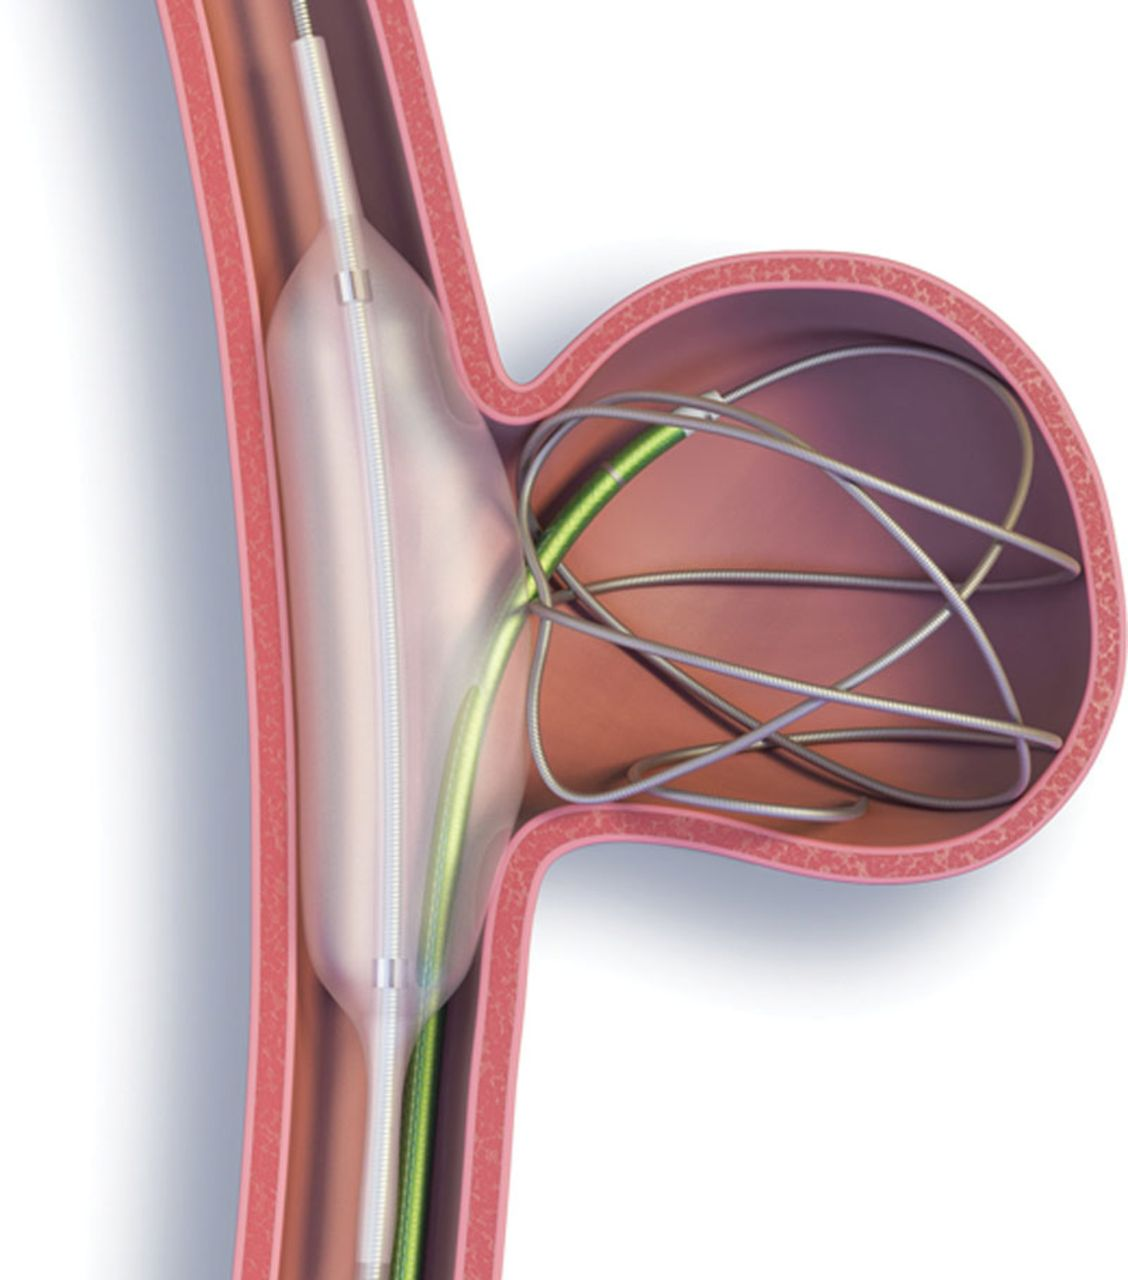
\includegraphics[width=0.5\textwidth, angle=90, origin=c]{figures/aneurysm/ballooncoil.jpg}
    \caption[An illustration of an aneurysm treated with balloon-assisted coiling]{An illustration of an aneurysm treated with balloon-assisted coiling \cite[Figure 2]{imaging}.}
    \label{fig:ballooncoil}
\end{figure}

Generally, the shape of the coil is known before it is inserted into the blood vessel. However, it remains difficult to determine the exact geometry of the coil within the aneurysm itself once it is inserted, even with modern imaging techniques \cite{imaging}, as we can see in Figure \ref{fig:coilinaneurysm}. This is due to a number of reasons: the coils themselves are often very small, yet geometrically complex and once inserted into the aneurysm, they are often distributed unpredictably, as described by Morales et al. in \cite{Morales2011}. 

\begin{figure}[!htb]
    \centering
    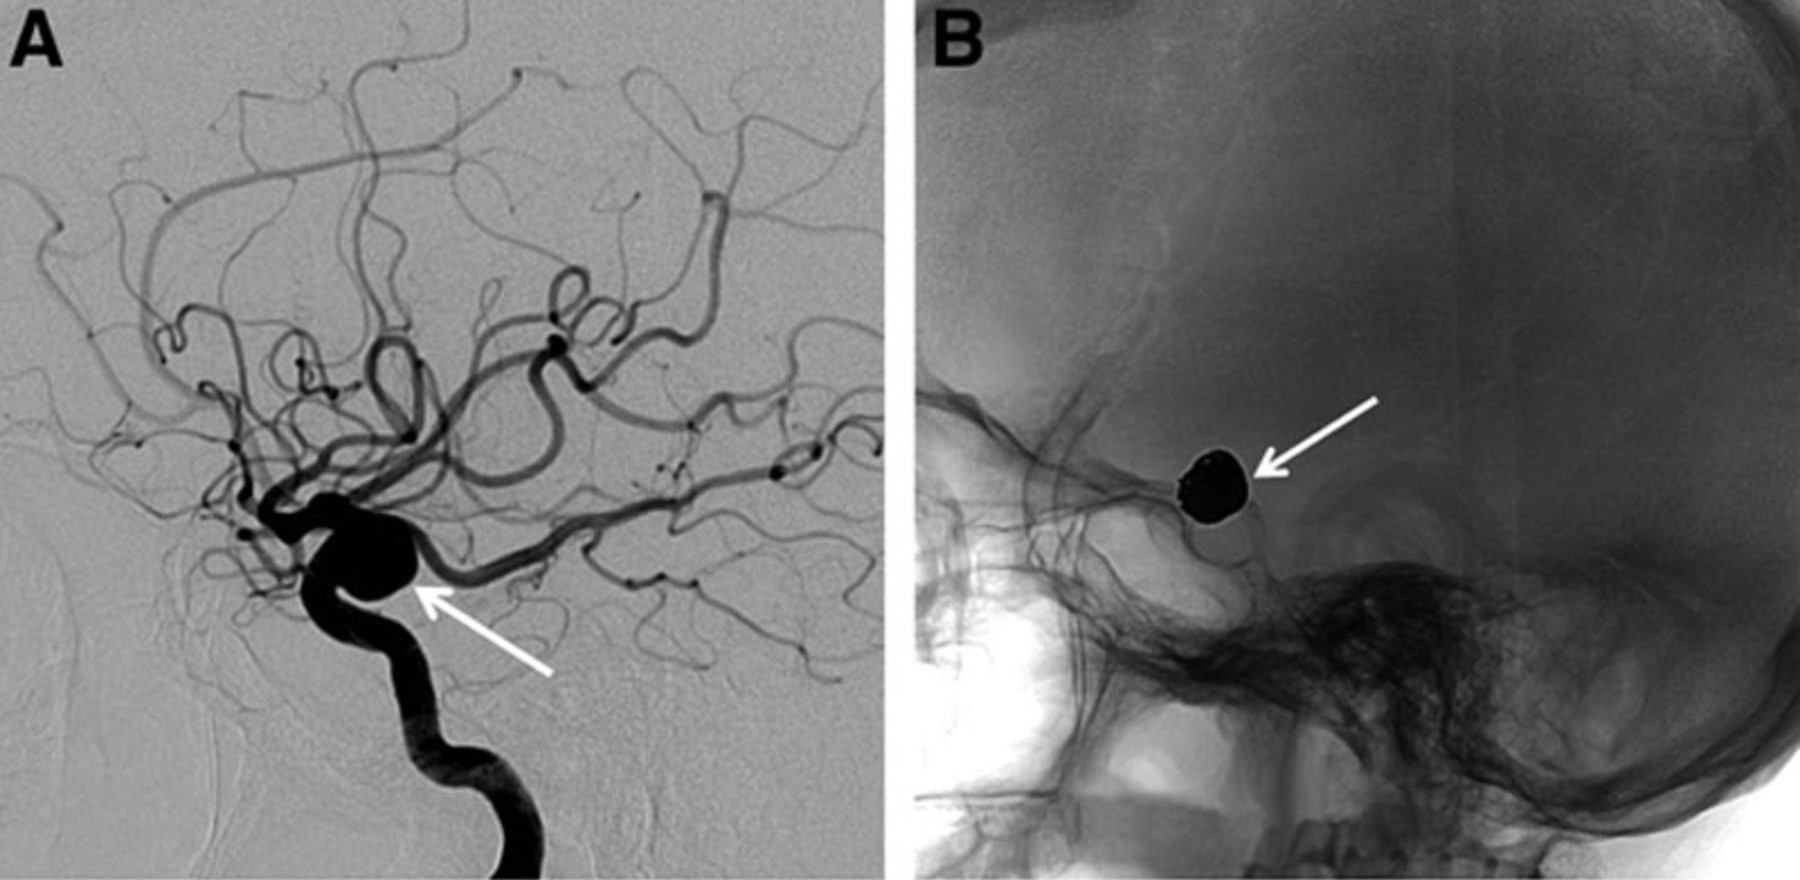
\includegraphics[width=0.7\textwidth]{figures/aneurysm/aneurysmcoil.jpg}
    % 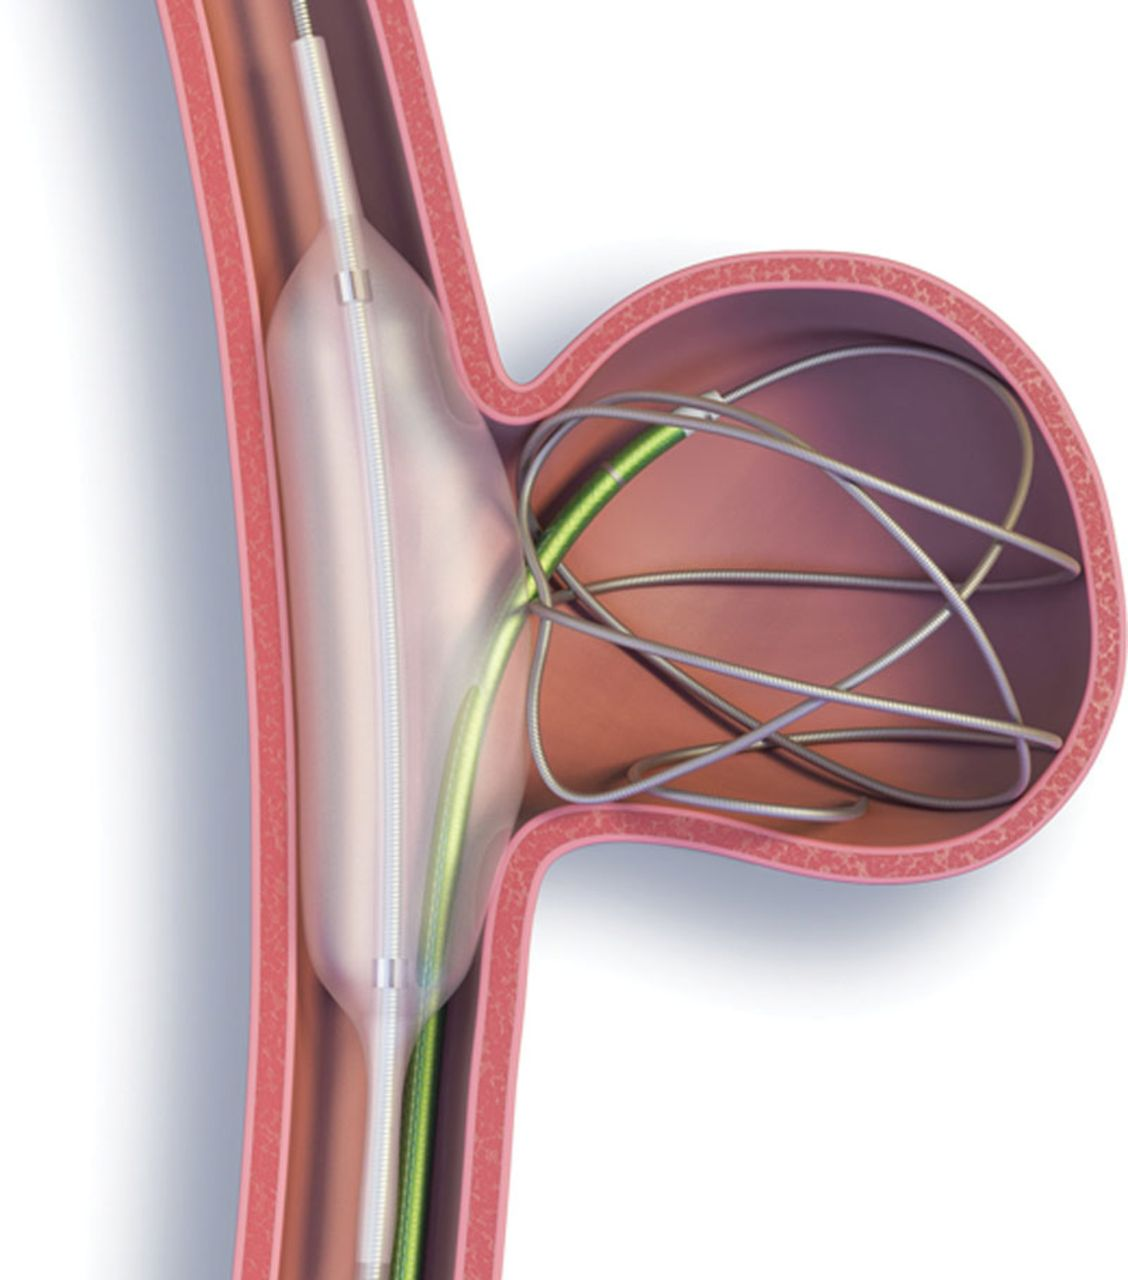
\includegraphics[width=0.45\textwidth, angle=90, origin=c]{figures/aneurysm/ballooncoil.jpg}
    \caption[A medical image of an aneurysm]{A medical image of an aneurysm - the arrow in \textbf{A} points to an aneurysm, the arrow in \textbf{B} indicates an aneurysm that has been treated by a coil \cite[Figure 1]{imaging}.}
    \label{fig:coilinaneurysm}
\end{figure}
\newpage
Researchers have conducted studies to simulate the blood flow dynamics in coiled aneurysms, where they have modelled coils explicitly using spheres \cite{BYUN2004} as well as modelled the aneurysms as porous media \cite{kakalis2008}. In line with what we have been doing so far, we can model the aneurysm as a porous medium by treating the coil as the $\alpha$-phase and blood as the $\beta$-phase.

% Studies have been conducted in order to simulate the blood flow dynamics in coiled aneurysms, where researchers have both modelled the coils explicitly, using spheres for instance \cite{BYUN2004}, and modelled the aneurysms as porous media \cite{kakalis2008}.

There are many assumptions that must be made in order to do this. For instance, blood flow is typically non-Newtonian due to the high volume of red blood cells \cite{MORALES2013} but for simplicity, we assume the fluid is Newtonian and thus, the viscosity of the fluid is constant. One could also argue that the elasticity of the coil could have an effect on the fluid flow, but the coils are packed tightly into the aneurysm itself. For that reason, we will assume the coil within the aneurysm, and therefore the porous medium used to model the aneurysm, is rigid and isotropic.

% Accordingly, we can model the aneurysm as a porous medium. 

% We consider the case where the aneurysm has been treated with the insertion of a coil. As mentioned in Chapter \ref{chap:1}, it is difficult to determine the exact geometry of the coil within the aneurysm once inserted, allowing us to model the aneurysm as a porous medium, assuming the porous medium is rigid and blood is a Newtonian fluid.

% Finally, we will collate what we have done in the previous chapters, as well as the benchmark cases to model blood flow through an aneurysm. We consider the case where the aneurysm has been treated with a coil. The exact geometry of this coil within the aneurysm is often unknown, although its configuration and effect on the dynamics of blood flow remains a topic of interest to researchers. \todo{check link } Therefore, the region formed by the aneurysm can be modelled as a porous medium. As mentioned in Chapter \ref{chap:1}, we assume this porous medium is rigid and that blood is a Newtonian fluid.

% We therefore model this region as a porous medium, as we have developed a model where we do not need to have the exact geometry of the coil within the aneurysm to simulate the flow.

We consider the situation illustrated in Figure \ref{fig:an_sketch}, where we have a circular deformation of the blood vessel. The radius of this circle is labelled by $r$ and the width of the blood vessel is labelled by $L$. Note that $H$ is the length of the blood vessel that we will be modelling.

\begin{figure}[!htb]
\centering
\begin{tikzpicture}[thick,scale=1.1, every node/.style={scale=1}, >={Latex[length=1.5mm, width=1mm]}]
    \draw (0, -0.5) -- (6, -0.5);
    \draw (0, 1) -- (2.4, 1);
    \draw (3.6, 1) -- (6, 1);
    \draw (3.6, 1) arc[start angle = -53.1, end angle = 233.1, radius = 1];
    % \draw [gray, thin, dashed] (3.88, 1) arc[start angle = -30, end angle = -150, radius = 1];
    \begin{scope}
    \path[clip] (3,1.8) circle (1);
    \fill[thick, pattern=north east lines, pattern color=red] (2,1) -- (4,1) -- (4,3) -- (2,3) -- cycle;
    \end{scope}
    \draw[black, <-] (1, -0.5) -- (1, 0);
    \draw[black, ->] (1, 0.5) -- (1, 1);
    \node at (1, 0.25) {$L$};
    \draw[black, <->] (3, 1.8) -- (2, 1.8);
    \node at (2.5, 2) {$r$};
    \draw[black, <-] (0, -0.75) -- (2.75, -0.75);
    \draw[black, ->] (3.25, -0.75) -- (6, -0.75);
    \node at (3, -0.75) {$H$};
\end{tikzpicture}
\caption{A diagram of an aneurysm on a blood vessel.} \label{fig:an_sketch}
\end{figure}

% We consider the situation illustrated in Figure \ref{fig:an_sketch}, where we have a circular deformation of the blood vessel. The radius of this circle is labelled by $r$ and the width of the blood vessel is labelled by $L$. Note that $H$ is the length of the blood vessel that we will be modelling.

To model the shape of the aneurysm, we will create a \textbf{mask}, or an array consisting of the values 0 and 1 only. We create both a mask for the outline of the aneurysm, which we will refer to as the \textit{mask}, and a mask containing all the lattice points within the blood vessel and aneurysm, which we will refer to as the \emph{inner mask}, as shown in Figure \ref{fig:mask}. The code for this is provided in Appendix \ref{sec:B.3}.

\begin{figure}[!htb]
    \centering
    \begin{tabular}{p{0.45\textwidth}p{0.45\textwidth}}
       % This file was created with tikzplotlib v0.10.1.
\begin{tikzpicture}
\pgfplotsset{%
    width=0.4\textwidth,
    height=0.4\textwidth
}
\definecolor{darkgray176}{RGB}{176,176,176}

\begin{axis}[
colorbar,
colorbar style={ylabel={}},
colormap={mymap}{[1pt]
  rgb(0pt)=(0.501960784313725,0,0.149019607843137);
  rgb(1pt)=(0.741176470588235,0,0.149019607843137);
  rgb(2pt)=(0.890196078431372,0.101960784313725,0.109803921568627);
  rgb(3pt)=(0.988235294117647,0.305882352941176,0.164705882352941);
  rgb(4pt)=(0.992156862745098,0.552941176470588,0.235294117647059);
  rgb(5pt)=(0.996078431372549,0.698039215686274,0.298039215686275);
  rgb(6pt)=(0.996078431372549,0.850980392156863,0.462745098039216);
  rgb(7pt)=(1,0.929411764705882,0.627450980392157);
  rgb(8pt)=(1,1,0.8)
},
point meta max=1,
point meta min=0,
tick align=outside,
tick pos=left,
x grid style={darkgray176},
xmin=-0.5, xmax=79.5,
xtick style={color=black},
y grid style={darkgray176},
ymin=-0.5, ymax=79.5,
ytick style={color=black}
]
\addplot graphics [includegraphics cmd=\pgfimage,xmin=-0.5, xmax=79.5, ymin=-0.5, ymax=79.5] {figures/aneurysm/mask-000.png};
\end{axis}

\end{tikzpicture}
  & % This file was created with tikzplotlib v0.10.1.
\begin{tikzpicture}
\pgfplotsset{%
    width=0.4\textwidth,
    height=0.4\textwidth
}
\definecolor{darkgray176}{RGB}{176,176,176}

\begin{axis}[
colorbar,
colorbar style={ylabel={}},
colormap={mymap}{[1pt]
  rgb(0pt)=(0.501960784313725,0,0.149019607843137);
  rgb(1pt)=(0.741176470588235,0,0.149019607843137);
  rgb(2pt)=(0.890196078431372,0.101960784313725,0.109803921568627);
  rgb(3pt)=(0.988235294117647,0.305882352941176,0.164705882352941);
  rgb(4pt)=(0.992156862745098,0.552941176470588,0.235294117647059);
  rgb(5pt)=(0.996078431372549,0.698039215686274,0.298039215686275);
  rgb(6pt)=(0.996078431372549,0.850980392156863,0.462745098039216);
  rgb(7pt)=(1,0.929411764705882,0.627450980392157);
  rgb(8pt)=(1,1,0.8)
},
point meta max=1,
point meta min=0,
tick align=outside,
tick pos=left,
x grid style={darkgray176},
xmin=-0.5, xmax=79.5,
xtick style={color=black},
y grid style={darkgray176},
ymin=-0.5, ymax=79.5,
ytick style={color=black}
]
\addplot graphics [includegraphics cmd=\pgfimage,xmin=-0.5, xmax=79.5, ymin=-0.5, ymax=79.5] {figures/aneurysm/inner_mask-000.png};
\end{axis}

\end{tikzpicture}

       % A mask of points in the shape of an aneurysm  & A mask of points in the shape of an aneurysm including the points within the blood vessel
    \end{tabular}
    \vspace{-5mm}
    \caption[Masks of the aneurysm]{The \emph{mask} and \emph{inner mask} of the aneurysm - this gives the lattice points that form the outline of an aneurysm and all lattice points within the blood vessel and aneurysm.} \label{fig:mask}
\end{figure}

% To model the shape of the aneurysm, we will create a mask, or an array consisting of the values 0 and 1 only. We create both a mask for the outline of the aneurysm, which we will refer to as the \textit{mask}, and a mask containing all the lattice points within the blood vessel and aneurysm, which we will refer to as the \emph{inner mask}, as shown in Figure \ref{fig:mask}. The code for this is provided in Appendix \ref{sec:B.3}.
\newpage
As before, the domain has dimensions $80\times80$ and relaxation time $\tau=0.8$. To initialise, the velocity is set to zero and the density is set to 1.0 at each lattice node. The distribution function $f_k$ is also set to $f_k^{\mathrm{eq}}$ at $t=0$. As we are modelling regions of various porosities, we set
\vspace{-1mm}
\begin{align}
    \varepsilon_\beta &= 
    \begin{cases}
        1.0 \quad & \textit{inner mask} = 1, \\
        0.5 & \textit{inner mask} = 1 \quad \text{and} \quad y > L, \\
        0.1 & \text{otherwise},
    \end{cases} \\
    \mathrm{Da} &=
    \begin{cases}
        10^6 & \textit{inner mask} = 1, \\
        10^{-3} \text{ }& \textit{inner mask} = 1 \quad \text{and} \quad y > L, \\
        10^{-6} & \text{otherwise},
    \end{cases}
\end{align}
noting that the region where $y>L$ indicates the aneurysm where there is a deformation in the blood vessel. We model blood flow as a pure fluid flow and the outside region, or the region that is neither the aneurysm nor the blood vessel, as `almost solid'. Generally, we will ignore this outside region.

According to section 14.2.6 of \cite{reynblood}, the Reynolds number is 500 for a typical artery and 400 for a typical vein. As such, we will take the Reynolds number to be 450 for these flows. 

As there are no moving boundaries in this flow, the fluid flow is driven by a constant force, which we have to specify. We take $\mathbf{g}=(g_x,0)$ with $g_x=10^{-4}$ to avoid overflow errors but the value of this does not matter as we are more interested in the steady-state flow. 

Initially, we consider the flow where the porosity within the aneurysm is 0.5, with a Darcy number $10^{-3}$. To account for the shape of the aneurysm, we employ the half-way bounce-back scheme on every lattice point where the mask is equal to 1, i.e. the outline of the aneurysm is considered to be solid. Figure \ref{fig:an_hbb} gives the implementation of this in Python.

\begin{figure}[!htb]{\small
\begin{mdframed}[backgroundcolor=red!10, linecolor=red!10]
\begin{minted}{python}
    for k in range(ndir):
        for i in range(nx):
            for j in range(ny):
                if mask[i,j] == 1:
                    fold[k, i, j] = f[k_[k], i, j]
\end{minted}
\end{mdframed}
}
\caption[Python implementation of the half-way bounce-back scheme on aneurysm]{Implementation of the half-way bounce-back scheme on every point in the mask equal to 1, note that {\fontfamily{cmtt}\selectfont k\_} represents $k'$ given by Table \ref{table:d2q9}.} \label{fig:an_hbb}
\end{figure}
\newpage
This simulation is run until the flow is steady, that is, the difference between the velocity in the current time step and the previous time step is constant. As such, we run all the simulations in this section for 10,000 time steps or more. 
\begin{figure}[!hbt]
    \centering
    \begin{tabular}{c c}
    % This file was created with tikzplotlib v0.10.1.
\begin{tikzpicture}
\pgfplotsset{%
    width=0.4\textwidth,
    height=0.4\textwidth
}
\definecolor{darkgray176}{RGB}{176,176,176}

\begin{axis}[
colorbar,
colorbar style={ylabel={}},
colormap={mymap}{[1pt]
  rgb(0pt)=(0.501960784313725,0,0.149019607843137);
  rgb(1pt)=(0.741176470588235,0,0.149019607843137);
  rgb(2pt)=(0.890196078431372,0.101960784313725,0.109803921568627);
  rgb(3pt)=(0.988235294117647,0.305882352941176,0.164705882352941);
  rgb(4pt)=(0.992156862745098,0.552941176470588,0.235294117647059);
  rgb(5pt)=(0.996078431372549,0.698039215686274,0.298039215686275);
  rgb(6pt)=(0.996078431372549,0.850980392156863,0.462745098039216);
  rgb(7pt)=(1,0.929411764705882,0.627450980392157);
  rgb(8pt)=(1,1,0.8)
},
point meta max=0.0939234317467123,
point meta min=1.27672414769124e-14,
tick align=outside,
tick pos=left,
x grid style={darkgray176},
xlabel={x},
xmin=-0.5, xmax=79.5,
xtick style={color=black},
y grid style={darkgray176},
ylabel={y},
ymin=-0.5, ymax=79.5,
ytick style={color=black}
]
\addplot graphics [includegraphics cmd=\pgfimage,xmin=-0.5, xmax=79.5, ymin=-0.5, ymax=79.5] {figures/aneurysm/porous0.5-000.png};
\end{axis}

\end{tikzpicture}
  &  % This file was created with tikzplotlib v0.10.1.
\begin{tikzpicture}
\pgfplotsset{%
    width=0.4\textwidth,
    height=0.4\textwidth
}
\definecolor{darkgray176}{RGB}{176,176,176}

\begin{axis}[
colorbar,
colorbar style={ylabel={}},
colormap={mymap}{[1pt]
  rgb(0pt)=(0.501960784313725,0,0.149019607843137);
  rgb(1pt)=(0.741176470588235,0,0.149019607843137);
  rgb(2pt)=(0.890196078431372,0.101960784313725,0.109803921568627);
  rgb(3pt)=(0.988235294117647,0.305882352941176,0.164705882352941);
  rgb(4pt)=(0.992156862745098,0.552941176470588,0.235294117647059);
  rgb(5pt)=(0.996078431372549,0.698039215686274,0.298039215686275);
  rgb(6pt)=(0.996078431372549,0.850980392156863,0.462745098039216);
  rgb(7pt)=(1,0.929411764705882,0.627450980392157);
  rgb(8pt)=(1,1,0.8)
},
point meta max=0.005,
point meta min=0,
tick align=outside,
tick pos=left,
x grid style={darkgray176},
xlabel={x},
xmin=-0.5, xmax=79.5,
xtick style={color=black},
y grid style={darkgray176},
ylabel={y},
ymin=-0.5, ymax=79.5,
ytick style={color=black}
]
\addplot graphics [includegraphics cmd=\pgfimage,xmin=-0.5, xmax=79.5, ymin=-0.5, ymax=79.5] {figures/aneurysm/porousDa3-000.png};
\end{axis}

\end{tikzpicture}
\\
    (i) & (ii)
    \end{tabular}
    % % This file was created with tikzplotlib v0.10.1.
\begin{tikzpicture}
\pgfplotsset{%
    width=0.4\textwidth,
    height=0.4\textwidth
}
\definecolor{darkgray176}{RGB}{176,176,176}

\begin{axis}[
colorbar,
colorbar style={ylabel={}},
colormap={mymap}{[1pt]
  rgb(0pt)=(0.501960784313725,0,0.149019607843137);
  rgb(1pt)=(0.741176470588235,0,0.149019607843137);
  rgb(2pt)=(0.890196078431372,0.101960784313725,0.109803921568627);
  rgb(3pt)=(0.988235294117647,0.305882352941176,0.164705882352941);
  rgb(4pt)=(0.992156862745098,0.552941176470588,0.235294117647059);
  rgb(5pt)=(0.996078431372549,0.698039215686274,0.298039215686275);
  rgb(6pt)=(0.996078431372549,0.850980392156863,0.462745098039216);
  rgb(7pt)=(1,0.929411764705882,0.627450980392157);
  rgb(8pt)=(1,1,0.8)
},
point meta max=0.0939234317467123,
point meta min=1.27672414769124e-14,
tick align=outside,
tick pos=left,
x grid style={darkgray176},
xlabel={x},
xmin=-0.5, xmax=79.5,
xtick style={color=black},
y grid style={darkgray176},
ylabel={y},
ymin=-0.5, ymax=79.5,
ytick style={color=black}
]
\addplot graphics [includegraphics cmd=\pgfimage,xmin=-0.5, xmax=79.5, ymin=-0.5, ymax=79.5] {figures/aneurysm/porous0.5-000.png};
\end{axis}

\end{tikzpicture}

    % % This file was created with tikzplotlib v0.10.1.
\begin{tikzpicture}
\pgfplotsset{%
    width=0.4\textwidth,
    height=0.4\textwidth
}
\definecolor{darkgray176}{RGB}{176,176,176}

\begin{axis}[
colorbar,
colorbar style={ylabel={}},
colormap={mymap}{[1pt]
  rgb(0pt)=(0.501960784313725,0,0.149019607843137);
  rgb(1pt)=(0.741176470588235,0,0.149019607843137);
  rgb(2pt)=(0.890196078431372,0.101960784313725,0.109803921568627);
  rgb(3pt)=(0.988235294117647,0.305882352941176,0.164705882352941);
  rgb(4pt)=(0.992156862745098,0.552941176470588,0.235294117647059);
  rgb(5pt)=(0.996078431372549,0.698039215686274,0.298039215686275);
  rgb(6pt)=(0.996078431372549,0.850980392156863,0.462745098039216);
  rgb(7pt)=(1,0.929411764705882,0.627450980392157);
  rgb(8pt)=(1,1,0.8)
},
point meta max=0.005,
point meta min=0,
tick align=outside,
tick pos=left,
x grid style={darkgray176},
xlabel={x},
xmin=-0.5, xmax=79.5,
xtick style={color=black},
y grid style={darkgray176},
ylabel={y},
ymin=-0.5, ymax=79.5,
ytick style={color=black}
]
\addplot graphics [includegraphics cmd=\pgfimage,xmin=-0.5, xmax=79.5, ymin=-0.5, ymax=79.5] {figures/aneurysm/porousDa3-000.png};
\end{axis}

\end{tikzpicture}

    \caption[Blood flow through an aneurysm with porosity $\varepsilon_\beta=0.5$ and $\mathrm{Da}=10^{-3}$]{Blood flow through an aneurysm with porosity $\varepsilon_\beta=0.5$ and $\mathrm{Da}=10^{-3}$ - (i) shows the full fluid flow through the blood vessel and aneurysm, (ii) is rescaled to show the fluid flow through the aneurysm.} \label{fig:an_0.5}
\end{figure}
\vspace{-5mm}

Figure \ref{fig:an_0.5} shows the blood flow within an aneurysm with porosity $\varepsilon_\beta=0.5$ and $\mathrm{Da}=10^{-3}$. Figure \ref{fig:an_0.5}(i) shows the full fluid flow through the blood vessel and aneurysm. As expected, the velocity of the fluid within the blood vessel is much higher than the fluid velocity within the aneurysm. As such, we rescaled the colour bar, restricting this to $[0,0.005]$, in order to see the fluid flow within the aneurysm better, as given by Figure \ref{fig:an_0.5}(ii). Here, we can see that the boundary of the aneurysm is rigid and there is no flow through this boundary. The velocity of the fluid is highest at the opening of the aneurysm and interestingly, there is a region of lower velocity at the centre of the aneurysm, suggesting the presence of a circular flow. 

We also consider the fluid flow when the flow through the aneurysm is that of a pure fluid, i.e. we take porosity within the aneurysm to be $\varepsilon_\beta=1.0$ and $\mathrm{Da}=10^{6}$, as shown in Figure \ref{fig:an_fluid}.

\begin{figure}[!htb]
    \centering
    \begin{tabular}{c c}
    % This file was created with tikzplotlib v0.10.1.
\begin{tikzpicture}
\pgfplotsset{%
    width=0.4\textwidth,
    height=0.4\textwidth
}
\definecolor{darkgray176}{RGB}{176,176,176}

\begin{axis}[
colorbar,
colorbar style={ylabel={}},
colormap={mymap}{[1pt]
  rgb(0pt)=(0.501960784313725,0,0.149019607843137);
  rgb(1pt)=(0.741176470588235,0,0.149019607843137);
  rgb(2pt)=(0.890196078431372,0.101960784313725,0.109803921568627);
  rgb(3pt)=(0.988235294117647,0.305882352941176,0.164705882352941);
  rgb(4pt)=(0.992156862745098,0.552941176470588,0.235294117647059);
  rgb(5pt)=(0.996078431372549,0.698039215686274,0.298039215686275);
  rgb(6pt)=(0.996078431372549,0.850980392156863,0.462745098039216);
  rgb(7pt)=(1,0.929411764705882,0.627450980392157);
  rgb(8pt)=(1,1,0.8)
},
point meta max=0.0940201043731662,
point meta min=2.24999749274148e-05,
tick align=outside,
tick pos=left,
x grid style={darkgray176},
xlabel={x},
xmin=-0.5, xmax=79.5,
xtick style={color=black},
y grid style={darkgray176},
ylabel={y},
ymin=-0.5, ymax=79.5,
ytick style={color=black}
]
\addplot graphics [includegraphics cmd=\pgfimage,xmin=-0.5, xmax=79.5, ymin=-0.5, ymax=79.5] {figures/aneurysm/fluid_full-000.png};
\end{axis}

\end{tikzpicture}
  &  % This file was created with tikzplotlib v0.10.1.
\begin{tikzpicture}
\pgfplotsset{%
    width=0.4\textwidth,
    height=0.4\textwidth
}
\definecolor{darkgray176}{RGB}{176,176,176}

\begin{axis}[
colorbar,
colorbar style={ylabel={}},
colormap={mymap}{[1pt]
  rgb(0pt)=(0.501960784313725,0,0.149019607843137);
  rgb(1pt)=(0.741176470588235,0,0.149019607843137);
  rgb(2pt)=(0.890196078431372,0.101960784313725,0.109803921568627);
  rgb(3pt)=(0.988235294117647,0.305882352941176,0.164705882352941);
  rgb(4pt)=(0.992156862745098,0.552941176470588,0.235294117647059);
  rgb(5pt)=(0.996078431372549,0.698039215686274,0.298039215686275);
  rgb(6pt)=(0.996078431372549,0.850980392156863,0.462745098039216);
  rgb(7pt)=(1,0.929411764705882,0.627450980392157);
  rgb(8pt)=(1,1,0.8)
},
point meta max=0.005,
point meta min=0,
tick align=outside,
tick pos=left,
x grid style={darkgray176},
xlabel={x},
xmin=-0.5, xmax=79.5,
xtick style={color=black},
y grid style={darkgray176},
ylabel={y},
ymin=-0.5, ymax=79.5,
ytick style={color=black}
]
\addplot graphics [includegraphics cmd=\pgfimage,xmin=-0.5, xmax=79.5, ymin=-0.5, ymax=79.5] {figures/aneurysm/fluid-000.png};
\end{axis}

\end{tikzpicture}
\\
    (i) & (ii) 
    \end{tabular}
    % % This file was created with tikzplotlib v0.10.1.
\begin{tikzpicture}
\pgfplotsset{%
    width=0.4\textwidth,
    height=0.4\textwidth
}
\definecolor{darkgray176}{RGB}{176,176,176}

\begin{axis}[
colorbar,
colorbar style={ylabel={}},
colormap={mymap}{[1pt]
  rgb(0pt)=(0.501960784313725,0,0.149019607843137);
  rgb(1pt)=(0.741176470588235,0,0.149019607843137);
  rgb(2pt)=(0.890196078431372,0.101960784313725,0.109803921568627);
  rgb(3pt)=(0.988235294117647,0.305882352941176,0.164705882352941);
  rgb(4pt)=(0.992156862745098,0.552941176470588,0.235294117647059);
  rgb(5pt)=(0.996078431372549,0.698039215686274,0.298039215686275);
  rgb(6pt)=(0.996078431372549,0.850980392156863,0.462745098039216);
  rgb(7pt)=(1,0.929411764705882,0.627450980392157);
  rgb(8pt)=(1,1,0.8)
},
point meta max=0.0940201043731662,
point meta min=2.24999749274148e-05,
tick align=outside,
tick pos=left,
x grid style={darkgray176},
xlabel={x},
xmin=-0.5, xmax=79.5,
xtick style={color=black},
y grid style={darkgray176},
ylabel={y},
ymin=-0.5, ymax=79.5,
ytick style={color=black}
]
\addplot graphics [includegraphics cmd=\pgfimage,xmin=-0.5, xmax=79.5, ymin=-0.5, ymax=79.5] {figures/aneurysm/fluid_full-000.png};
\end{axis}

\end{tikzpicture}

    % % This file was created with tikzplotlib v0.10.1.
\begin{tikzpicture}
\pgfplotsset{%
    width=0.4\textwidth,
    height=0.4\textwidth
}
\definecolor{darkgray176}{RGB}{176,176,176}

\begin{axis}[
colorbar,
colorbar style={ylabel={}},
colormap={mymap}{[1pt]
  rgb(0pt)=(0.501960784313725,0,0.149019607843137);
  rgb(1pt)=(0.741176470588235,0,0.149019607843137);
  rgb(2pt)=(0.890196078431372,0.101960784313725,0.109803921568627);
  rgb(3pt)=(0.988235294117647,0.305882352941176,0.164705882352941);
  rgb(4pt)=(0.992156862745098,0.552941176470588,0.235294117647059);
  rgb(5pt)=(0.996078431372549,0.698039215686274,0.298039215686275);
  rgb(6pt)=(0.996078431372549,0.850980392156863,0.462745098039216);
  rgb(7pt)=(1,0.929411764705882,0.627450980392157);
  rgb(8pt)=(1,1,0.8)
},
point meta max=0.005,
point meta min=0,
tick align=outside,
tick pos=left,
x grid style={darkgray176},
xlabel={x},
xmin=-0.5, xmax=79.5,
xtick style={color=black},
y grid style={darkgray176},
ylabel={y},
ymin=-0.5, ymax=79.5,
ytick style={color=black}
]
\addplot graphics [includegraphics cmd=\pgfimage,xmin=-0.5, xmax=79.5, ymin=-0.5, ymax=79.5] {figures/aneurysm/fluid-000.png};
\end{axis}

\end{tikzpicture}

    \caption[Blood flow through an aneurysm as a pure fluid]{Blood flow through an aneurysm with porosity $\varepsilon_\beta=1.0$ and $\mathrm{Da}=10^{6}$ - (i) shows the full fluid flow through the blood vessel and aneurysm, (ii) is rescaled to show the fluid flow through the aneurysm.} \label{fig:an_fluid}
\end{figure}

% We also consider the fluid flow when the flow through the aneurysm is that of a pure fluid, i.e. we take porosity within the aneurysm to be $\varepsilon_\beta=1.0$ and $\mathrm{Da}=10^{6}$, as shown in Figure \ref{fig:an_fluid}.

Like Figure \ref{fig:an_0.5}, Figure \ref{fig:an_fluid}(i) shows the full fluid flow through the blood vessel and aneurysm, and the colour bar has been restricted in order to see the fluid flow within the aneurysm better. As we can see, the fluid flow through this aneurysm is much higher than if it had been treated with a coil, but the direction of the flow is similar, with the velocity of the fluid being highest at the opening, and with a region of lower velocity at the centre of the aneurysm. It is also worth noting that Figure \ref{fig:an_0.5}(i) and Figure \ref{fig:an_fluid}(i) are indistinguishable, and consequently, the full fluid flows will not be shown moving forward.

% As the full fluid flows are indistinguishable for different porosities and Darcy numbers, these flows will not be shown moving forward.

% We now vary the Darcy numbers for constant porosity, as shown in Figure \ref{fig:an_Da}. 
Figure \ref{fig:an_Da} shows the fluid flows when porosity is constant at $\varepsilon_\beta = 0.5$ and the Darcy number is changed, taking values from $\mathrm{Da} = 10^{-6}$ to $\mathrm{Da} = 10^{-1}$. From the figure, we can see that as the Darcy number is increased, which in turn increases the permeability of the aneurysm, it becomes easier for the fluid to flow through the aneurysm. As a result, the velocity of the blood within the aneurysm also increases.

\begin{figure}[p]
    \centering
    \begin{tabular}{c c}
    % This file was created with tikzplotlib v0.10.1.
\begin{tikzpicture}
\pgfplotsset{%
    width=0.4\textwidth,
    height=0.4\textwidth
}
\definecolor{darkgray176}{RGB}{176,176,176}

\begin{axis}[
colorbar,
colorbar style={ylabel={}},
colormap={mymap}{[1pt]
  rgb(0pt)=(0.501960784313725,0,0.149019607843137);
  rgb(1pt)=(0.741176470588235,0,0.149019607843137);
  rgb(2pt)=(0.890196078431372,0.101960784313725,0.109803921568627);
  rgb(3pt)=(0.988235294117647,0.305882352941176,0.164705882352941);
  rgb(4pt)=(0.992156862745098,0.552941176470588,0.235294117647059);
  rgb(5pt)=(0.996078431372549,0.698039215686274,0.298039215686275);
  rgb(6pt)=(0.996078431372549,0.850980392156863,0.462745098039216);
  rgb(7pt)=(1,0.929411764705882,0.627450980392157);
  rgb(8pt)=(1,1,0.8)
},
point meta max=0.005,
point meta min=0,
tick align=outside,
tick pos=left,
x grid style={darkgray176},
xlabel={x},
xmin=-0.5, xmax=79.5,
xtick style={color=black},
y grid style={darkgray176},
ylabel={y},
ymin=-0.5, ymax=79.5,
ytick style={color=black}
]
\addplot graphics [includegraphics cmd=\pgfimage,xmin=-0.5, xmax=79.5, ymin=-0.5, ymax=79.5] {figures/aneurysm/porousDa6-000.png};
\end{axis}

\end{tikzpicture}
  &  % This file was created with tikzplotlib v0.10.1.
\begin{tikzpicture}
\pgfplotsset{%
    width=0.4\textwidth,
    height=0.4\textwidth
}
\definecolor{darkgray176}{RGB}{176,176,176}

\begin{axis}[
colorbar,
colorbar style={ylabel={}},
colormap={mymap}{[1pt]
  rgb(0pt)=(0.501960784313725,0,0.149019607843137);
  rgb(1pt)=(0.741176470588235,0,0.149019607843137);
  rgb(2pt)=(0.890196078431372,0.101960784313725,0.109803921568627);
  rgb(3pt)=(0.988235294117647,0.305882352941176,0.164705882352941);
  rgb(4pt)=(0.992156862745098,0.552941176470588,0.235294117647059);
  rgb(5pt)=(0.996078431372549,0.698039215686274,0.298039215686275);
  rgb(6pt)=(0.996078431372549,0.850980392156863,0.462745098039216);
  rgb(7pt)=(1,0.929411764705882,0.627450980392157);
  rgb(8pt)=(1,1,0.8)
},
point meta max=0.005,
point meta min=0,
tick align=outside,
tick pos=left,
x grid style={darkgray176},
xlabel={x},
xmin=-0.5, xmax=79.5,
xtick style={color=black},
y grid style={darkgray176},
ylabel={y},
ymin=-0.5, ymax=79.5,
ytick style={color=black}
]
\addplot graphics [includegraphics cmd=\pgfimage,xmin=-0.5, xmax=79.5, ymin=-0.5, ymax=79.5] {figures/aneurysm/porousDa5-000.png};
\end{axis}

\end{tikzpicture}
\\
    (i) $\mathrm{Da}=10^{-6}$ & (ii) $\mathrm{Da}=10^{-5}$ \\
    % This file was created with tikzplotlib v0.10.1.
\begin{tikzpicture}
\pgfplotsset{%
    width=0.4\textwidth,
    height=0.4\textwidth
}
\definecolor{darkgray176}{RGB}{176,176,176}

\begin{axis}[
colorbar,
colorbar style={ylabel={}},
colormap={mymap}{[1pt]
  rgb(0pt)=(0.501960784313725,0,0.149019607843137);
  rgb(1pt)=(0.741176470588235,0,0.149019607843137);
  rgb(2pt)=(0.890196078431372,0.101960784313725,0.109803921568627);
  rgb(3pt)=(0.988235294117647,0.305882352941176,0.164705882352941);
  rgb(4pt)=(0.992156862745098,0.552941176470588,0.235294117647059);
  rgb(5pt)=(0.996078431372549,0.698039215686274,0.298039215686275);
  rgb(6pt)=(0.996078431372549,0.850980392156863,0.462745098039216);
  rgb(7pt)=(1,0.929411764705882,0.627450980392157);
  rgb(8pt)=(1,1,0.8)
},
point meta max=0.005,
point meta min=0,
tick align=outside,
tick pos=left,
x grid style={darkgray176},
xlabel={x},
xmin=-0.5, xmax=79.5,
xtick style={color=black},
y grid style={darkgray176},
ylabel={y},
ymin=-0.5, ymax=79.5,
ytick style={color=black}
]
\addplot graphics [includegraphics cmd=\pgfimage,xmin=-0.5, xmax=79.5, ymin=-0.5, ymax=79.5] {figures/aneurysm/porousDa4-000.png};
\end{axis}

\end{tikzpicture}
  &  % This file was created with tikzplotlib v0.10.1.
\begin{tikzpicture}
\pgfplotsset{%
    width=0.4\textwidth,
    height=0.4\textwidth
}
\definecolor{darkgray176}{RGB}{176,176,176}

\begin{axis}[
colorbar,
colorbar style={ylabel={}},
colormap={mymap}{[1pt]
  rgb(0pt)=(0.501960784313725,0,0.149019607843137);
  rgb(1pt)=(0.741176470588235,0,0.149019607843137);
  rgb(2pt)=(0.890196078431372,0.101960784313725,0.109803921568627);
  rgb(3pt)=(0.988235294117647,0.305882352941176,0.164705882352941);
  rgb(4pt)=(0.992156862745098,0.552941176470588,0.235294117647059);
  rgb(5pt)=(0.996078431372549,0.698039215686274,0.298039215686275);
  rgb(6pt)=(0.996078431372549,0.850980392156863,0.462745098039216);
  rgb(7pt)=(1,0.929411764705882,0.627450980392157);
  rgb(8pt)=(1,1,0.8)
},
point meta max=0.005,
point meta min=0,
tick align=outside,
tick pos=left,
x grid style={darkgray176},
xlabel={x},
xmin=-0.5, xmax=79.5,
xtick style={color=black},
y grid style={darkgray176},
ylabel={y},
ymin=-0.5, ymax=79.5,
ytick style={color=black}
]
\addplot graphics [includegraphics cmd=\pgfimage,xmin=-0.5, xmax=79.5, ymin=-0.5, ymax=79.5] {figures/aneurysm/porousDa3-000.png};
\end{axis}

\end{tikzpicture}
\\
    (iii) $\mathrm{Da}=10^{-4}$ & (iv) $\mathrm{Da}=10^{-3}$ \\
    % This file was created with tikzplotlib v0.10.1.
\begin{tikzpicture}
\pgfplotsset{%
    width=0.4\textwidth,
    height=0.4\textwidth
}
\definecolor{darkgray176}{RGB}{176,176,176}

\begin{axis}[
colorbar,
colorbar style={ylabel={}},
colormap={mymap}{[1pt]
  rgb(0pt)=(0.501960784313725,0,0.149019607843137);
  rgb(1pt)=(0.741176470588235,0,0.149019607843137);
  rgb(2pt)=(0.890196078431372,0.101960784313725,0.109803921568627);
  rgb(3pt)=(0.988235294117647,0.305882352941176,0.164705882352941);
  rgb(4pt)=(0.992156862745098,0.552941176470588,0.235294117647059);
  rgb(5pt)=(0.996078431372549,0.698039215686274,0.298039215686275);
  rgb(6pt)=(0.996078431372549,0.850980392156863,0.462745098039216);
  rgb(7pt)=(1,0.929411764705882,0.627450980392157);
  rgb(8pt)=(1,1,0.8)
},
point meta max=0.005,
point meta min=0,
tick align=outside,
tick pos=left,
x grid style={darkgray176},
xlabel={x},
xmin=-0.5, xmax=79.5,
xtick style={color=black},
y grid style={darkgray176},
ylabel={y},
ymin=-0.5, ymax=79.5,
ytick style={color=black}
]
\addplot graphics [includegraphics cmd=\pgfimage,xmin=-0.5, xmax=79.5, ymin=-0.5, ymax=79.5] {figures/aneurysm/porousDa2-000.png};
\end{axis}

\end{tikzpicture}
  &  % This file was created with tikzplotlib v0.10.1.
\begin{tikzpicture}
\pgfplotsset{%
    width=0.4\textwidth,
    height=0.4\textwidth
}
\definecolor{darkgray176}{RGB}{176,176,176}

\begin{axis}[
colorbar,
colorbar style={ylabel={}},
colormap={mymap}{[1pt]
  rgb(0pt)=(0.501960784313725,0,0.149019607843137);
  rgb(1pt)=(0.741176470588235,0,0.149019607843137);
  rgb(2pt)=(0.890196078431372,0.101960784313725,0.109803921568627);
  rgb(3pt)=(0.988235294117647,0.305882352941176,0.164705882352941);
  rgb(4pt)=(0.992156862745098,0.552941176470588,0.235294117647059);
  rgb(5pt)=(0.996078431372549,0.698039215686274,0.298039215686275);
  rgb(6pt)=(0.996078431372549,0.850980392156863,0.462745098039216);
  rgb(7pt)=(1,0.929411764705882,0.627450980392157);
  rgb(8pt)=(1,1,0.8)
},
point meta max=0.005,
point meta min=0,
tick align=outside,
tick pos=left,
x grid style={darkgray176},
xlabel={x},
xmin=-0.5, xmax=79.5,
xtick style={color=black},
y grid style={darkgray176},
ylabel={y},
ymin=-0.5, ymax=79.5,
ytick style={color=black}
]
\addplot graphics [includegraphics cmd=\pgfimage,xmin=-0.5, xmax=79.5, ymin=-0.5, ymax=79.5] {figures/aneurysm/porousDa1-000.png};
\end{axis}

\end{tikzpicture}
\\
    (v) $\mathrm{Da}=10^{-2}$ & (vi) $\mathrm{Da}=10^{-1}$
    \end{tabular}
    % % This file was created with tikzplotlib v0.10.1.
\begin{tikzpicture}
\pgfplotsset{%
    width=0.4\textwidth,
    height=0.4\textwidth
}
\definecolor{darkgray176}{RGB}{176,176,176}

\begin{axis}[
colorbar,
colorbar style={ylabel={}},
colormap={mymap}{[1pt]
  rgb(0pt)=(0.501960784313725,0,0.149019607843137);
  rgb(1pt)=(0.741176470588235,0,0.149019607843137);
  rgb(2pt)=(0.890196078431372,0.101960784313725,0.109803921568627);
  rgb(3pt)=(0.988235294117647,0.305882352941176,0.164705882352941);
  rgb(4pt)=(0.992156862745098,0.552941176470588,0.235294117647059);
  rgb(5pt)=(0.996078431372549,0.698039215686274,0.298039215686275);
  rgb(6pt)=(0.996078431372549,0.850980392156863,0.462745098039216);
  rgb(7pt)=(1,0.929411764705882,0.627450980392157);
  rgb(8pt)=(1,1,0.8)
},
point meta max=0.005,
point meta min=0,
tick align=outside,
tick pos=left,
x grid style={darkgray176},
xlabel={x},
xmin=-0.5, xmax=79.5,
xtick style={color=black},
y grid style={darkgray176},
ylabel={y},
ymin=-0.5, ymax=79.5,
ytick style={color=black}
]
\addplot graphics [includegraphics cmd=\pgfimage,xmin=-0.5, xmax=79.5, ymin=-0.5, ymax=79.5] {figures/aneurysm/porousDa1-000.png};
\end{axis}

\end{tikzpicture}

    % % This file was created with tikzplotlib v0.10.1.
\begin{tikzpicture}
\pgfplotsset{%
    width=0.4\textwidth,
    height=0.4\textwidth
}
\definecolor{darkgray176}{RGB}{176,176,176}

\begin{axis}[
colorbar,
colorbar style={ylabel={}},
colormap={mymap}{[1pt]
  rgb(0pt)=(0.501960784313725,0,0.149019607843137);
  rgb(1pt)=(0.741176470588235,0,0.149019607843137);
  rgb(2pt)=(0.890196078431372,0.101960784313725,0.109803921568627);
  rgb(3pt)=(0.988235294117647,0.305882352941176,0.164705882352941);
  rgb(4pt)=(0.992156862745098,0.552941176470588,0.235294117647059);
  rgb(5pt)=(0.996078431372549,0.698039215686274,0.298039215686275);
  rgb(6pt)=(0.996078431372549,0.850980392156863,0.462745098039216);
  rgb(7pt)=(1,0.929411764705882,0.627450980392157);
  rgb(8pt)=(1,1,0.8)
},
point meta max=0.005,
point meta min=0,
tick align=outside,
tick pos=left,
x grid style={darkgray176},
xlabel={x},
xmin=-0.5, xmax=79.5,
xtick style={color=black},
y grid style={darkgray176},
ylabel={y},
ymin=-0.5, ymax=79.5,
ytick style={color=black}
]
\addplot graphics [includegraphics cmd=\pgfimage,xmin=-0.5, xmax=79.5, ymin=-0.5, ymax=79.5] {figures/aneurysm/porousDa2-000.png};
\end{axis}

\end{tikzpicture}

    % % This file was created with tikzplotlib v0.10.1.
\begin{tikzpicture}
\pgfplotsset{%
    width=0.4\textwidth,
    height=0.4\textwidth
}
\definecolor{darkgray176}{RGB}{176,176,176}

\begin{axis}[
colorbar,
colorbar style={ylabel={}},
colormap={mymap}{[1pt]
  rgb(0pt)=(0.501960784313725,0,0.149019607843137);
  rgb(1pt)=(0.741176470588235,0,0.149019607843137);
  rgb(2pt)=(0.890196078431372,0.101960784313725,0.109803921568627);
  rgb(3pt)=(0.988235294117647,0.305882352941176,0.164705882352941);
  rgb(4pt)=(0.992156862745098,0.552941176470588,0.235294117647059);
  rgb(5pt)=(0.996078431372549,0.698039215686274,0.298039215686275);
  rgb(6pt)=(0.996078431372549,0.850980392156863,0.462745098039216);
  rgb(7pt)=(1,0.929411764705882,0.627450980392157);
  rgb(8pt)=(1,1,0.8)
},
point meta max=0.005,
point meta min=0,
tick align=outside,
tick pos=left,
x grid style={darkgray176},
xlabel={x},
xmin=-0.5, xmax=79.5,
xtick style={color=black},
y grid style={darkgray176},
ylabel={y},
ymin=-0.5, ymax=79.5,
ytick style={color=black}
]
\addplot graphics [includegraphics cmd=\pgfimage,xmin=-0.5, xmax=79.5, ymin=-0.5, ymax=79.5] {figures/aneurysm/porousDa3-000.png};
\end{axis}

\end{tikzpicture}

    % % This file was created with tikzplotlib v0.10.1.
\begin{tikzpicture}
\pgfplotsset{%
    width=0.4\textwidth,
    height=0.4\textwidth
}
\definecolor{darkgray176}{RGB}{176,176,176}

\begin{axis}[
colorbar,
colorbar style={ylabel={}},
colormap={mymap}{[1pt]
  rgb(0pt)=(0.501960784313725,0,0.149019607843137);
  rgb(1pt)=(0.741176470588235,0,0.149019607843137);
  rgb(2pt)=(0.890196078431372,0.101960784313725,0.109803921568627);
  rgb(3pt)=(0.988235294117647,0.305882352941176,0.164705882352941);
  rgb(4pt)=(0.992156862745098,0.552941176470588,0.235294117647059);
  rgb(5pt)=(0.996078431372549,0.698039215686274,0.298039215686275);
  rgb(6pt)=(0.996078431372549,0.850980392156863,0.462745098039216);
  rgb(7pt)=(1,0.929411764705882,0.627450980392157);
  rgb(8pt)=(1,1,0.8)
},
point meta max=0.005,
point meta min=0,
tick align=outside,
tick pos=left,
x grid style={darkgray176},
xlabel={x},
xmin=-0.5, xmax=79.5,
xtick style={color=black},
y grid style={darkgray176},
ylabel={y},
ymin=-0.5, ymax=79.5,
ytick style={color=black}
]
\addplot graphics [includegraphics cmd=\pgfimage,xmin=-0.5, xmax=79.5, ymin=-0.5, ymax=79.5] {figures/aneurysm/porousDa4-000.png};
\end{axis}

\end{tikzpicture}

    % % This file was created with tikzplotlib v0.10.1.
\begin{tikzpicture}
\pgfplotsset{%
    width=0.4\textwidth,
    height=0.4\textwidth
}
\definecolor{darkgray176}{RGB}{176,176,176}

\begin{axis}[
colorbar,
colorbar style={ylabel={}},
colormap={mymap}{[1pt]
  rgb(0pt)=(0.501960784313725,0,0.149019607843137);
  rgb(1pt)=(0.741176470588235,0,0.149019607843137);
  rgb(2pt)=(0.890196078431372,0.101960784313725,0.109803921568627);
  rgb(3pt)=(0.988235294117647,0.305882352941176,0.164705882352941);
  rgb(4pt)=(0.992156862745098,0.552941176470588,0.235294117647059);
  rgb(5pt)=(0.996078431372549,0.698039215686274,0.298039215686275);
  rgb(6pt)=(0.996078431372549,0.850980392156863,0.462745098039216);
  rgb(7pt)=(1,0.929411764705882,0.627450980392157);
  rgb(8pt)=(1,1,0.8)
},
point meta max=0.005,
point meta min=0,
tick align=outside,
tick pos=left,
x grid style={darkgray176},
xlabel={x},
xmin=-0.5, xmax=79.5,
xtick style={color=black},
y grid style={darkgray176},
ylabel={y},
ymin=-0.5, ymax=79.5,
ytick style={color=black}
]
\addplot graphics [includegraphics cmd=\pgfimage,xmin=-0.5, xmax=79.5, ymin=-0.5, ymax=79.5] {figures/aneurysm/porousDa5-000.png};
\end{axis}

\end{tikzpicture}

    % % This file was created with tikzplotlib v0.10.1.
\begin{tikzpicture}
\pgfplotsset{%
    width=0.4\textwidth,
    height=0.4\textwidth
}
\definecolor{darkgray176}{RGB}{176,176,176}

\begin{axis}[
colorbar,
colorbar style={ylabel={}},
colormap={mymap}{[1pt]
  rgb(0pt)=(0.501960784313725,0,0.149019607843137);
  rgb(1pt)=(0.741176470588235,0,0.149019607843137);
  rgb(2pt)=(0.890196078431372,0.101960784313725,0.109803921568627);
  rgb(3pt)=(0.988235294117647,0.305882352941176,0.164705882352941);
  rgb(4pt)=(0.992156862745098,0.552941176470588,0.235294117647059);
  rgb(5pt)=(0.996078431372549,0.698039215686274,0.298039215686275);
  rgb(6pt)=(0.996078431372549,0.850980392156863,0.462745098039216);
  rgb(7pt)=(1,0.929411764705882,0.627450980392157);
  rgb(8pt)=(1,1,0.8)
},
point meta max=0.005,
point meta min=0,
tick align=outside,
tick pos=left,
x grid style={darkgray176},
xlabel={x},
xmin=-0.5, xmax=79.5,
xtick style={color=black},
y grid style={darkgray176},
ylabel={y},
ymin=-0.5, ymax=79.5,
ytick style={color=black}
]
\addplot graphics [includegraphics cmd=\pgfimage,xmin=-0.5, xmax=79.5, ymin=-0.5, ymax=79.5] {figures/aneurysm/porousDa6-000.png};
\end{axis}

\end{tikzpicture}

    \caption{Blood flow through an aneurysm with porosity $\varepsilon_\beta=0.5$ and varying Da.} \label{fig:an_Da}
\end{figure}

Figure \ref{fig:an_eps} shows the flows when the Darcy number is constant at $\mathrm{Da}=10^{-3}$ and porosity is changed, taking values from $\varepsilon_\beta=0.3$ to $\varepsilon_\beta=0.7$. From the figure, we cannot see major differences in the fluid velocities between the various values of porosity, but the direction of the flow is similar for these values of $\varepsilon_\beta$ with the velocity being highest near the opening of the aneurysm and a small region of lower velocity in the centre. 

\begin{figure}[p]
    \centering
    \begin{tabular}{c c}
    % This file was created with tikzplotlib v0.10.1.
\begin{tikzpicture}
\pgfplotsset{%
    width=0.4\textwidth,
    height=0.4\textwidth
}
\definecolor{darkgray176}{RGB}{176,176,176}

\begin{axis}[
colorbar,
colorbar style={ylabel={}},
colormap={mymap}{[1pt]
  rgb(0pt)=(0.501960784313725,0,0.149019607843137);
  rgb(1pt)=(0.741176470588235,0,0.149019607843137);
  rgb(2pt)=(0.890196078431372,0.101960784313725,0.109803921568627);
  rgb(3pt)=(0.988235294117647,0.305882352941176,0.164705882352941);
  rgb(4pt)=(0.992156862745098,0.552941176470588,0.235294117647059);
  rgb(5pt)=(0.996078431372549,0.698039215686274,0.298039215686275);
  rgb(6pt)=(0.996078431372549,0.850980392156863,0.462745098039216);
  rgb(7pt)=(1,0.929411764705882,0.627450980392157);
  rgb(8pt)=(1,1,0.8)
},
point meta max=0.005,
point meta min=0,
tick align=outside,
tick pos=left,
x grid style={darkgray176},
xlabel={x},
xmin=-0.5, xmax=79.5,
xtick style={color=black},
y grid style={darkgray176},
ylabel={y},
ymin=-0.5, ymax=79.5,
ytick style={color=black}
]
\addplot graphics [includegraphics cmd=\pgfimage,xmin=-0.5, xmax=79.5, ymin=-0.5, ymax=79.5] {figures/aneurysm/porous0.3-000.png};
\end{axis}

\end{tikzpicture}
&% This file was created with tikzplotlib v0.10.1.
\begin{tikzpicture}
\pgfplotsset{%
    width=0.4\textwidth,
    height=0.4\textwidth
}
\definecolor{darkgray176}{RGB}{176,176,176}

\begin{axis}[
colorbar,
colorbar style={ylabel={}},
colormap={mymap}{[1pt]
  rgb(0pt)=(0.501960784313725,0,0.149019607843137);
  rgb(1pt)=(0.741176470588235,0,0.149019607843137);
  rgb(2pt)=(0.890196078431372,0.101960784313725,0.109803921568627);
  rgb(3pt)=(0.988235294117647,0.305882352941176,0.164705882352941);
  rgb(4pt)=(0.992156862745098,0.552941176470588,0.235294117647059);
  rgb(5pt)=(0.996078431372549,0.698039215686274,0.298039215686275);
  rgb(6pt)=(0.996078431372549,0.850980392156863,0.462745098039216);
  rgb(7pt)=(1,0.929411764705882,0.627450980392157);
  rgb(8pt)=(1,1,0.8)
},
point meta max=0.005,
point meta min=0,
tick align=outside,
tick pos=left,
x grid style={darkgray176},
xlabel={x},
xmin=-0.5, xmax=79.5,
xtick style={color=black},
y grid style={darkgray176},
ylabel={y},
ymin=-0.5, ymax=79.5,
ytick style={color=black}
]
\addplot graphics [includegraphics cmd=\pgfimage,xmin=-0.5, xmax=79.5, ymin=-0.5, ymax=79.5] {figures/aneurysm/porous0.4-000.png};
\end{axis}

\end{tikzpicture}
\\
    (i) $\varepsilon_\beta = 0.3$ & (ii) $\varepsilon_\beta = 0.4$ \\
    & \\ [-2ex]
    \multicolumn{2}{c}{% This file was created with tikzplotlib v0.10.1.
\begin{tikzpicture}
\pgfplotsset{%
    width=0.4\textwidth,
    height=0.4\textwidth
}
\definecolor{darkgray176}{RGB}{176,176,176}

\begin{axis}[
colorbar,
colorbar style={ylabel={}},
colormap={mymap}{[1pt]
  rgb(0pt)=(0.501960784313725,0,0.149019607843137);
  rgb(1pt)=(0.741176470588235,0,0.149019607843137);
  rgb(2pt)=(0.890196078431372,0.101960784313725,0.109803921568627);
  rgb(3pt)=(0.988235294117647,0.305882352941176,0.164705882352941);
  rgb(4pt)=(0.992156862745098,0.552941176470588,0.235294117647059);
  rgb(5pt)=(0.996078431372549,0.698039215686274,0.298039215686275);
  rgb(6pt)=(0.996078431372549,0.850980392156863,0.462745098039216);
  rgb(7pt)=(1,0.929411764705882,0.627450980392157);
  rgb(8pt)=(1,1,0.8)
},
point meta max=0.005,
point meta min=0,
tick align=outside,
tick pos=left,
x grid style={darkgray176},
xlabel={x},
xmin=-0.5, xmax=79.5,
xtick style={color=black},
y grid style={darkgray176},
ylabel={y},
ymin=-0.5, ymax=79.5,
ytick style={color=black}
]
\addplot graphics [includegraphics cmd=\pgfimage,xmin=-0.5, xmax=79.5, ymin=-0.5, ymax=79.5] {figures/aneurysm/porousDa3-000.png};
\end{axis}

\end{tikzpicture}
}\\
    \multicolumn{2}{c}{(iii) $\varepsilon_\beta = 0.5$}\\
    & \\ [-2ex]
    % This file was created with tikzplotlib v0.10.1.
\begin{tikzpicture}
\pgfplotsset{%
    width=0.4\textwidth,
    height=0.4\textwidth
}
\definecolor{darkgray176}{RGB}{176,176,176}

\begin{axis}[
colorbar,
colorbar style={ylabel={}},
colormap={mymap}{[1pt]
  rgb(0pt)=(0.501960784313725,0,0.149019607843137);
  rgb(1pt)=(0.741176470588235,0,0.149019607843137);
  rgb(2pt)=(0.890196078431372,0.101960784313725,0.109803921568627);
  rgb(3pt)=(0.988235294117647,0.305882352941176,0.164705882352941);
  rgb(4pt)=(0.992156862745098,0.552941176470588,0.235294117647059);
  rgb(5pt)=(0.996078431372549,0.698039215686274,0.298039215686275);
  rgb(6pt)=(0.996078431372549,0.850980392156863,0.462745098039216);
  rgb(7pt)=(1,0.929411764705882,0.627450980392157);
  rgb(8pt)=(1,1,0.8)
},
point meta max=0.005,
point meta min=0,
tick align=outside,
tick pos=left,
x grid style={darkgray176},
xlabel={x},
xmin=-0.5, xmax=79.5,
xtick style={color=black},
y grid style={darkgray176},
ylabel={y},
ymin=-0.5, ymax=79.5,
ytick style={color=black}
]
\addplot graphics [includegraphics cmd=\pgfimage,xmin=-0.5, xmax=79.5, ymin=-0.5, ymax=79.5] {figures/aneurysm/porous0.6-000.png};
\end{axis}

\end{tikzpicture}
&% This file was created with tikzplotlib v0.10.1.
\begin{tikzpicture}
\pgfplotsset{%
    width=0.4\textwidth,
    height=0.4\textwidth
}
\definecolor{darkgray176}{RGB}{176,176,176}

\begin{axis}[
colorbar,
colorbar style={ylabel={}},
colormap={mymap}{[1pt]
  rgb(0pt)=(0.501960784313725,0,0.149019607843137);
  rgb(1pt)=(0.741176470588235,0,0.149019607843137);
  rgb(2pt)=(0.890196078431372,0.101960784313725,0.109803921568627);
  rgb(3pt)=(0.988235294117647,0.305882352941176,0.164705882352941);
  rgb(4pt)=(0.992156862745098,0.552941176470588,0.235294117647059);
  rgb(5pt)=(0.996078431372549,0.698039215686274,0.298039215686275);
  rgb(6pt)=(0.996078431372549,0.850980392156863,0.462745098039216);
  rgb(7pt)=(1,0.929411764705882,0.627450980392157);
  rgb(8pt)=(1,1,0.8)
},
point meta max=0.005,
point meta min=0,
tick align=outside,
tick pos=left,
x grid style={darkgray176},
xlabel={x},
xmin=-0.5, xmax=79.5,
xtick style={color=black},
y grid style={darkgray176},
ylabel={y},
ymin=-0.5, ymax=79.5,
ytick style={color=black}
]
\addplot graphics [includegraphics cmd=\pgfimage,xmin=-0.5, xmax=79.5, ymin=-0.5, ymax=79.5] {figures/aneurysm/porous0.7-000.png};
\end{axis}

\end{tikzpicture}
\\
    (iv) $\varepsilon_\beta = 0.6$ & (v) $\varepsilon_\beta = 0.7$
    \end{tabular}
    
    % % This file was created with tikzplotlib v0.10.1.
\begin{tikzpicture}
\pgfplotsset{%
    width=0.4\textwidth,
    height=0.4\textwidth
}
\definecolor{darkgray176}{RGB}{176,176,176}

\begin{axis}[
colorbar,
colorbar style={ylabel={}},
colormap={mymap}{[1pt]
  rgb(0pt)=(0.501960784313725,0,0.149019607843137);
  rgb(1pt)=(0.741176470588235,0,0.149019607843137);
  rgb(2pt)=(0.890196078431372,0.101960784313725,0.109803921568627);
  rgb(3pt)=(0.988235294117647,0.305882352941176,0.164705882352941);
  rgb(4pt)=(0.992156862745098,0.552941176470588,0.235294117647059);
  rgb(5pt)=(0.996078431372549,0.698039215686274,0.298039215686275);
  rgb(6pt)=(0.996078431372549,0.850980392156863,0.462745098039216);
  rgb(7pt)=(1,0.929411764705882,0.627450980392157);
  rgb(8pt)=(1,1,0.8)
},
point meta max=0.005,
point meta min=0,
tick align=outside,
tick pos=left,
x grid style={darkgray176},
xlabel={x},
xmin=-0.5, xmax=79.5,
xtick style={color=black},
y grid style={darkgray176},
ylabel={y},
ymin=-0.5, ymax=79.5,
ytick style={color=black}
]
\addplot graphics [includegraphics cmd=\pgfimage,xmin=-0.5, xmax=79.5, ymin=-0.5, ymax=79.5] {figures/aneurysm/porous0.3-000.png};
\end{axis}

\end{tikzpicture}

    % % This file was created with tikzplotlib v0.10.1.
\begin{tikzpicture}
\pgfplotsset{%
    width=0.4\textwidth,
    height=0.4\textwidth
}
\definecolor{darkgray176}{RGB}{176,176,176}

\begin{axis}[
colorbar,
colorbar style={ylabel={}},
colormap={mymap}{[1pt]
  rgb(0pt)=(0.501960784313725,0,0.149019607843137);
  rgb(1pt)=(0.741176470588235,0,0.149019607843137);
  rgb(2pt)=(0.890196078431372,0.101960784313725,0.109803921568627);
  rgb(3pt)=(0.988235294117647,0.305882352941176,0.164705882352941);
  rgb(4pt)=(0.992156862745098,0.552941176470588,0.235294117647059);
  rgb(5pt)=(0.996078431372549,0.698039215686274,0.298039215686275);
  rgb(6pt)=(0.996078431372549,0.850980392156863,0.462745098039216);
  rgb(7pt)=(1,0.929411764705882,0.627450980392157);
  rgb(8pt)=(1,1,0.8)
},
point meta max=0.005,
point meta min=0,
tick align=outside,
tick pos=left,
x grid style={darkgray176},
xlabel={x},
xmin=-0.5, xmax=79.5,
xtick style={color=black},
y grid style={darkgray176},
ylabel={y},
ymin=-0.5, ymax=79.5,
ytick style={color=black}
]
\addplot graphics [includegraphics cmd=\pgfimage,xmin=-0.5, xmax=79.5, ymin=-0.5, ymax=79.5] {figures/aneurysm/porous0.4-000.png};
\end{axis}

\end{tikzpicture}

    % % This file was created with tikzplotlib v0.10.1.
\begin{tikzpicture}
\pgfplotsset{%
    width=0.4\textwidth,
    height=0.4\textwidth
}
\definecolor{darkgray176}{RGB}{176,176,176}

\begin{axis}[
colorbar,
colorbar style={ylabel={}},
colormap={mymap}{[1pt]
  rgb(0pt)=(0.501960784313725,0,0.149019607843137);
  rgb(1pt)=(0.741176470588235,0,0.149019607843137);
  rgb(2pt)=(0.890196078431372,0.101960784313725,0.109803921568627);
  rgb(3pt)=(0.988235294117647,0.305882352941176,0.164705882352941);
  rgb(4pt)=(0.992156862745098,0.552941176470588,0.235294117647059);
  rgb(5pt)=(0.996078431372549,0.698039215686274,0.298039215686275);
  rgb(6pt)=(0.996078431372549,0.850980392156863,0.462745098039216);
  rgb(7pt)=(1,0.929411764705882,0.627450980392157);
  rgb(8pt)=(1,1,0.8)
},
point meta max=0.005,
point meta min=0,
tick align=outside,
tick pos=left,
x grid style={darkgray176},
xlabel={x},
xmin=-0.5, xmax=79.5,
xtick style={color=black},
y grid style={darkgray176},
ylabel={y},
ymin=-0.5, ymax=79.5,
ytick style={color=black}
]
\addplot graphics [includegraphics cmd=\pgfimage,xmin=-0.5, xmax=79.5, ymin=-0.5, ymax=79.5] {figures/aneurysm/porousDa3-000.png};
\end{axis}

\end{tikzpicture}

    % % This file was created with tikzplotlib v0.10.1.
\begin{tikzpicture}
\pgfplotsset{%
    width=0.4\textwidth,
    height=0.4\textwidth
}
\definecolor{darkgray176}{RGB}{176,176,176}

\begin{axis}[
colorbar,
colorbar style={ylabel={}},
colormap={mymap}{[1pt]
  rgb(0pt)=(0.501960784313725,0,0.149019607843137);
  rgb(1pt)=(0.741176470588235,0,0.149019607843137);
  rgb(2pt)=(0.890196078431372,0.101960784313725,0.109803921568627);
  rgb(3pt)=(0.988235294117647,0.305882352941176,0.164705882352941);
  rgb(4pt)=(0.992156862745098,0.552941176470588,0.235294117647059);
  rgb(5pt)=(0.996078431372549,0.698039215686274,0.298039215686275);
  rgb(6pt)=(0.996078431372549,0.850980392156863,0.462745098039216);
  rgb(7pt)=(1,0.929411764705882,0.627450980392157);
  rgb(8pt)=(1,1,0.8)
},
point meta max=0.005,
point meta min=0,
tick align=outside,
tick pos=left,
x grid style={darkgray176},
xlabel={x},
xmin=-0.5, xmax=79.5,
xtick style={color=black},
y grid style={darkgray176},
ylabel={y},
ymin=-0.5, ymax=79.5,
ytick style={color=black}
]
\addplot graphics [includegraphics cmd=\pgfimage,xmin=-0.5, xmax=79.5, ymin=-0.5, ymax=79.5] {figures/aneurysm/porous0.6-000.png};
\end{axis}

\end{tikzpicture}

    % % This file was created with tikzplotlib v0.10.1.
\begin{tikzpicture}
\pgfplotsset{%
    width=0.4\textwidth,
    height=0.4\textwidth
}
\definecolor{darkgray176}{RGB}{176,176,176}

\begin{axis}[
colorbar,
colorbar style={ylabel={}},
colormap={mymap}{[1pt]
  rgb(0pt)=(0.501960784313725,0,0.149019607843137);
  rgb(1pt)=(0.741176470588235,0,0.149019607843137);
  rgb(2pt)=(0.890196078431372,0.101960784313725,0.109803921568627);
  rgb(3pt)=(0.988235294117647,0.305882352941176,0.164705882352941);
  rgb(4pt)=(0.992156862745098,0.552941176470588,0.235294117647059);
  rgb(5pt)=(0.996078431372549,0.698039215686274,0.298039215686275);
  rgb(6pt)=(0.996078431372549,0.850980392156863,0.462745098039216);
  rgb(7pt)=(1,0.929411764705882,0.627450980392157);
  rgb(8pt)=(1,1,0.8)
},
point meta max=0.005,
point meta min=0,
tick align=outside,
tick pos=left,
x grid style={darkgray176},
xlabel={x},
xmin=-0.5, xmax=79.5,
xtick style={color=black},
y grid style={darkgray176},
ylabel={y},
ymin=-0.5, ymax=79.5,
ytick style={color=black}
]
\addplot graphics [includegraphics cmd=\pgfimage,xmin=-0.5, xmax=79.5, ymin=-0.5, ymax=79.5] {figures/aneurysm/porous0.7-000.png};
\end{axis}

\end{tikzpicture}

    % % % This file was created with tikzplotlib v0.10.1.
\begin{tikzpicture}
\pgfplotsset{%
    width=0.4\textwidth,
    height=0.4\textwidth
}
\definecolor{darkgray176}{RGB}{176,176,176}

\begin{axis}[
colorbar,
colorbar style={ylabel={}},
colormap={mymap}{[1pt]
  rgb(0pt)=(0.501960784313725,0,0.149019607843137);
  rgb(1pt)=(0.741176470588235,0,0.149019607843137);
  rgb(2pt)=(0.890196078431372,0.101960784313725,0.109803921568627);
  rgb(3pt)=(0.988235294117647,0.305882352941176,0.164705882352941);
  rgb(4pt)=(0.992156862745098,0.552941176470588,0.235294117647059);
  rgb(5pt)=(0.996078431372549,0.698039215686274,0.298039215686275);
  rgb(6pt)=(0.996078431372549,0.850980392156863,0.462745098039216);
  rgb(7pt)=(1,0.929411764705882,0.627450980392157);
  rgb(8pt)=(1,1,0.8)
},
point meta max=0.005,
point meta min=0,
tick align=outside,
tick pos=left,
x grid style={darkgray176},
xlabel={x},
xmin=-0.5, xmax=79.5,
xtick style={color=black},
y grid style={darkgray176},
ylabel={y},
ymin=-0.5, ymax=79.5,
ytick style={color=black}
]
\addplot graphics [includegraphics cmd=\pgfimage,xmin=-0.5, xmax=79.5, ymin=-0.5, ymax=79.5] {figures/aneurysm/porous0.75-000.png};
\end{axis}

\end{tikzpicture}

    \caption{Blood flow through an aneurysm with $\mathrm{Da}=10^{-3}$ and varying porosity.} \label{fig:an_eps}
\end{figure}

Comparing Figures \ref{fig:an_Da} and \ref{fig:an_eps}, we can see that reducing the permeability is more important than reducing the porosity of the porous medium in the treatment of an aneurysm. From the definition of $\varepsilon_\beta$ given by (\ref{eq:2.3}), a higher porosity suggests there is a larger volume of the fluid within the aneurysm, which implies that the fluid velocity should also increase. However, from Figure \ref{fig:an_eps}, we can see that at constant Darcy number, this is not the case. 

By definition, the permeability of a porous medium is the ease through which a fluid can flow and at constant Darcy number with various porosities, the ability of the fluid to flow through the medium is unchanged, resulting in similar flows in the aneurysm despite the fact that there is a larger volume of fluid. On the other hand, if we hold the porosity constant, i.e. if the ratio of the fluid volume to the total volume of the porous medium is constant, and we vary the permeability, there is a larger difference in the fluid velocities within the aneurysm at a higher Darcy number than a lower Darcy number. 

% \newpage
% \subsection*{Limitations of the model used}
% % \todo[inline, color=red!20]{talk about limitations of model here?}


%--------------------------------------------------------------------------------------
%	DISCUSSION AND SUMMARY
%--------------------------------------------------------------------------------------

\chapter{Conclusion}
% In the course of this report, we have studied fluid flows through porous media by going to a macroscopic viewpoint using the volume-averaging method in Chapter \ref{chap:2}, where we average the microscopic fluid equations over an REV instead of considering the motion of the individual fluid particles. We also introduce a closure model to simulate the effect of the drag force from the porous medium. 

% To simulate the fluid flow numerically, we studied the lattice Boltzmann method in Chapter \ref{chap:3}, both for a pure fluid, and a fluid in a porous medium. The implementation of the boundary conditions is discussed and the drag force discussed in Chapter \ref{chap:2} is modelled numerically. 

% The code and method was validated in Chapter \ref{chap:4} by applying it to porous Poiseuille flow driven by a constant force, and porous Couette flow between two parallel plates. This was then compared to results in the literature, which we have a good agreement with, and thus our code is valid.

% We modelled the blood flow in an aneurysm in Chapter \ref{chap:5}, taking blood to be a Newtonian fluid, and assuming the structure of the aneurysm to be rigid. The porosity and permeability of the aneurysm is varied and we find that reducing the permeability of the aneurysm reduces the fluid velocity within the aneurysm more than reducing the porosity of the aneurysm. 


% The numerical simulation of the blood flow through an aneurysm is modelled, taking blood to be a Newtonian fluid, and the structure of the aneurysm to be rigid. 

Let us conclude this report with a summary of the key concepts introduced:
\begin{itemize}
    \item The study of fluid flows through porous media is a topic of interest in many fields of science and engineering, including the biomedical industry. Porous media have three characteristic length scales that can be used to describe the medium; although it is possible to describe fluid flows through porous media microscopically, it is more useful to consider the macroscopic flows. 
    \item The volume averaging method averages the governing fluid equations over a representative elementary volume, allowing us to go from a microscopic viewpoint to a macroscopic viewpoint. This gives us the macroscopic fluid equations, which allow us to study the motion of the entire fluid within a representative elementary volume instead of the motion of individual fluid particles. We also use a closure model to simulate the effect of the drag force from the porous medium. 
    %with the macroscopic momentum equation needing a closure model, provided by \todo[color=blue!20]{rewrite this bit, maybe add the equations?}
    \item The lattice Boltzmann method is a numerical method used to simulate fluid flow based on the Boltzmann equation, making it more attractive for modelling the fluid flow through porous media compared to other conventional computational fluid dynamics methods. It is a linear method, with any non-linearity being local. 
    \begin{itemize}
        \item[{\fontfamily{cmtt}\selectfont{o}}] Fluid motion is governed by the lattice Boltzmann equation, which remains the same for pure fluid flow and fluid flow in a porous medium. The differences lie in the definition of the equilibrium distribution function, and the introduction of the force term. 
        \item[{\fontfamily{cmtt}\selectfont{o}}] The boundary conditions on the macroscopic variables $\rho$ and $\mathbf{u}$ are applied to the distribution functions, resulting in a number of boundary schemes that can be used to implement the boundary conditions. Most notably, the half-way bounce-back method can be used to implement homogeneous Dirichlet boundary conditions, and Zou \& He boundary conditions can be used to implement non-homogeneous Dirichlet boundary conditions.
    \end{itemize}
    \item The code and method is validated by applying it to porous Poiseuille flow driven by a constant force, and porous Couette flow between two parallel plates. This is then compared to results in the literature, which we have a good agreement with, and thus our code is valid.
    \item The numerical simulation of the blood flow through an aneurysm is modelled, taking blood to be a Newtonian fluid, and assuming the structure of the aneurysm to be rigid. The porosity and permeability of the aneurysm is varied and we find that reducing the permeability of the aneurysm results in a larger reduction in the fluid velocity within the aneurysm. 
\end{itemize}
\section{Further Study}
The project can be extended further in a number of ways:
\begin{itemize}
    \item The geometry of the aneurysm could be modified to account for various different shapes, such as aneurysms in a y-shaped junction, or non-circular saccular aneurysms. 
    \item As we are studying blood flow, we could also consider the pulsatile nature of blood flow by modifying the boundary conditions at the inlet \cite{artoli2002}.
    \item We could consider blood to be a non-Newtonian fluid through a number of models, such as the power-law model used in \cite{AFROUZI2020}, or using the so-called Casson's Rheology model studied by Ouared \& Chopard in \cite{ouared+chopard}.
    \item The formation of a blood clot could also be considered. The purpose of treating such aneurysms is to reduce the blood flow within the aneurysm allowing it to clot, and as such, it is a relevant topic, with a model proposed in \cite{ouared+chopard} and having been implemented in various studies such as \cite{thrombosislb}.
\end{itemize}

%\chapter*{Appendices}
%\addcontentsline{toc}{chapter}{Appendices}

%--------------------------------------------------------------------------------------
%	APPENDIX
%--------------------------------------------------------------------------------------

\appendix
\chapter{Derivation of Zou \& He Boundary Conditions on the Top, Left and Right Walls} \label{appendix:a}
\pagenumbering{alph}
\begin{subequations}
The equations used to calculate the mass and momentum density are shown below:
\begin{align}
    \rho(\mathbf{x},t) = \sum_k f_k(\mathbf{x},t) \implies &\rho = f_0 + f_1 + f_2 + f_3 + f_4 + f_5 + f_6 + f_7 + f_8, \label{eq:A.1}\\
    \rho u_x(\mathbf{x},t) = \sum_k \mathbf{c}_{k,x} f_k(\mathbf{x},t) \implies &\rho u_{x} = f_1 - f_2 + f_5 - f_6 - f_7 + f_8, \label{eq:A.2}\\
    \rho u_y(\mathbf{x},t) = \sum_k \mathbf{c}_{k,y} f_k(\mathbf{x},t) \implies &\rho u_{y} = f_3 - f_4 + f_5 + f_6 - f_7 - f_8. \label{eq:A.3}
\end{align}
\end{subequations}
We can use the subscripts N, W, E to denote the top, left and right boundary walls respectively. As with the derivation for the bottom wall, we need a 4th equation to close the system, given by enforcing the bounce-back rule on the non-equilibrium part normal to the boundary. For the top wall, we have
\begin{subequations}
\begin{equation}
    f_3 - f_3^{\mathrm{eq}} = f_4 - f_4^{\mathrm{eq}}, \label{eq:A.4a}
\end{equation}
and for the bottom wall, we have
\begin{equation}
    f_1 - f_1^{\mathrm{eq}} = f_2 - f_2^{\mathrm{eq}}. \label{eq:A.4b}
\end{equation}
\end{subequations}
Using (\ref{eq:3.12}), we can write
\begin{subequations}
\begin{align}
    f_1^{\mathrm{eq}} &= \frac{1}{9}\rho \left( 1 + \frac{u_{x}}{c_s^2} + \frac{u_{x}^2}{2c_s^4} - \frac{u_{x}^2 + u_{y}^2}{2c_s^2} \right) \label{eq:A.5a}\\
    f_2^{\mathrm{eq}} &= \frac{1}{9}\rho \left( 1 - \frac{u_{x}}{c_s^2} + \frac{u_{x}^2}{2c_s^4} - \frac{u_{x}^2 + u_{y}^2}{2c_s^2} \right) \label{eq:A.5b}\\
    f_3^{\mathrm{eq}} &= \frac{1}{9}\rho \left( 1 + \frac{u_{y}}{c_s^2} + \frac{u_{y}^2}{2c_s^4} - \frac{u_{x}^2 + u_{y}^2}{2c_s^2} \right) \label{eq:A.5c}\\
    f_4^{\mathrm{eq}} &= \frac{1}{9}\rho \left( 1 - \frac{u_{y}}{c_s^2} + \frac{u_{y}^2}{2c_s^4} - \frac{u_{x}^2 + u_{y}^2}{2c_s^2} \right).\label{eq:A.5d}
\end{align}
\end{subequations}

\section{Top Boundary}
Substituting (\ref{eq:A.5c}) and (\ref{eq:A.5d}) into (\ref{eq:A.4a}), and rearranging, we get
\begin{subequations}
\begin{align}
    f_4 &= f_3 - \frac{1}{9}\rho_\mathrm{N}\left(\frac{2u_{\mathrm{N},y}}{c_s^2}\right) \nonumber \\
    &= f_3 - \frac{2}{3}\rho_\mathrm{N}u_{\mathrm{N},y}. \label{eq:A.6a}
\end{align} 
Adding (\ref{eq:A.1}) and (\ref{eq:A.3}), we can find the density:
\begin{align}
    \rho_\mathrm{N} + \rho_\mathrm{N}u_{\mathrm{N},y} &= \left[ f_0 + f_1 + f_2 + 2(f_3 + f_5 + f_6)\right], \nonumber \\
    \implies \rho_\mathrm{N} &= \frac{1}{1+u_{\mathrm{N},y}} \left[ f_0 + f_1 + f_2 + 2(f_3 + f_5 + f_6)\right].
\end{align}
Finally, adding and subtracting (\ref{eq:A.2}) and (\ref{eq:A.3}), as well as using (\ref{eq:A.6a}) gives
\begin{align}
    \rho_\mathrm{N}u_{\mathrm{N},x} + \rho_\mathrm{N}u_{\mathrm{N},y} &= f_1 - f_2 + f_3 - f_4 + 2f_5 - 2f_7, \nonumber \\
    &= f_1 - f_2 + \frac{2}{3}\rho_\mathrm{N}u_{\mathrm{N},y} + 2f_5 - 2f_7, \nonumber \\
    \implies f_7 &= f_5 + \frac{1}{2}(f_1-f_2) - \frac{1}{2}\rho_\mathrm{N}u_{\mathrm{N},x} + \frac{1}{6}\rho_\mathrm{N}u_{\mathrm{N},y}, \\
    \rho_\mathrm{N}u_{\mathrm{N},y} - \rho_\mathrm{N}u_{\mathrm{N},x} &= - f_1 + f_2 + f_3 - f_4 + 2f_6 - 2f_8, \nonumber \\
    &= - f_1 + f_2 + \frac{2}{3}\rho_\mathrm{N}u_{\mathrm{N},y} + 2f_6 - 2f_8, \nonumber \\
    \implies f_8 &= f_6 - \frac{1}{2}(f_1-f_2) + \frac{1}{2}\rho_\mathrm{N}u_{\mathrm{N},x} - \frac{1}{6}\rho_\mathrm{N}u_{\mathrm{N},y}.
\end{align}
\end{subequations}

\section{Left Boundary}
Substituting (\ref{eq:A.5a}) and (\ref{eq:A.5b}) into (\ref{eq:A.4b}), and rearranging, we get
\begin{subequations}
\begin{align}
    f_1 &= f_2 + \frac{1}{9}\rho_\mathrm{W}\left(\frac{2u_{\mathrm{W},x}}{c_s^2}\right), \nonumber \\
    &= f_2 + \frac{2}{3}\rho_\mathrm{W}u_{\mathrm{W},x}. \label{eq:A.7a}
\end{align}
Subtracting (\ref{eq:A.2}) from (\ref{eq:A.1}), we can find the density:
\begin{align}
    \rho_\mathrm{W} - \rho_\mathrm{W}u_{\mathrm{W},x} &= \left[ f_0 + f_3 + f_4 + 2(f_2 + f_6 + f_7)\right], \nonumber \\
    \implies \rho_\mathrm{W} &= \frac{1}{1-u_{\mathrm{W},x}} \left[ f_0 + f_3 + f_4 + 2(f_2 + f_6 + f_7)\right].
\end{align}
Finally, adding and subtracting (\ref{eq:A.2}) and (\ref{eq:A.3}), as well as using (\ref{eq:A.7a}) gives
\begin{align}
    \rho_\mathrm{W}u_{\mathrm{W},x} + \rho_\mathrm{W}u_{\mathrm{W},y} &= f_1 - f_2 + f_3 - f_4 + 2f_5 - 2f_7, \nonumber \\
    &= \frac{2}{3}\rho_\mathrm{W}u_{\mathrm{W},x} + f_3 - f_4 + 2f_5 - 2f_7, \nonumber \\
    \implies f_5 &= f_7 - \frac{1}{2}(f_3-f_4) + \frac{1}{6}\rho_\mathrm{W}u_{\mathrm{W},x} + \frac{1}{2}\rho_\mathrm{W}u_{\mathrm{W},y}, \\
    \rho_\mathrm{W}u_{\mathrm{W},y} - \rho_\mathrm{W}u_{\mathrm{W},x} &= - f_1 + f_2 + f_3 - f_4 + 2f_6 - 2f_8, \nonumber \\
    &= -\frac{2}{3}\rho_\mathrm{W}u_{\mathrm{W},x} + f_3 - f_4 + 2f_6 - 2f_8, \nonumber \\
    \implies f_8 &= f_6 + \frac{1}{2}(f_3-f_4) + \frac{1}{6}\rho_\mathrm{W}u_{\mathrm{W},x} - \frac{1}{2}\rho_\mathrm{W}u_{\mathrm{W},y}.
\end{align}
\end{subequations}
\section{Right Boundary}
Substituting (\ref{eq:A.5a}) and (\ref{eq:A.5b}) into (\ref{eq:A.4b}), and rearranging, we get
\begin{subequations}
\begin{align}
    f_2 &= f_1 - \frac{1}{9}\rho_\mathrm{E}\left(\frac{2u_{\mathrm{E},x}}{c_s^2}\right), \nonumber \\
    &= f_1 - \frac{2}{3}\rho_\mathrm{E}u_{\mathrm{E},x}. \label{eq:A.8a}
\end{align}
Adding (\ref{eq:A.1}) and (\ref{eq:A.2}), we can find the density:
\begin{align}
    \rho_\mathrm{E} + \rho_\mathrm{E}u_{\mathrm{E},x} &= \left[ f_0 + f_3 + f_4 + 2(f_1 + f_5 + f_8)\right] \nonumber \\
    \implies \rho_\mathrm{E} &= \frac{1}{1+u_{\mathrm{E},x}} \left[ f_0 + f_3 + f_4 + 2(f_1 + f_5 + f_8)\right].
\end{align}
Finally, adding and subtracting (\ref{eq:A.2}) and (\ref{eq:A.3}), as well as using (\ref{eq:A.8a}) gives
\begin{align}
    \rho_\mathrm{E}u_{\mathrm{E},y} - \rho_\mathrm{E}u_{\mathrm{E},x} &= - f_1 + f_2 + f_3 - f_4 + 2f_6 - 2f_8, \nonumber \\
    &= -\frac{2}{3}\rho_\mathrm{E}u_{\mathrm{E},x} + f_3 - f_4 + 2f_6 - 2f_8, \nonumber \\
    \implies f_6 &= f_8 - \frac{1}{2}(f_3-f_4) - \frac{1}{6}\rho_\mathrm{E}u_{\mathrm{E},x} + \frac{1}{2}\rho_\mathrm{E}u_{\mathrm{E},y} \\
    \rho_\mathrm{E}u_{\mathrm{E},x} + \rho_\mathrm{E}u_{\mathrm{E},y} &= f_1 - f_2 + f_3 - f_4 + 2f_5 - 2f_7, \nonumber \\
    &= \frac{2}{3}\rho_\mathrm{E}u_{\mathrm{E},x} + f_3 - f_4 + 2f_5 - 2f_7, \nonumber \\
    \implies f_7 &= f_5 + \frac{1}{2}(f_3-f_4) - \frac{1}{6}\rho_\mathrm{E}u_{\mathrm{E},x} + \frac{1}{2}\rho_\mathrm{E}u_{\mathrm{E},y}.
\end{align}
\end{subequations}

\chapter{Python code for numerical simulations}
\section{Poiseuille Flow in a Porous Medium} \label{sec:B.1}
{\footnotesize
\begin{mdframed}[backgroundcolor=red!10, linecolor=red!10]
\begin{minted}{python}
import numpy as np

# Simulation parameters
nx = 80
ny = 80
tau = 0.8
omega = 1/tau
cssq = 1/3
nu = cssq*(tau - 0.5)

tol = 1e-9
relerror = 1

eps = 0.1 
Re = 0.1
Da = 1e-3
H = ny + 1 
u0 = Re*nu/H 
K = Da*H**2
Feps = 1.75/(150*eps**3)**0.5

a = 1/cssq
b = 1/(eps*cssq)
c = 1/(eps*cssq**2)

c0 = 0.5*(1 + eps*0.5*nu/K)
c1 = eps*0.5*Feps/(K**0.5)

# D2Q9 lattice arrangement
ndir = 9
w = np.array([4/9, 1/9, 1/9, 1/9, 1/9, 1/36, 1/36, 1/36, 1/36])
cx = np.array([0, 1, -1, 0, 0, 1, -1, -1, 1])
cy = np.array([0, 0, 0, 1, -1, 1, 1, -1, -1])

# Simulation initialisation
rho = np.ones((nx, ny)) 
ux = np.zeros((nx, ny))
uy = np.zeros((nx, ny))
uxold = np.zeros((nx, ny))
uyold = np.zeros((nx, ny))
feq = np.zeros((ndir, nx, ny))
Fdist = np.zeros((ndir,nx,ny)) 

gx = 1.8832*1e-9/Da
Fx = eps*gx 

for k in range(ndir):
    feq[k, :, :] = w[k] 
    dotprodF = cx[k]*Fx
    Fdist[k, :, :] = w[k]*rho*(1-0.5*omega)*dotprodF*a

f = np.copy(feq)
fold = np.copy(feq)

t = 0

# Simulation loop
while relerror > tol: 

    # Collision
    f = (1 - omega)*fold + omega*feq + Fdist

    # Streaming - automatically applies periodic BCs to all boundary walls

    for k in range(ndir):
      fold[k, :, :] = np.roll(np.roll(f[k, :, :], cx[k], axis = 0), cy[k], axis = 1)

    # Boundary conditions - half-way bounce-back on top and bottom wall
    fold[3, :, 0] = f[4, :, 0]
    fold[5, :, 0] = f[7, :, 0]
    fold[6, :, 0] = f[8, :, 0]

    fold[4, :, ny - 1] = f[3, :, ny - 1]
    fold[7, :, ny - 1] = f[5, :, ny - 1]
    fold[8, :, ny - 1] = f[6, :, ny - 1]

    # Macroscopic variables: density, velocity, forces
    rho = fold[0, :, :] + fold[1, :, :] + fold[2, :, ] + fold[3, :, :] + fold[4, :, :] 
    + fold[5, :, :] + fold[6, :, :] + fold[7, :, :] + fold[8, :, :]

    vx = np.zeros((nx, ny))
    vy = np.zeros((nx, ny))

    for k in range(ndir):
        vx += cx[k]*fold[k, :, :] 
        vy += cy[k]*fold[k, :, :] 

    vx = vx/rho + 0.5*eps*gx 
    vy /= rho
    vmagn = (vx**2 + vy**2)**0.5

    ux = vx / (c0 + (c0**2 + c1*vmagn)**0.5)
    uy = vy / (c0 + (c0**2 + c1*vmagn)**0.5)
    umagn = (ux**2 + uy**2)**0.5
    
    # Force computation
    Fx = -eps*nu*ux/K - eps*Feps*umagn*ux/(K**0.5) + eps*gx
    Fy = -eps*nu*uy/K - eps*Feps*umagn*uy/(K**0.5)

    # Equilibrium distribution function and distributed force term
    for k in range(ndir):
        dotprod = cx[k]*ux + cy[k]*uy
        udotu = ux**2 + uy**2
        dotprodF = cx[k]*Fx + cy[k]*Fy
        udotF = ux*Fx + uy*Fy
        
        feq[k, :, :] = w[k]*rho*(1 + dotprod*a + dotprod**2*0.5*c - udotu*0.5*b)
        Fdist[k, :, :] = w[k]*rho*(1-0.5*omega)*(dotprodF*a + dotprod*dotprodF*c - udotF*b) 
        
    # Computing relative error
    num = ((ux - uxold)**2 + (uy - uyold)**2)**0.5
    relerror = np.max(num/umagn)
    
    uxold = ux
    uyold = uy

    t += 1
\end{minted}
\end{mdframed}
}
\section{Couette Flow in a system with different porosities} \label{sec:B.2}
{\footnotesize
\begin{mdframed}[backgroundcolor=red!10, linecolor=red!10]
\begin{minted}{python}
import numpy as np

# Simulation parameters
nx = 80
ny = 80
tau = 0.8
omega = 1/tau
cssq = 1/3
nu = cssq*(tau - 0.5)

tol = 1e-6
relerror = 1

eps = np.zeros((nx, ny))
eps[:, :ny//2] = 0.1
eps[:, ny//2:] = 1.0
Da = np.zeros((nx, ny))
Da[:, :ny//2] = 0.001
Da[:, ny//2:] = 1e6

H = ny + 0.5
Re = 0.01
u0 = Re*nu/H
K = Da*H**2 
Feps = 1.75/np.sqrt(150*eps**3)

a = 1/cssq
b = 1/(eps*cssq)
c = 1/(eps*cssq**2)

c0 = 0.5*(1 + eps*0.5*nu/K)
c1 = eps*0.5*Feps/(K**0.5)

# D2Q9 lattice arrangement
ndir = 9
w = np.array([4/9, 1/9, 1/9, 1/9, 1/9, 1/36, 1/36, 1/36, 1/36])
cx = np.array([0, 1, -1, 0, 0, 1, -1, -1, 1])
cy = np.array([0, 0, 0, 1, -1, 1, 1, -1, -1])

# Simulation initialisation
rho = np.ones((nx, ny))
ux = np.zeros((nx, ny))
ux[:, ny - 1] = u0 # Set the velocity at the top wall to u0
uy = np.zeros((nx, ny))
uxold = ux.copy()
uyold = np.zeros((nx, ny))
feq = np.zeros((ndir, nx, ny))
Fdist = np.zeros((ndir,nx,ny))

gx = 0
umagn = np.sqrt(ux**2 + uy**2)
Fx = -eps*nu*ux/K - eps*Feps*umagn*ux/(K**0.5) + eps*gx
Fy = -eps*nu*uy/K - eps*Feps*umagn*uy/(K**0.5) 
for k in range(ndir):
    dotprod = cx[k]*ux + cy[k]*uy
    udotu = ux**2 + uy**2
    dotprodF = cx[k]*Fx + cy[k]*Fy
    udotF = ux*Fx + uy*Fy

    feq[k, :, :] = w[k]*rho*(1 + dotprod*a + dotprod**2*0.5*c - udotu*0.5*b)
    Fdist[k, :, :] = w[k]*rho*(1-0.5*omega)*(dotprodF*a + dotprod*dotprodF*c - udotF*b) 

f = np.copy(feq)
fold = np.copy(feq)

t = 0

# Simulation loop
while relerror > tol:

    # Collision
    f = (1 - omega)*fold + omega*feq + Fdist

    # Streaming
    for k in range(ndir):
        fold[k, :, :] = np.roll(np.roll(f[k, :, :], cx[k], axis = 0), cy[k], axis = 1)

    # Boundary conditions
    # Half-way bounce-back on the bottom wall
    fold[3, :, 0] = f[4, :, 0]
    fold[5, :, 0] = f[7, :, 0]
    fold[6, :, 0] = f[8, :, 0]
    
    # Zou & He BCs on the top wall
    rhon = fold[0, :, ny - 1] + fold[1, :, ny - 1] + fold[2, :, ny - 1] 
    + 2*fold[3, :, ny - 1] + 2*fold[5, :, ny - 1] + 2*fold[6, :, ny - 1]

    fold[4, :, ny - 1] = f[3, :, ny - 1]
    fold[7, :, ny - 1] = f[5, :, ny - 1] + 0.5*(f[1, :, ny - 1] - f[2, :, ny - 1]) 
    - 0.5*rhon*u0
    fold[8, :, ny - 1] = f[6, :, ny - 1] - 0.5*(f[1, :, ny - 1] - f[2, :, ny - 1]) 
    + 0.5*rhon*u0

    # Macroscopic variables
    rho = fold[0, :, :] + fold[1, :, :] + fold[2, :, ] + fold[3, :, :] + fold[4, :, :] 
    + fold[5, :, :] + fold[6, :, :] + fold[7, :, :] + fold[8, :, :]

    vx = np.zeros((nx, ny))
    vy = np.zeros((nx, ny))

    for k in range(ndir):
        vx += cx[k]*fold[k, :, :] 
        vy += cy[k]*fold[k, :, :]

    vx = vx/rho #+ 0.5*eps*gx 
    vy /= rho
    vmagn = np.sqrt(vx**2 + vy**2)
    
    ux = vx / (c0 + np.sqrt(c0**2 + c1*vmagn))
    uy = vy / (c0 + np.sqrt(c0**2 + c1*vmagn))
    umagn = np.sqrt(ux**2 + uy**2)

    # Force computation
    Fx = -eps*nu*ux/K - eps*Feps*umagn*ux/(K**0.5) + eps*gx
    Fy = -eps*nu*uy/K - eps*Feps*umagn*uy/(K**0.5) 
    
    # Equilibrium distribution function + distributed force term
    for k in range(ndir):
        dotprod = cx[k]*ux + cy[k]*uy
        udotu = ux**2 + uy**2
        dotprodF = cx[k]*Fx + cy[k]*Fy
        udotF = ux*Fx + uy*Fy
        
        feq[k, :, :] = w[k]*rho*(1 + dotprod*a + dotprod**2*0.5*c - udotu*0.5*b)
        Fdist[k, :, :] = w[k]*rho*(1-0.5*omega)*(dotprodF*a + dotprod*dotprodF*c - udotF*b) 

    # Computing relative error after 5000 time-steps
    if t>5000:
        num = np.sqrt((ux - uxold)**2 + (uy - uyold)**2)/umagn
        relerror = np.max(num)
        
        uxold = ux
        uyold = uy

    t += 1
\end{minted}
\end{mdframed}
}
\section{Flow through aneurysm} \label{sec:B.3}
{\footnotesize
\begin{mdframed}[backgroundcolor=red!10, linecolor=red!10]
\begin{minted}{python}
import numpy as np

# Create shape of aneurysm
nx = 80
ny = 80
L = ny // 4

r = L/2 # radius of aneurysm
d = 0.85 # ratio of the radius above L

x0 = np.arange(0, nx)
y0 = np.zeros((ny))

# Draw the circular shape of aneurysm
angle = np.linspace( -np.pi/2 , 3*np.pi/2 , 200 ) 
x = r * np.cos( angle ) + nx // 2
y = r * np.sin( angle ) + L + r*d

# Remove points of the circle below L
for y_ in y:
    if y_ < L:
        place = np.where(y == y_)
        y = np.delete(y, place)
        x = np.delete(x, place)

# Find x-coordinate at which the circle meets L
x_2 = int(np.around(x[0], decimals = 0))
x_1 = int(np.around(x[-1], decimals = 0))

# Add the points of the vessel wall next to the aneurysm
x = np.append(x, np.arange(x_1, -1, -1))
y = np.append(y, np.ones(np.shape(np.arange(x_1, -1, -1)))*L)

x = np.flip(x)
y = np.flip(y)

x = np.append(x, np.arange(x_2, nx))
y = np.append(y, np.ones(np.shape(np.arange(x_2, nx)))*L)

# Round the points to the next closest integer
x1 = np.around(x, decimals = 0).astype(int)
y1 = np.around(y, decimals = 0).astype(int)

x2 = np.copy(x1)
y2 = np.copy(y1)

# Find the points within the aneurysm
for i in range(0, nx):
    for j in range(0, ny):
        num = (i - nx // 2)**2 + (j - L - r*d)**2
        if num <= r**2 or j < L:
            x2 = np.append(x2, i)
            y2 = np.append(y2, j)

# Create a mask where the points on/inside the aneurysm are equal to 1, 0 elsewhere
mask = np.zeros((nx, ny))
inner_mask = np.zeros((nx, ny))

points = np.column_stack((x1, y1))
points = np.unique(points, axis = 0)
inner_points = np.column_stack((x2, y2))
inner_points = np.unique(inner_points, axis = 0)

for i in points:
    mask[i[0], i[1]] = 1
for i in inner_points:
    inner_mask[i[0], i[1]] = 1

# Simulation parameters

tau = 0.8
omega = 1/tau
cssq = 1/3
nu = cssq*(tau - 0.5)

relerror = 1

# Set porosity and Da for various regions
eps = 0.1*np.ones((nx, ny))
Da = 1e-6*np.ones((nx, ny))
for i in inner_points:
    if i[1] > L:
        eps[i[0], i[1]] = 0.5
        Da[i[0], i[1]] = 1e-3
    else:
        eps[i[0], i[1]] = 1
        Da[i[0], i[1]] = 1e6

Re = 450
H = ny + 1 
u0 = Re*nu/H 
K = Da*H**2
Feps = 1.75/(150*eps**3)**0.5

a = 1/cssq
b = 1/(eps*cssq)
c = 1/(eps*cssq**2)

c0 = 0.5*(1 + eps*0.5*nu/K)
c1 = eps*0.5*Feps/(K**0.5)

# D2Q9 lattice arrangement
ndir = 9
w = np.array([4/9, 1/9, 1/9, 1/9, 1/9, 1/36, 1/36, 1/36, 1/36])
cx = np.array([0, 1, -1, 0, 0, 1, -1, -1, 1])
cy = np.array([0, 0, 0, 1, -1, 1, 1, -1, -1])
k_ = np.array([0, 2, 1, 4, 3, 7, 8, 5, 6])

# Simulation initialisation
rho = np.ones((nx, ny)) 

ux = np.zeros((nx, ny))
uy = np.zeros((nx, ny))
uxold = np.zeros((nx, ny))
uyold = np.zeros((nx, ny))
feq = np.zeros((ndir, nx, ny))
Fdist = np.zeros((ndir,nx,ny)) 

Gx = 1e-4
Fx = eps*Gx 

for k in range(ndir):
    feq[k, :, :] = w[k] 
    dotprodF = cx[k]*Fx
    Fdist[k, :, :] = w[k]*rho*(1-0.5*omega)*dotprodF*a

f = np.copy(feq)
fold = np.copy(feq)

t = 0

# Simulation loop
while t<10000: 

    # Collision
    f = (1 - omega)*fold + omega*feq + Fdist

    # Streaming
    for k in range(ndir):
      fold[k, :, :] = np.roll(np.roll(f[k, :, :], cx[k], axis = 0), cy[k], axis = 1)

    # Boundary conditions
    # Half-way bounce-back on the top and bottom walls
    fold[3, :, 0] = f[4, :, 0] 
    fold[5, :, 0] = f[7, :, 0]
    fold[6, :, 0] = f[8, :, 0]

    fold[4, :, ny - 1] = f[3, :, ny - 1]
    fold[7, :, ny - 1] = f[5, :, ny - 1]
    fold[8, :, ny - 1] = f[6, :, ny - 1]

    # Half-way bounce-back at every point on the wall of the aneurysm
    for k in range(ndir):
        for i in range(nx):
            for j in range(ny):
                if mask[i,j] == 1:
                    fold[k, i, j] = f[k_[k], i, j]

    # Macroscopic variables
    rho = fold[0, :, :] + fold[1, :, :] + fold[2, :, ] + fold[3, :, :] + fold[4, :, :] 
    + fold[5, :, :] + fold[6, :, :] + fold[7, :, :] + fold[8, :, :]

    vx = np.zeros((nx, ny))
    vy = np.zeros((nx, ny))

    for k in range(ndir):
        vx += cx[k]*fold[k, :, :] 
        vy += cy[k]*fold[k, :, :] 

    vx = vx/rho + 0.5*eps*Gx 
    vy /= rho
    vmagn = (vx**2 + vy**2)**0.5

    ux = vx / (c0 + (c0**2 + c1*vmagn)**0.5)
    uy = vy / (c0 + (c0**2 + c1*vmagn)**0.5)
    umagn = (ux**2 + uy**2)**0.5

    # Force computation
    Fx = -eps*nu*ux/K - eps*Feps*umagn*ux/(K**0.5) + eps*Gx
    Fy = -eps*nu*uy/K - eps*Feps*umagn*uy/(K**0.5)

    # Equilibrium distribution function + distributed force term
    for k in range(ndir):
        dotprod = cx[k]*ux + cy[k]*uy
        udotu = ux**2 + uy**2
        dotprodF = cx[k]*Fx + cy[k]*Fy
        udotF = ux*Fx + uy*Fy
        
        feq[k, :, :] = w[k]*rho*(1 + dotprod*a + dotprod**2*0.5*c - udotu*0.5*b)
        Fdist[k, :, :] = w[k]*rho*(1-0.5*omega)*(dotprodF*a + dotprod*dotprodF*c - udotF*b) 

    # Computing relative error
    num = ((ux - uxold)**2 + (uy - uyold)**2)**0.5
    relerror = np.max(num/umagn)
    
    uxold = ux
    uyold = uy

    t += 1
\end{minted}
\end{mdframed}
}

% \setlength{\parskip}{3pt}
% \begin{spacing}{1.5}
% \nocite{*} % shows bibliography without citing
\DeclareNameAlias{author}{family-given}
\printbibliography[
heading=bibintoc,
title={Bibliography}
]
% \end{spacing}
\end{document}